\documentclass{notetemplate}
\title{Notes for High-Dimensional Probability Second Edition by Roman Vershynin}
\author{Gallant Tsao}
\setcounter{section}{-1}
% \includeonly{Chapter 4/notes}

\begin{document}

\begin{titlingpage}
\maketitle
\end{titlingpage}

\tableofcontents

\section{Appetizer: Using Probability to Cover a Set}

\begin{definition}[]
\label{def:0.0.1}
A \underline{convex combination} of points $z_1, \dots, z_m \in \mathbb{R}^n$ is a linear combination with coefficients 
that are nonnegative and sum to 1, i.e. it is a sum of the form
\[ \sum_{i = 1}^{m} \lambda_i z_i, \quad \lambda_i \geq 0 \text{  and  } \sum_{i = 1}^{m} \lambda_i = 1. \]
\end{definition}

\begin{definition}[]
\label{def:0.0.2}
The \underline{convex hull} of a set $T \in \mathbb{R}^n$ is the set of all convex combinations of all finite 
collections of points in $T$, i.e. 
\[ \text{conv}(T) := \{\text{convex combinations of } z_1, \dots, z_m \in T \text{ for } m \in \mathbb{N}\}. \]
\end{definition}

\begin{theorem}[\textbf{Caratheodory Theorem}]
\label{def:0.0.3}
Every point in the convex hull of a set $T \subseteq \mathbb{R}^n$ can be expressed as a convex combination of at most 
$n + 1$ points from $T$.
\end{theorem}
\begin{proof}
Denote the point as 
\[ p = a_1 x_1 + \cdots + a_m x_m, \ a_i \geq 0, \ \sum_{i = 1}^{m} a_i = 0. \]
There are two cases that we can consider: 

\textbf{Case 1: $m \leq n + 1$}. Then $p$ is already in the desired form and we don't need to worry about it.

\textbf{Case 2: $m > n + 1$}. Then the set of $n - 1$ points $\{x_2 - x_1, \dots, x_m - 1\}$ have to be linearly 
dependent because we have at least $n + 1$ points in a subspace of $\mathbb{R}^n$. Let $b_2, \dots, b_m \in \mathbb{R}$ 
be not all zero such that 
\[ \sum_{i = 2}^{m} b_i (x_i - x_1) = 0. \]
From the above, by adding an extra term when $i = 1$, there exists $n$ numbers $c_1, \dots, c_n$ such that 
\[ \sum_{i = 1}^{m} c_i x_i = 0 \text{  and  } \sum_{i = 1}^{m} c_i = 0. \]
Define $I = \{i \in \{1, 2, \dots, n\}: c_i > 0\}$. The set is nonempty by the results that we have above. Define 
\[ \alpha = \max_{i \in I} a_i / c_i. \]
Then we can rewrite our point $p$ as 
\[ p = p - 0 = \sum_{i = 1}^{m} a_i x_i - \alpha \sum_{i = 1}^{m} c_i x_i = \sum_{i = 1}^{m} (a_i - \alpha c_i)x_i, \]
which is a convex combination with at least one zero coefficient, meaning $p$ can be written as a convex combination 
of $m - 1$ points in $T$ (we can check this!). By continuing to apply the above, we can eventually arrive 
at the case when $p$ consists of a combination of exactly $n + 1$ points, as desired.
\end{proof}

\begin{theorem}[\textbf{Approximate Caratheodory Theorem}]
\label{thm:0.0.4}
Consider a set $T \subseteq \mathbb{R}^n$ that is contained in the unit Euclidean ball. Then, for every point 
$x \in \text{conv}(T)$ and every $k \in \mathbb{N}$, one can find points $x_1, \dots, x_k \in T$ such that 
\[ \bigg\| x - \frac{1}{k} \sum_{j = 1}^{k} x_j \bigg\|_2 \leq \frac{1}{\sqrt{k}}. \]
\end{theorem}

\begin{proof}
We'll apply a technique called the \textit{empirical method}. Fix $x \in \text{conv}(T)$ so 
\[ x = \lambda_1 z_1 + \cdots + \lambda_m z_m, \ \lambda_i \geq 0, \ \sum_{i = 1}^{m} \lambda_i = 1. \]
From the above, we can consider the $\lambda_i$'s as weights to a probability distribution. Define the random 
vector $Z$ with its pmf being 
\[ P(Z = z_i) = \lambda_i, \ i = 1, 2, \dots, m. \]
We can immediately get that the expected value of $Z$ is 
\[ \mathbb{E}[Z] = \sum_{i = 1}^{m} z_i P(Z = z_i) = \sum_{i = 1}^{m} \lambda_i z_i = x. \]
Now consider $Z_1, \cdots, Z_k$ with the same distribution as $Z$. The strong law of large numbers tells us that 
\[ \frac{1}{k}\sum_{j = 1}^{k} Z_j \to x \text{  almost surely as  } k \to \infty. \]
For a more quantitative result, consider the mean-squared error:
\[ \mathbb{E}\biggl[ \bigg\| x - \frac{1}{k}\sum_{j = 1}^{k}Z_j \bigg\|_2^2 \biggr] 
= \frac{1}{k^2} \mathbb{E}\biggl[ \bigg\| \sum_{j = 1}^{k} (Z_j - x) \bigg\|_2^2 \biggr] 
= \frac{1}{k^2} \sum_{j = 1}^{k} \mathbb{E}[\| Z_j - x \|_2^2], \]
where the third equality is proved in exercise 3. For each term in the summation, 
\begin{align*}
	\mathbb{E}[\|Z_j - x\|_2^2] 
	&= \mathbb{E}[\|Z - \mathbb{E}[Z]\|_2^2] \\
	&= \mathbb{E}[\|Z\|_2^2] - \|\mathbb{E}[Z]\|_2^2 \quad (\text{Exercise 1}) \\
	&\leq \mathbb{E}[\|Z\|_2^2] \\
	&\leq 1. \quad (\text{Since } Z \in T).
\end{align*}
Then, we get that 
\[ \mathbb{E}\biggl[ \bigg\| x - \frac{1}{k}\sum_{j = 1}^{k}Z_j \bigg\|_2^2 \biggr] \leq \frac{1}{k}. \]
Therefore, there exists a realization $Z_1, \dots, Z_k$ such that 
\[ \bigg\| x - \frac{1}{k}\sum_{j = 1}^{k}Z_j \bigg\|_2^2 \leq \frac{1}{k}. \]
\end{proof}


% ----------0.0.1----------
\subsection{Covering Geometric Sets}
Caratheodory theorem has some applications, namely in covering sets: To cover a given set $P \subset 
\mathbb{R}^n$ with balls of a given radius, how many balls are required to cover $P$? The Approximate 
Caratheodory theorem can help us in these kinds of situations: 

\begin{corollary}[Covering polytopes by balls]
\label{cor:0.0.5}
Let $P$ be a polytope in $\mathbb{R}^n$ with $N$ vertices, contained in the unit Euclidean ball. Then 
for every $k \in \mathbb{N}$, the polytope $P$ can be covered by at most $N^k$ Euclidean balls of radii $
1 / \sqrt{k}$.
\end{corollary}

\begin{proof}
Consider the set 
\[ \mathcal{N} := \left\{ \frac{1}{k}\sum_{j = 1}^{k} x_j: \ x_j 
\text{ are vertices of } P \right\}. \]
We claim that the family of balls centered at points in $\mathcal{N}$ cover the set $P$. To check this, we 
can see that $P \subset \text{conv}(P) \subset \text{conv}(T)$ where $T = \{\text{Vertices of } P\}$. 
Then we apply \cref{thm:0.0.4} to any point $x \in P \subseteq \text{conv}(T)$ and deduce that $x$ is within 
distance $1/\sqrt{k}$ from some point in $\mathcal{N}$. This shows that the balls with radii $1/\sqrt{k}$ 
centered at $\mathcal{N}$ indeed cover $P$. 

To bound $|\mathcal{N}|$, there are $N^k$ ways to choose $k$ out of $N$ vertices with replacement, and 
we are done.	
\end{proof}

Covering is useful in, for example, computing the volume of a general polyhedron (which is not easy in 
high dimensions). Here is a simple bound: 
\begin{theorem}[]
\label{thm:0.0.6}
Let $P$ be a polytope with $N$ vertices, which is contained in the unit Euclidean ball of $\mathbb{R}^n$, 
denoted by $B$. Then 
\[ \frac{\text{Vol}(P)}{\text{Vol}(B)} \leq \left( 3 \sqrt{\frac{\log{N}}{n}} \right)^n. \]
\end{theorem}

\begin{proof}

\end{proof}

\section{Convex Sets and Functions}

\begin{definition}[]
A subset $K \subseteq \mathbb{R}^n$ is a \underline{convex set} if, for any pair of points in $K$, the line 
segment connecting these two points is also contained in $K$, i.e. 
\[ \lambda x + (1 - \lambda) y \in K \quad \forall x, y \in K, \lambda \in [0, 1]. \]
Let $K \in \mathbb{R}^n$ be a convex subset. A function $f: K \to \mathbb{R}$ is a \underline{convex 
function} if 
\[ f(\lambda x + (1 - \lambda) y) \leq \lambda f(x) + (1 - \lambda) f(y) \quad \forall x, y \in K, 
\lambda \in [0, 1]. \]	
$f$ is \underline{concave} if the inequality above is reversed, or equivalently, if $-f$ is convex.
\end{definition}


\section*{Norms and Inner Products}


\documentclass{article}
\usepackage{amsmath}
\usepackage{amssymb}
\usepackage[a4paper, margin=1in]{geometry}
\usepackage{graphicx}
\usepackage{minted}
\usepackage{amsthm}
\usepackage[english]{babel}

\renewcommand\thesubsection{(\alph{subsection})}
\renewcommand\thesubsubsection{(\roman{subsubsection})}
\renewcommand{\labelenumi}{(\alph{enumi})}
\renewcommand{\labelenumii}{(\roman{enumii})}
\setlength{\parindent}{0pt}

\newtheorem*{theorem}{Theorem}
\newtheorem*{corollary}{Corollary}
\newtheorem*{lemma}{Lemma}
\newtheorem*{remark}{Remark}
\newtheorem*{proposition}{Proposition}

\theoremstyle{definition}
\newtheorem*{example}{Example}

\theoremstyle{definition}
\newtheorem*{definition}{Definition}

\title{Notes for Chapter 2: Concentration of Sums of Independent Random Variables}
\author{Gallant Tsao}

\begin{document}
\maketitle

\section*{Why Concentration Inequalities?}
From previous chapters, the simplest concentration inequality is Chebyshev's Inequality, which is quite 
general but the bounds can often can be too weak. We can look at the following example: 
\begin{example}
Toss a fair coin $N$ times. What is the probability that we get at least $\frac{3}{4}$ heads?

Let $S_N$ denote the number of heads, then $S_N \sim \text{Binom}(N, \frac{1}{2})$. We get 
\[ \mathbb{E}[S_N] = \frac{N}{2}, \mathrm{Var}(S_n) = \frac{N}{4}. \]
Using Chebyshev's Inequality, we get 
\[ P(S_N \geq \frac{3}{4}N) \leq P(\bigg| S_N - \frac{N}{2} \bigg| \geq \frac{N}{4}) \leq \frac{4}{N}. \]
This means probabilistic bound from above converges linearly in $N$. 

However, by using the Central Limit Theorem, we get a very different result: If we let $S_N$ be a sum of 
independent $Be(\frac{1}{2})$ random variables. Then by the De Moivre-Laplace CLT, the random variable 
\[ Z_N = \frac{S_N - N/2}{\sqrt{N/4}} \]
converges to the standard normal distribution $N(0, 1)$. Then for a large $N$, 
\[ P(S_ \geq \frac{3}{4}N) = P(Z_N \geq \sqrt{N/4}) \approx P(Z \geq \sqrt{N/4}) \]
where $Z \sim N(0, 1)$. We will use the following proposition: 

\begin{proposition}[Gaussian tails]
Let $Z \sim N(0, 1)$. Then for all $t > 0$, 
\[  \frac{t}{t^2 + 1} \cdot \frac{1}{\sqrt{2 \pi}}e^{-t^2 / 2} \leq P(Z \geq t) 
\leq \frac{1}{t} \cdot \frac{1}{\sqrt{2 \pi}}e^{-t^2 / 2}. \]
\end{proposition}

\begin{proof}
The first inequality is proved in exercise 2.2. For the second inequality, by making the change 
of variables $x = t + y$,
\begin{align*}
	P(Z \geq t) 
	&= \frac{1}{\sqrt{2 \pi}} \int_{t}^{\infty} e^{-x^2 / 2} \ dx \\
	&= \frac{1}{\sqrt{2 \pi}} \int_{0}^{\infty} e^{-t^2 / 2} e^{-ty} e^{-y^2 / 2} \ dy \\
	&\leq \frac{1}{\sqrt{2 \pi}} e^{-t^2 / 2} \int_{0}^{\infty} e^{-ty} \ dy 
	\quad (e^{-y^2 / 2} \leq 1) \\
	&= \frac{1}{t} \cdot \frac{1}{\sqrt{2 \pi}}e^{-t^2 / 2}.
\end{align*}
\end{proof}

Therefore the probability of having at least $\frac{3}{4}N$ heads is bounded by 
\[ \frac{1}{\sqrt{2 \pi}}e^{-N / 8}, \]
which is much better than the linear convergence we had above. However, this reasoning is not rigorous, 
as the approximation error decays slowly, which can be shown via the CLT below: 

\begin{theorem}[Berry-Esseen CLT]
Let $X_1, X_2, \dots$ be a sequence of i.i.d. random variables with mean $\mu$ and variance 
$\sigma^2$, and let $S_N = X_1 + \cdots + X_N$, and let 
\[ Z_N = \frac{S_N - \mathbb{E}[S_N]}{\sqrt{\mathrm{Var}(S_N)}}. \]
Then for every $N \in \mathbb{N}$ and $t \in \mathbb{R}$ we have 
\[ |P(Z_N \geq t) - P(Z \geq t)| \leq \frac{\rho}{\sqrt{N}}, \]
where $Z \sim N(0, 1)$ and $\rho = \mathbb{E}[|X_1 - \mu|^3] / \sigma^3$.
\end{theorem}
Therefore the approximation error decays at a rate of $1 / \sqrt{N}$. Moreover, this bound cannot be improved, 
as for even $N$, the probability of exactly half the flips being heads is 
\[ P(S_N = \frac{N}{2}) = 2^{-N} \binom{N}{N/2} \approx \sqrt{\frac{2}{\pi N}}. \]
where the last approximation uses Stirling approximation.

All in all, we need theory for concentration which bypasses the Central Limit Theorem.
\end{example}

\end{document}

\section{Random Vectors in High Dimensions}
This chapter mainly deals with the curse of dimensionality, and how vectors interact in these 
high-dimensional settings.



% ----------3.1----------
\subsection{Concentration of the Norm}
\begin{theorem}[Concentration of the norm]
\label{thm:3.1.1}
Let $X = (X_1, \dots, X_n) \in \mathbb{R}^n$ be a random vector with independent, subgaussian coordinates 
$X_i$ satisfying $\mathbb{E}[X_i^2] = 1$. Then 
\[ \left\lVert \lVert x \rVert_2 - \sqrt{n} \right\rVert_{\psi_2} \leq CK^2 \]
where $K = \max_{i} \lVert X_i \rVert_{\psi_2}$ and $C$ is an absolute constant.
\end{theorem}

\begin{proof}
Using \cref{prop:2.6.6}, we can rewrite the above as 
\[ P(\lVert X \rVert_2 - \sqrt{2} \geq t) \leq 2\exp{\left( -\frac{ct^2}{K^4} \right)} \text{ for all } 
t \geq 0. \]
We can prove the bound using Bernstein inequality. If we consider the quantity 
\[ \frac{1}{n}\lVert X \rVert_{2}^2 - 1 = \frac{1}{n}\sum_{i = 1}^{n} (X_i^2 - 1), \]
the above is a sum of independent, mean zero random variables. Moreover, since $XX_i$ are subgaussian, 
$X_i^2 - 1$ are subexponential. Then by the centering lemma (\cref{lem:2.7.8}), we have that 
\[ \lVert X_i^2 - 1 \rVert_{\psi_1} \leq C \lVert X_i^2 \rVert_{\psi_1} 
= C \lVert X_i \rVert_{\psi_2} \leq CK^2. \]
Applying Bernstein inequality ($N = n$ and $a_i = 1/n$), we get that for any $u \geq 0$, 
\begin{align*}
	P \left( \left| \frac{1}{n}\lVert X \rVert_{2}^2 - 1 \right| \geq u \right) 
	&\leq 2\exp{\left[ -c_1 \min_{} \left( \frac{u^2 n}{K^4}, \frac{un}{K^2} \right) \right]} \\
	&\leq 2 \exp{\left[ -\frac{cn}{K^4} \min_{}(u^2, u) \right]}.
\end{align*}
where in the last step, we used the fact that $K$ is bounded below by an absolute constant, since 
\[ 1 = \lVert X_1 \rVert_{L^2} \leq C \lVert X_1 \rVert_{\psi_2} \leq CK \text{ by } \cref{prop:2.6.6}. \]

We'll now use the concentration inequality for $\lVert X \rVert_{2}^2$ to deduce one for 
$\lVert X \rVert_{2}$. We'll use the following propery for all $z, \delta \geq 0$: 
\[ |z - 1| \geq \delta \implies |z^2 - 1| \geq \max_{}(\delta, \delta^2). \]
This is because since $z \geq 0$, $|z + 1| = z + 1 \geq 1$ and $|z + 1| \geq |z - 1|$. Therefore 
\begin{align*}
	|z^2 - 1| 
	&= |z - 1||z + 1| \\
	&\geq |z - 1| \max_{}(|z - 1|, 1) \\
	&\geq \max_{}(\delta, \delta^2).
\end{align*}
Then for any $\delta \geq 0$, 
\begin{align*}
	P \left( \left| \frac{1}{\sqrt{n}} \lVert X \rVert_{2} - 1 \right|  \geq \delta \right) 
	&\leq P \left( \left| \frac{1}{n} \lVert X \rVert_{2}^2 - 1 \right| \geq \max_{}(\delta, \delta^2) \right) \\
	&\leq 2\exp{\left( -\frac{cn}{K^4} \delta^2 \right)}.
\end{align*}
Changing variables with $t = \delta \sqrt{n}$ gives the subgaussian tail.
\end{proof}

\begin{remark}[Thin shell phenomenon]
\label{rmk:3.1.2}
The theorem above shows that random vectors in $\mathbb{R}^n$ mostly stay in a shell of constant thickness 
around the sphere of radius $\sqrt{n}$. This might seem surprising, but here's an intuitive explanation: 

The square of the norm, $\lVert X \rVert_{2}^2$, has a chi-squared distribution with $n$ degrees of freedom. 
Hence its mean is $n$, and standard deviation $\sqrt{2n}$. Thus it makes sense for $\lVert X \rVert_{2}$ 
to deviate by $O(1)$ around $\sqrt{n}$ because 
\[ \sqrt{n \pm P(\sqrt{n})} = \sqrt{n} \pm O(1). \]
\end{remark}



% ----------3.2----------
\subsection{Covariance Matrices and PCA}
The \underline{covariance matrix} of a random vector $X$ taking values in $\mathbb{R}^n$ is 
\[ \mathrm{Cov}(X) = \mathbb{E}[(X - \mu)(X - \mu)^T] = \mathbb{E}[XX^T] - \mu \mu^T, \ \mu = \mathbb{E}[X]. \]
The \underline{second moment matrix} of $X$ is
\[ \Sigma(X) = \mathbb{E}[XX^T]. \]
By translation, the covariance and the second moment matrices are the same, hence many problems can first 
be reduced into the mean zero case.

\subsubsection{Learning from the Covariance Matrix}
The covariance matrix can tell us much more than just the covariance of $X$'s coordinates: 
\begin{proposition}[]
\label{prop:3.2.1}
Let $X$ be a random vector in $\mathbb{R}^n$ with second moment matrix $\Sigma = \mathbb{E}[XX^T]$. Then 
\begin{enumerate}
	\item (1D marginals) For any fixed vector $v \in \mathbb{R}^n$, 
	\[ \mathbb{E}[\left\langle X, v \right\rangle^2] = v^T \Sigma v. \]
	\item (Norm) $\mathbb{E}[\lVert X \rVert_{2}^2] = \mathrm{tr}(\Sigma).$
	\item If $Y$ is an independent copy of $X$, then 
	\[ \mathbb{E}[\left\langle X, Y \right\rangle^2] = \lVert \Sigma \rVert_{F}^2. \]
\end{enumerate}
\end{proposition}

\begin{proof}
(a) Using the linearity of expectation, 
\[ \mathbb{E}[\left\langle X, v \right\rangle^2] = \mathbb{E}[v^T XX^T v]
= v^T \mathbb{E}[XX^T] v = v^T \Sigma v. \]
(b) The diagonal entries of the second moment matrix are $\Sigma_{ii} = \mathbb{E}[X_{ii}^2]$. Then 
\[ \mathbb{E}[\lVert X \rVert_{2}^2] = \mathbb{E}\left[ \sum_{i = 1}^{n} X_i^2 \right] 
= \sum_{i = 1}^{n}\mathbb{E}[X_i^2] = \sum_{i = 1}^{n} \Sigma_{ii}. \]
(c) Since the trace of a matrix is a linear operator, it can be swapped with the expectation: 
\begin{align*}
	\mathbb{E}[\left\langle X, v \right\rangle^2] 
	&= \mathbb{E}[X^T YY^T X] \\
	&= \mathbb{E}[\mathrm{tr}(X^T YY^T X)] \\
	&= \mathbb{E}[\mathrm{tr}(YY^T XX^T)] \\
	&= \mathrm{tr}(\mathbb{E}[X^T X Y^T Y]) \\
	&= \mathrm{tr}(\mathbb{E}[X^T X] \mathbb{E}[Y^T Y]) \\
	&= \mathrm{tr}(\Sigma^2) \\
	&= \lVert \Sigma \rVert_{F}^2.
\end{align*}
\end{proof}


\subsubsection{Principle Component Analysis}
Since the covariance matrix $\Sigma$ is symmetric, it has a spectral decomposition: 
\[ \Sigma = \sum_{i = 1}^{n} \lambda_i v_i v_i^T. \]
Here $\lambda_i$ are the real eigenvalues, and $v_i$ are the corresponding random vectors. There is a nice 
interpretation for eigenvalues from an optimization perspective: 

\begin{proposition}[]
\label{prop:3.2.2}
Let $\Sigma$ be an $n \times n$ symmetric matrix with eigenvalues $\lambda_1 \geq \cdots \geq \lambda_n$ 
and corresponding unit eigenvectors $v_1, \dots, v_n$. Then for every $k = 1, \dots, n$, we have 
\[ \lambda_k = \max_{v \perp \{v_1, \dots, v_{k - 1}\}, \lVert v \rVert_{2} = 1} v^T \Sigma v. \]
\end{proposition}

\begin{proof}
Consider any unit vector $v \in \mathbb{R}^n$ that is orthogonal to $\{v_1, \dots, v_{k - 1}\}$. Using 
the spectral decomposition, we get 
\begin{align*}
	v^T \Sigma v 
	&= v^T \left( \sum_{i = 1}^{n} \lambda_i v_i v_i^T \right) \\
	&= \sum_{i = 1}^{n} \lambda_i (v^T v_i)(v_i^T v) \\
	&= \sum_{i = k}^{n} \lambda_i \left\langle v, v_i \right\rangle^2 \quad \text{(Orthogonality)} \\
	&\leq \lambda_k \sum_{i = k}^{n} \left\langle v, v_i \right\rangle^2 \\
	&\leq \lambda_k.
\end{align*}
We also have that $v_k^T \Sigma v_k = v_k^T (\lambda_k v_k) = \lambda_k$, which reaches the minimal value, 
hence the proof is complete.
\end{proof}

Therefore we have the following corollary: 
\begin{corollary}[PCA]
\label{cor:3.2.3}
Let $X$ be a random vector in $\mathbb{R}^n$ whose covariance matrix has eigenvalues $\lambda_1 \geq \cdots 
\geq \lambda_n \geq 0$ and eigenvectors $v_1, \dots, v_n$. Then 
\[ \lambda_k = \max_{v \perp \{v_1, \dots, v_{k - 1}, \lVert v \rVert_{2} = 1} 
\mathrm{Var}(\left\langle X, v \right\rangle). \]
The maximum is attained at $v_k$.
\end{corollary}	

For a random vector $X \in \mathbb{R}^n$ representing data, 
the top eigenvector of the covariance matrix gives the first \textit{principle component}, indicating the 
direction with has the largest spread, with $\lambda_1$ as the variance in that direction.

\begin{remark}[Dimensionality reduction]
\label{rmk:3.2.4}
It often happens with real data that only a few eigenvalues are large and informative, while the rest are 
small and treated as noise. Therefore even if the data comes in high-dimensionsal, it is basically 
low-dimensional hence you just have to project onto the lower dimensional subspace to perform PCA.
\end{remark}


\subsubsection{Isotropic Distributions}
\begin{definition}[]
\label{def:3.2.5}
A random vector $X$ in $\mathbb{R}^n$ is called \underline{isotropic} if 
\[ \mathbb{E}[XX^T] = I_n \]
where $I_n$ denotes the identity matrix in $\mathbb{R}^n$.
\end{definition}

\cref{prop:3.2.1} implies that $X$ is isotropic if and only if 
\[ \mathbb{E}[\left\langle X, v \right\rangle^2] = \lVert v \rVert_{2}^2 \text{ for any fixed 
vector } v \in \mathbb{R}^n. \]
The above implies that isotropic distributions spread equally in all directions, because the RHS of the 
equation does not depend on the direction of $v$.

\begin{note}[Standardizing]
In one dimension, a random variable $X$ can be standardized to a zero mean, unit variance random variable 
$Z$ by doing 
\[ Z = \frac{X - \mu}{\sqrt{\mathrm{Var}(X)}} \implies X = \mu + \mathrm{Var}(X)^{1/2}Z. \]
This is also true in higher dimensions: 
\[ Z = \mathrm{Cov}(X)^{-1/2}(X - \mu) \implies X = \mu + \mathrm{Cov}(X)^{1/2}Z. \]
Moreover, the idea still holds even if the covariance matrix is not invertible (Exercise 3.10)!
\end{note}



% ----------3.3----------
\subsection{Examples of High-dimensional Distributions}


\subsubsection{Standard Normal}
A random vector $Z$ has the \underline{standard normal distribution in $\mathbb{R}^n$} if its coordinates 
are independent standard normal variables. Its density is 
\[ f_Z(z) = \frac{1}{(2 \pi)^{n/2}} e^{-\lVert z \rVert_{2}^2 / 2}, z \in \mathbb{R}^n. \]

The standard normal distribution is isotropic. Moreover, it is \textit{rotation-invariant}:

\begin{proposition}[Rotation invariance]
\label{prop:3.3.1}
Consider a random vector $Z \sim N(0, I_n)$ and a fixed orthogonal matrix $U$. Then 
\[ UZ \sim N(0, I_n). \]
\end{proposition}

In particular, by looking at the first coordinate of $UZ$, we get 
\[ (UZ)_1 = \left\langle U_1, Z \right\rangle \simN(0, 1) \]
where $U_1$ is the first row of $U$. Since this is an arbitrary unit vector, all 1D marginals of the 
multivariate standard normal distribution are $N(0, 1)$. More generally: 

\begin{corollary}[1D marginals of the standard normal distribution]
\label{cor:3.3.2}
Consider $Z \sim N(0, I_n)$ and any fixed $v \in \mathbb{R}^n$. Then 
\[ \left\langle Z, v \right\rangle \sim N(0, \lVert v \rVert_{2}^2). \]
\end{corollary}

From the above, we get 
\begin{corollary}[Sum of independent normals is normal]
\label{cor:3.3.3}
Consider independent normal random variables $X_i \sim N(\mu_i, \sigma_i^2)$. Then, 
\[ \sum_{i = 1}^{n} X_i \sim N(\mu, \sigma^2), \ \mu = \sum_{i = 1}^{n}\mu_i, 
\sigma^2 = \sum_{i = 1}^{n} \sigma_i^2. \]
\end{corollary}

\begin{proof}
We can write $X_i = \mu_i + \sigma_i Z_i$, where $Z_i$ are independent standard normal random variables. 
Then 
\[ \sum_{i = 1}^{n} X_i = \mu + \sum_{i = 1}^{n} \sigma_i Z_i = \mu + 
\left\langle Z, v \right\rangle \text{ where } v = (\sigma_1, \dots, \sigma_n). \]
Then by \cref{cor:3.3.3}, $\left\langle Z, v \right\rangle \sim N(0, \sigma^2)$ hence 
\[ \mu + \left\langle Z, v \right\rangle \sim N(\mu, \sigma^2). \]
\end{proof}


\subsubsection{General Normal}
\begin{definition}[]
\label{def:3.3.4}
A random vector $X$ in $\mathbb{R}^n$ is \underline{normally distribute} if it can be obtained via an 
affine transformation of a standard normal random vector $Z \sim I(0, I_k)$, i.e.
\[ X = \mu + AZ, \ \mu \in \mathbb{R}^n, \ A \in \mathbb{R}^{n \times k}. \]
Here $X$ has mean $\mu$ and covariance matrix $\Sigma = AA^T$.
\end{definition}

\begin{proposition}[Uniqueness of normal]
\label{prop:3.3.5}
The distribution of $X$ is uniquely determined by $\mu$ and $\Sigma$. Specifically, $X$ has the same 
distribution as 
\[ Y = \mu + \Sigma^{1/2}Z', \ \Sigma = AA^T, \ Z' \sim N(0, I_n). \]
\end{proposition}

\begin{proof}
We'll use a version of the \textit{Cramer-Wold device}, which says that the distributions of all 1D marginals 
uniquely determine the distribution in $\mathbb{R}^n$. This means if $X, Y$ are random vectors in $\mathbb{R}^n$ 
and $\left\langle X, u \right\rangle$ and $\left\langle Y, u \right\rangle$ have the same distribution for all 
$u \in \mathbb{R}^n$, then $X$ and $Y$ have the same distribution.

We check that $AZ$ and $\Sigma^{1/2} Z'$ have the same distribution: 
\[ \left\langle AZ, v \right\rangle = \left\langle Z, A^T v \right\rangle \sim N(0, 
\lVert A^T v \rVert_{2}^2), \text{ and } \left\langle \Sigma^{1/2}Z', v \right\rangle 
\sim N(0, \lVert \Sigma^{1/2} v \rVert_{2}^2). \]
From the above, $\lVert A^T v \rVert_{2}^2 = \lVert \Sigma^{1/2} v \rVert_{2}^2$ since $\Sigma = AA^T$. 
Therefore the proof is complete.
\end{proof}

If $\Sigma$ is invertible, the density has the formula below: 
\begin{proposition}[]
\label{prop:3.3.6}
If $\Sigma$ is invertible, the PDF of a multivariate normal distribution is 
\[ f(x) = \frac{1}{(2 \pi)^{n/2}|\Sigma|^{1/2}} \exp{\left( -\frac{1}{2}(x - \mu)^T \Sigma^{-1} 
(x - \mu)\right)}, x \in \mathbb{R}^n. \]
\end{proposition}

\begin{proof}
Exercise 3.15.
\end{proof}

A special property for normal distributions is that independence and uncorrelation are equivalent, which 
it not true generally: 
\begin{corollary}[Jointly normal random variables]
\label{cor:3.3.7}
Random variables $X_1, \dots, X_n$ are jointly normal if the random vector $X = (X_1, \dots, X_n)$ is 
normally distributed. Jointly normal random variables are independent if and only if they are uncorrelated.
\end{corollary}

\begin{proof}
If $X_i$ are uncorrelated, $\Sigma$ is diagonal. Then the density function can be factored into marginals, 
i.e. 
\[ f(x) = f_1(x) \times \cdots \times f_n(x) \text{ for all } x \in \mathbb{R}^n. \]
The joint density of random variables $X_i$ factors if and only if $X_i$ are independent, hence we're done.
\end{proof}


\subsubsection{Uniform on the Sphere}
\begin{proposition}[A sphere is isotropic]
\label{prop:3.3.8}
The uniform distribution on $S^{n - 1}$ with radius $\sqrt{n}$ is isotropic.
\end{proposition}

\begin{proof}
Let $X \sim \mathrm{Unif}(S^{n - 1})$. By symmetry, for distinct $i, j$, $(X_i, X_j)$ has the same distribution 
as $(-X_i, X_j)$. Therefore 
\[ \mathbb{E}[X_i X_j] = -\mathbb{E}[X_i X_j] \implies \mathbb{E}[X_i X_j] = 0. \]
Moreover, since $\lVert X \rVert_{2} = 1$, 
\[ 1 = \mathbb{E}[\lVert X \rVert_{2}^2] = \mathbb{E}[X_1^2] + \cdots + \mathbb{E}[X_n^2]. \]
The $X_i$ are identically distributed, hence $\mathbb{E}[X_i^2] = 1/n$, hence the coordinates of $\sqrt{n}X$ 
are uncorrelated with second moment equal to 1, hence $\sqrt{n}X$ is isotropic.
\end{proof}

\begin{note}[Isotropic Vectors are almost Orthogonal]
In the high-dimensional world, pick two random points, and they most likely will be orthogonal!

Consider $X, Y \sim \text{Unif}(S^{n - 1})$. Then $\sqrt{n}X, \sqrt{n}Y$ are i.i.d. and isotropic by 
\cref{prop:3.3.8}. By (c) from \cref{prop:3.2.1}, 
\[ \mathbb{E}[\left\langle \sqrt{n}X, \sqrt{n}Y \right\rangle^2] = \mathrm{tr}(I_n) = n. \]
Fividing the above by $n^2$ we obtain 
\[ \mathbb{E}[\left\langle X, Y \right\rangle^2] = \frac{1}{n}. \]
Then applying Markov's inequality, we get 
\[ |\left\langle X, Y \right\rangle| = O(1/ \sqrt{n}) \text{ with high probability}. \]
\end{note}

\begin{note}[Gaussian and spherical distributions are similar]
Both $N(0, I_n)$ and $\mathrm{Unif}(S^{n - 1})$ are isotropic and rotation-invariant. 
\[ g \sim N(0, I_n) \implies \frac{g}{\lVert g \rVert_{2}} \sim \mathrm{Unif}(S^{n - 1}). \]
Informally, we can say that 
\[ N(0, I_n) \approx \mathrm{Unif}(\sqrt{n}S^{n - 1}). \]
This defies the low-dimensional intuition. This is because there is almost no volume near the origin 
in high dimensions. 
\end{note}

To say this in rigorous terms: 
\begin{theorem}[Projective CLT]
\label{thm:3.3.9}
Let $X \sim \mathrm{Unif}(S^{n - 1})$. Then 
\[ \sqrt{n}\left\langle X, v \right\rangle \to N(0, 1) \text{ in distribution as } n \to \infty. \]
In fact, the CDF converges uniformly: 
\[ \sup_{v \in S^{n - 1}} \sup_{t \in \mathbb{R}} |P(\sqrt{n}\left\langle X, v \right\rangle \leq t) 
- P(g_1 \leq t)| \to 0 \]
where $g_1 \sim N(0, 1)$.
\end{theorem}

\begin{proof}
We can assume $X = g / \lVert g \rVert_{2}$ with $g \sim N(0, I_n)$ from above. By rotation invariance, 
the distribution of $\left\langle X, v \right\rangle$ is the same for all $v \in \mathbb{R}^n$. Therefore 
we can choose $v = e_1$ and get 
\[ \left\langle X, e_1 \right\rangle = \frac{g_1}{\lVert g \rVert_{2}}. \]
We'll decompose into a "good event" and a "bad event" that has probability decaying to zero. By the gaussian 
decay tail in \cref{thm:3.1.1},
\[ E_n := \{ |\lVert g \rVert_{2} - \sqrt{n}| \leq \ln{n} \} \text{ is likely: } 
p_n := P(E_n^c) \to 0. \]
If $E_n$ occurs and $t \geq 0$ (which we can assume because of symmetry), then the event of interest 
$\sqrt{n} \left\langle X, e_1 \right\rangle \leq t$ implies 
\[ g_1 \leq \frac{t \lVert g \rVert_{2}}{\sqrt{n}} \leq t \left( 1 + \frac{\ln{n}}{\sqrt{n}} \right) =: t_n. \]
Splitting the event based on whether $E_n$ occurs, we get 
\begin{align*}
	P(\sqrt{n}\left\langle X, v \right\rangle \leq t) 
	&\leq P (\sqrt{n}\left\langle X, v \right\rangle \leq t \text{ and } E_n) + P(E_n^c) \\
	&\leq P(g_1 \leq t_n) + p_n.
\end{align*}
Hence 
\[ P(\sqrt{n}\left\langle X, v \right\rangle \leq t) - P(g_1 \leq t) 
\leq P(g_1 \in [t, t_n]) + p_n. \]
The density of $g_1$ on $[t, t_n]$ is bounded by $e^{-t^2 / 2}$, so 
\[ P(g_1 \in [t, t_n]) + p_n \leq e^{-t^2 / 2}(t_n - t) + p_n 
= e^{-t^2 / 2}t \frac{\ln{n}}{\sqrt{n}} + p_n \leq \frac{C \ln{n}}{\sqrt{n}} + p_n. \]
The RHS does not depend on $v$ or $t$, and goes to zero as $n \to \infty$.

We can also show that $P(g_1 \leq t) - P(\sqrt{n}\left\langle X, v \right\rangle \leq t)$ also goes to 
zero. Combining the two bounds completes the proof.
\end{proof}

\begin{remark}[Density of 1D marginals of the sphere]
\label{rmk:3.3.10}
The density of the 1D marginals of the uniform distribution on the sphre of radius $\sqrt{n}$ can be 
computed. It is in fact proportional to $(1 - x^2 / n)^{\frac{n-3}{2}}$ (Exercise 3.27). For large $n$, 
this approximates $e^{-x^2 / 2}$, which is exactly the Gaussian limit.
\end{remark}


\subsubsection{Uniform on a Convex Set}
Let $K \subset \mathbb{R}^n$ be a convex set. A random variable $X$ is uniformly distributed 
in $K$, denoted $X \sim \mathrm{Unif}(K)$, if its density is $1/\mathrm{Vol}(K)$ on $K$ and zero everywhere 
else.

The mean of $X$ is 
\[ \mu = \mathbb{E}[X] = \frac{1}{\mathrm{Vol}(K)} \int_{K}^{}  \ dx, \]
which is the center of gravity of $K$. If $\Sigma$ is the covaraince matrix of $K$, then the standard score 
$Z := \Sigma^{-1/2}(X - \mu)$ is an isotropic random vector from \cref{def:3.2.5}. In fact, $Z$ is uniformly 
distributed in the affinely transformed copy of $K$: 
\[ Z \sim \mathrm{Unif}\left( \Sigma^{-1/2}(K - \mu) \right). \]
Therefore there is an affine transformation $T$ which makes $T(K)$ isotropic. In convex geometry, we can 
consider $T(K)$ as a well-conditioned version of $K$, which makes algorithms like finding the volume work 
better.


\subsubsection{Frames}
A frame extends the concept of a basis, but drops the requirement of linear independence. Frames are intimately 
connected to discrete isotropic distributions: 
\begin{proposition}[Parseval frames]
\label{prop:3.3.11}
For any vectors $u_1, \dots, u_N$, the following are equivalent: 
\begin{enumerate}[label=(\roman*)]
	\item (Parseval identity) $\lVert x \rVert_{2}^2 = \sum_{i = 1}^{N} \left\langle u_i, x \right\rangle^2$ 
	for each $x \in \mathbb{R}^n$.
	\item (Frame expansion) $x = \sum_{i = 1}^{N} \left\langle u_i, x \right\rangle u_i$ for each $x \in 
	\mathbb{R}^n$.
	\item (Decomposition of identity) $I_n = \sum_{i = 1}^{N} u_i u_i^T$.
	\item (Isotropy) The ranodm vector $X \sim \mathrm{Unif}\{\sqrt{N}u_1, \dots, \sqrt{N}u_N\}$ is isotropic.
\end{enumerate}
A set of vectors satisfying these equivalent properties is called a \underline{Parseval frame}.
\end{proposition}

\begin{proof}
(i) $\Rightarrow$ (iv)
The identity for (i) can be written as 
\[ \lVert x \rVert_{2}^2 = \frac{1}{N} \sum_{i = 1}^{N} \left\langle \sqrt{N} u_i, x \right\rangle^2 
= \mathbb{E}[\left\langle X, x \right\rangle^2]. \]
Since this holds for all $x \in \mathbb{R}^n$, the random vector is isotropic.

(iv) $\Rightarrow$ (iii)
Since $X$ is isotropic, 
\[ I_n = \mathbb{E}[XX^T] = \frac{1}{N}\sum_{i = 1}^{N} \left( \sqrt{N} u_i \right) 
\left( \sqrt{N} u_i \right)^T = \sum_{i = 1}^{N} u_i u_i^T. \]

(iii) $\Rightarrow$ (ii)
Multiply both sides by the vector $x$ gives the result.

(iii) $\Rightarrow$ (ii)
Taking the inner product with the vector $x$ gives the result.
\end{proof}

\begin{example}[Coordinate distribution]
\label{ex:3.3.12}
The standard basis $\{e_1, \dots, e_n\}$ in $\mathbb{R}^n$ is a Parseval frame. Therefore, a coordinate 
random vector 
\[ X \sim \mathrm{Unif}\{\sqrt{n}e_1, \dots, \sqrt{n}e_n\} \]
is isotropic. Among all high-dimensional distributions, Gaussian is often the best to work with and the 
coordinate distribution is the worst.
\end{example}

\begin{example}[Mercedes-Benz frame]
\label{ex:3.3.13}
An example of a Parseval frame that is not linearly independent is the set of $N$ equispaced points on the 
circle of radius $\sqrt{2/N}$, shown below:
\begin{center}
	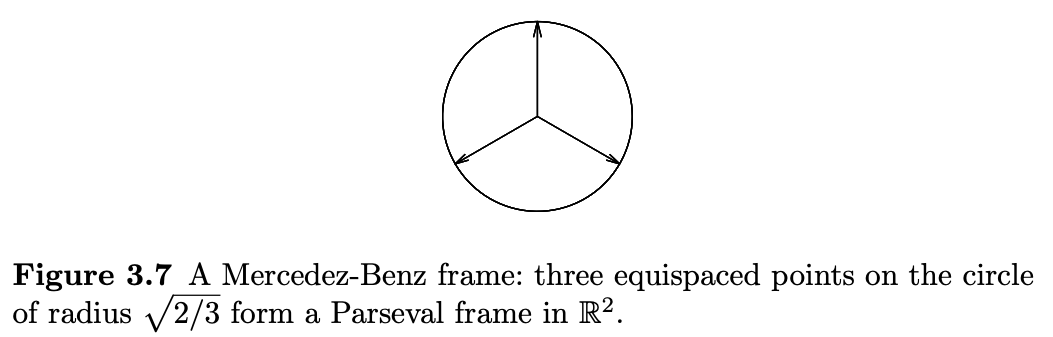
\includegraphics[width=0.8\textwidth]{Chapter 3/fig3-7.png}
\end{center}
\end{example}

Here are two more examples of isotropic distributions:

\begin{example}[Uniform on the discrete cube]
\label{ex:3.3.14}
Let $X$ be a Rademacher random vector, that is, 
\[ X \sim \mnathrm{Unif}(\{-1, 1\}^n). \]
Then $X$ is isotropic.
\end{example}

\begin{example}[Product distributions]
\label{ex:3.3.15}
Any random vector $X = (X_1, \dots, X_n)$ whose coordinates $X_i$ are independent random variables with zero 
mean and unit variance is isotropic. 
\end{example}



% ----------3.4----------
\subsection{Subgaussian Distributions in High Dimensions}
\begin{definition}[]
\label{def:3.4.1}
A random vector $X$ in $\mathbb{R}^n$ is called \underline{subgaussian} if the one-dimensional marginals 
$\left\langle X, v \right\rangle$ are subgaussian random variables for all $v \in \mathbb{R}^n$. 

The \underline{subgaussian norm} of $X$ is defined by taking the maximal subgaussian norm of the marginals 
over all unit vectors: 
\[ \lVert X \rVert_{\psi_2} = \sup_{v \in S^{n - 1}} \lVert \left\langle X, v \right\rangle \rVert_{\psi_2}. \]
\end{definition}

Below are some examples :)

\subsubsection{Gaussian, Rademacher, and More}
\begin{lemma}[Distributions with independent subgaussian coordinates]
\label{lem:3.4.2}
Let $X = (X_1, \dots, X_n)$ be a random vector in $\mathbb{R}^n$ with independent, mean zero, subgassian 
coordinates $X_i$. Then $X$ is a subgaussian random vector, and 
\[ \max_{i \leq n} \lVert X_i \rVert_{\psi_2} \leq \lVert X \rVert_{\psi_2} 
\leq C \max_{i \leq n} \lVert X_i \rVert_{\psi_2}. \]
\end{lemma}

\begin{proof}
The lower bound comes from picking $v$ as a standard basis vector in \cref{def:3.4.1}. 

For the upper bound, fix any $v = (v_1, \dots, v_n) \in S^{n - 1}$. Then 
\begin{align*}
	\lVert \left\langle X, v \right\rangle \rVert_{\psi_2}^2 
	&= \lVert \sum_{i = 1}^{n} v_i X_i \rVert_{\psi_2}^2 \\ 
	&\leq C \sum_{i = 1}^{n} \lVert v_i X_i \rVert_{\psi_2}^2 \quad \text{By \cref{prop:2.7.1}} \\
	&= C \sum_{i = 1}^{n} v_i^2 \lVert X_i \rVert_{\psi_2}^2 \\
	&\leq C \max_{i \leq n} \lVert X_i \rVert_{\psi_2}^2.
\end{align*}
Since $v$ is arbitrary, the proof is complete.
\end{proof}

\begin{example}[Rademacher]
\label{ex:3.4.3}
We can immediately get from the above that a Rademacher normal random vector is subgaussian, and 
\[ c_1 \leq \lVert X \rVert_{\psi_2} \leq c_2 \]
where $c_1, c_2 > 0$ are absolute constants.
\end{example}

\begin{example}[Normal]
\label{ex:3.4.4}
We can also get from the above that if $X \sim N(0, I_n)$, then $X$ is subgaussian. Moreover, 
$Y \sim N(0, \Sigma)$ is also subgaussian (Exercise 3.38).
\end{example}


\subsubsection{Uniform on the Sphere}
The projective CLT (\cref{thm:3.3.9}) tells us that the uniform distribution on $\sqrt{n}S^{n - 1}$ has 
approximately Gaussian 1D marginals. In fact, these marginals ar subgaussian:

\begin{theorem}[Uniform distribution on the sphere is subgaussian]
\label{thm:3.4.5}
Let $X \sim \mathrm{Unif}(S^{n - 1})$. Then for any $v \in S^{n - 1}$ and $t \geq 0$, we have 
\[ P(\left\langle X, v \right\rangle \geq t) \leq 2\exp{\left( -\frac{t^2 n}{2} \right)}. \]
In particular, $X$ is subgaussian, and $\lVert X \rVert_{\psi_2} \leq C / \sqrt{n}$.
\end{theorem}

\begin{proof}
By rotational invariance, we can assume 
\[ X = \frac{g}{\lVert g \rVert_{2}} \text{ where } g \sim N(0, I_n). \]
Again, the distribution of $\left\langle X, v \right\rangle$ does not depend on $v$ hence we can choose 
$v = e_1$ to get $\left\langle X, v \right\rangle = X_1$.

This the inequality $\left\langle X, v \right\rangle \geq t$ becomes $g_1 \geq t \lVert g \rVert_{2}$. 
By squaring both sides, moving $g_1^2$ to the LHS and simplifying, we get 
\[ g_1 \geq s \lVert \bar{g} \rVert_{2}, \quad s = \frac{t}{\sqrt{1 - t^2}} \text{ and } 
\bar{g} = (g_2, \dpts, g_n). \]

To find the probability of the event above, we fix $\lVert \bar{g} \rVert_{2}$ by conditioning on $\bar{g}$, 
which does not alter the distribution of $g$ since $g$ and $\bar{g}$ are independent. Then we uncondition 
by taking the expectation over $\bar{g}$. By the tower property, 
\[ P(\left\langle X, v \right\rangle \geq t) 
= P(g_1 \geq s \lVert \bar{g} \rVert_{2}) = \mathbb{E}[P(g_1 \geq s \lVert \bar{g} \rVert_{2}) \ | \ \bar{g}] 
\quad (*). \]

After conditioning, the conditional probability above reduces to a gaussian tail. By exercise 2.6, 
we get that 
\[ \mathbb{E}[P(g_1 \geq s \lVert \bar{g} \rVert_{2}) | \bar{g}] 
\leq \mathbb{E}[\exp{\left( -\frac{s^2 \lVert g \rVert_{2}^2}{2} \right)}] 
= \left[ \mathbb{E}[\exp{\left( -\frac{s^2 g_1^2}{2} \right)}] \right]^{n - 1}. \]
where the last equality comes from the fact that $g_i$ are i.i.d. $N(0, 1)$ random variables, and 
\[ \lVert \bar{g} \rVert_{2}^2 = g_2^2 + \cdots + g_n^2. \]
For the expression above, 
\begin{align*}
	\mathbb{E}[\exp{(-s^2 g_1^2 / 2)}] 
	&= \int_{-\infty}^{\infty} \exp{(-s^2 x^2 / 2)} \cdot 
	\frac{1}{\sqrt{2 \pi}} e^{-x^2 / 2} \ dx \\
	&= \int_{-\infty}^{\infty} \frac{1}{\sqrt{2 \pi}} \exp{\left( -\frac{(\sqrt{1 + s^2}x)^2}{2} \right)} \ dx \\
	&= \frac{1}{\sqrt{1 + s^2}} \int_{-\infty}^{\infty} e^{-v^2 / 2} \ dv \quad (v = \sqrt{1 + s^2}x) \\
	&= \frac{1}{\sqrt{1 + s^2}}.
\end{align*}
Thus the expression above becomes 
\[ \left( \frac{1}{1 + s^2} \right)^{\frac{n - 1}{2}} = (1 - t^2)^{\frac{n - 1}{2}} 
\leq \exp{\left( -\frac{t^2(n - 1)}{2} \right)} \]
since $1 - x \leq e^{-x}$ for all $x \in \mathbb{R}$. 

For the expression (*), the probability is zero for $t \geq 1$ since $\left\langle X, v \right\rangle \leq 
\lVert X \rVert_{2} \lVert v \rVert_{2} = 1$, while for $t \leq 1$, 
\[ \exp{(-t^2(n - 1) / 2)} \leq e^{1/2}\exp{(-t^2 n / 2)} \leq 2\exp{(-t^2 n / 2)} \]
and we are done.
\end{proof}

\subsubsection{Non-examples}
Some distributions in $\mathbb{R}^n$ are subgaussian, but their subgaussian norm is huge, therefore it is 
impractical to work with them. Below are a few examples.

\begin{example}[Uniform on a convex body]
\label{ex:3.4.6}
Let $K \subset \mathbb{R}^n$ be convex, and $X \sim \mathrm{Unif}(K)$ be isotropic. Qualitatively, $X$ is 
subgaussian since $K$ is bounded. But quantitatively what is it like? Is it bounded by some constant $C$?

This is true for some isotropic convex bodies like the unit cube $[-1, 1]^n$ (\cref{lem:3.4.2}) and 
the Euclidean ball of radius $\sqrt{n + 2}$ (Exercise 3.25 \& 3.42). However, for other convex bodies like the 
ball in the $ell^1$ norm, the subgaussian norm can grow with $n$ (Exercise 3.44).

Even so, a weaker result holds: $X$ has subexponential marginals, and 
\[ \lVert \left\langle X, v \right\rangle \rVert_{\psi_1} \leq C \]
for all unit vectors $v$, which comes from C. Borell's lemma, which follows from the Brunn-Minkowski inequality.
\end{example}

\begin{example}[Coordinate distribution]
\label{ex:3.4.7}
Let $X \sim \mathrm{Unif}\{\sqrt{n}e_1, \dots, \sqrt{n}e_n\}$. $X$ is subgaussian as it takes on finitely 
many values. However, from Exercise 3.43, 
\[ \lVert X \rVert_{\psi_2} \asymp \sqrt{\frac{n}{\log{n}}}. \]
Therefore it is not useful to think of $X$ as subgaussian.
\end{example}

\begin{example}[Discrete distributions]
\label{ex:3.4.8}
Some isotropic discrete distributions have subgaussian norm bounded by a constant, like the Rademacher 
distribution. However, they must take exponentially many values (Exercise 3.46). In particular, this prevents 
frames (\cref{prop:3.3.11}) as good subgaussian distributions as they take way too many values and are mostly 
useless in practice.
\end{example}


% ----------3.5----------
\subsection{Application: Grothendieck Inequality and Semidefinite Programming}
In this section, we will used high-dimensional Gaussians to tackle problems that are seemingly not related 
to probability at all. We first present the Grothendieck inequality.

\begin{theorem}[Grothendieck inequality]
\label{thm:3.5.1}
Consider $a \in \mathbb{R}^{m \times n}$. Assume that 
\[ \left| \sum_{i, j}^{} a_{ij} x_i y_j \right| \leq 1 \text{ for any numbers } x_i, y_j \in \{-1, 1\}. \]
Then for any Hilbert space $H$, we have 
\[ \left| \sum_{i, j}^{} a_{ij} \left\langle u_i, v_j \right\rangle \right| \leq K \text{ for any unit 
vectors } u_i, v_j \in H. \]
Here $K \leq 1.783$ is an absolute constant.
\end{theorem}

There is nothing random in the statement above, but we'll approach it using probabilistic reasoning. In fact, 
there will be two proofs for Grothendieck inequality, one with a much worse bound of $K \leq 14.1$ in this 
section, and the other one with $K \leq 1.783$ in section 3.7. Before going into the first argument, 
there is a simple observation that we state here.

\begin{remark}[Homogeneous form of Grothendieck inequality]
\label{rmk:3.5.2}
The assumption of Grothendieck inequality can be equivalently stated as 
\[ \left| \sum_{i, j}^{} a_{ij}x_iy_j \right| \leq \max_{i}|x_i| \cdot \max_{j}|y_j| \]
for any real numbers $x_i$ and $y_j$ (Exercise 3.47). The conclusion of Grothendieck inequality can be 
equivalently stated as
\[ \left| \sum_{i, j}^{} a_{ij} \left\langle u_i, v_j \right\rangle \right| 
\leq K \max_{i} \lVert u_i \rVert_{} \cdot \max_{j} \lVert v_j \rVert_{} \]
for any Hilbert space $H$ and any vectors $u_i, v_j, \in H$ via rescaling.
\end{remark}

\begin{proof}[Proof of \cref{thm:3.5.1} with worse bound]
(\textbf{Step 1: Reductions}) Note that Grothendieck inequality becomes trivial if we allow the value of $K$ to 
depende on the matrix $A = (a_{ij})$. For example, $K = \sum_{i, j}^{} |a_{ij}|$ would work! Let $A(K)$ be the 
smallest number that makes the conclusion in \cref{rmk:3.5.2} holds for a given matrix $A$ and any Hilbert 
space $H$ and any vectors $u_i, v_j \in H$. Our goal is to show that $K$ is actually \textit{independent} of 
both the matrix $A$ and the dimensions $m$ and $n$.

WLOG, we may show this for a specific Hilbert space $H$, namely for $\mathbb{R}^N$ equipped with the Euclidean 
norm $\lVert \cdot \rVert_{2}$. This is because we can replace $H$ with the subspace spanned by the vectors 
$u_i$ and $v_j$, which has dimension at most $N = m + n$ and inherits the norm from $H$. Then, we use the fact 
that all $N$-dimensional Hilbers spaces are isometric to $\mathbb{R}^N$ with the usual Euclidean norm 
$\lVert \cdot \rVert_{2}$. This isometry can be built by matching a given orthonormal basis of $H$ with the 
canonical bases of $\mathbb{R}^N$.

By the definition of $K = K(A)$, there exist vectors $u_i, v_j \in \mathbb{R}^N$ satisfying 
\[ \sum_{i, j}^{} a_{ij}\left\langle u_i, v_j \right\rangle = K, \ 
\lVert u_i \rVert_{2} = \lVert v_j \rVert_{2} = 1. \]

(\textbf{Step 2: Introducing randomness}) The key idea of the proof is to express the vectors $u_i, v_j$ 
using Gaussian random variables 
\[ U_i := \left\langle g, u_i \right\rangle \text{ and } V_j := \left\langle g, v_j \right\rangle, 
\text{ where } g \sim N(0, I_N). \]
Then $U_i$ and $V_j$ are standard normal random variables whose correlations follow exactly the inner products 
of the vectors $u_i$ and $v_j$ (\cref{cor:3.3.2} and Exercise 3.9):
\[ \mathbb{E}\left[ U_iV_j \right] = \left\langle u_i, v_j \right\rangle. \]
Thus 
\[ K = \sum_{i, j}^{}a_{ij} \left\langle u_i, v_j \right\rangle 
= \mathbb{E}\left[ \sum_{i, j}^{}a_{ij}U_iV_j \right] \quad (*). \]

Suppose for a moment that the random variables $|U_i|$ and $|V_j|$ were to be almost surely bounded by some 
constant, say $R$. Then from the assumption in \cref{rmk:3.5.2}, 
\[ \left| \sum_{i, j}^{} a_{ij}U_iV_j \right| \leq R^2 \text{ almost surely. } \]
Plugging this into the equation above will give $K \leq R^2$, completing the proof.

(\textbf{Step 3: Truncation}) The above is flawed, because the Gaussian random variables $U_i, V_j$ are 
unbounded. But their tails are light enough that they are close to being bounded. To act on this heuristic, we 
use a \textit{truncation} trick. Pick a level $R \geq 1$ and split the random variables like this:
\[ U_i = U_i^- + U_i^+ \text{ where } U_i^- = U_i \mathbf{1}_{\{|U_i| \leq R\}} \text{ and } 
U_i^+ = U_i \mathbf{1}_{\{|U_i| > R\}}. \]
We similarly decompose $V_j = V_j^- + V_j^+$. Nor $U_i^-$ and $V_j^-$ are bounded by $R$, as desired. The 
remainder terms $U_I^+$ and $V_j^+$ are small in the $L^2$ norm: by Exercise 2.4 (b), a Gaussian tail bound 
gives 
\[ \lVert U_i^+ \rVert_{L^2}^2 \leq 2 \left( R + \frac{1}{R} \right) \frac{1}{\sqrt{2 \pi}}e^{-R^2 / 2} 
< \frac{4}{R^2} \quad (**). \]
A similar bound holds for $V_j^+$.

(\textbf{Step 4: Breaking up the sum}) Replacing $U_i V_j$ with $(U_i^- + U_i^+)(V_j^- + V_j^+)$ in $(*)$ and 
expanding the sum, we get 
\[ K = \underbrace{\mathbb{E}\left[ \sum_{i, j}^{} a_{ij} U_i^- V_j^- \right]}_{S_-}
+ \underbrace{\mathbb{E}\left[ \sum_{i, j}^{} a_{ij} U_i^+ V_j^- \right]}_{S_{\pm}}
+ \underbrace{\mathbb{E}\left[ \sum_{i, j}^{} a_{ij} U_i^- V_j^+ \right]}_{S_{\mp}} 
+ \underbrace{\mathbb{E}\left[ \sum_{i, j}^{} a_{ij} U_i^+ V_j^+ \right]}_{S_+}. \]
Let's bound each term! $S_-$ is the easiest to bound: by construction, $|U_i|$ and $|V_j|$ are bounded by $R$, 
so from step 2 we can directly get that 
\[ S_- \leq R^2. \]

We cannot use the same reasoning for $S_{\pm}$, since the random variable $U_i^+$ is unbounded. Instead, let 
us treat the random variables $U_i^+$ and $V_j^-$ as elements of the Hilbert space $L^2$ with the inner product 
$\left\langle X, Y \right\rangle_{L^2} = \mathbb{E}\left[ XY \right]$. Thus write 
\[ S_{\pm} = \sum_{i, j}^{} a_{ij} \left\langle U_i^+, V_j^- \right\rangle_{L^2}. \]
We have $\lVert U_i^+ \rVert_{L^2} < 2/R$ by $(**)$, and $\lVert V_j^- \rVert_{L^2} \leq 
\lVert V_j \rVert_{L^2} = 1$ by construction. Then, applying the conclusion from \cref{rmk:3.5.2} for the 
Hilbert space $H = L^2$, we find that 
\[ S_{\pm} = K \cdot \frac{2}{R}. \]
(It might seem odd that we are using the inequality that we are trying to prove. However, we picked 
$K = K(A)$ at that start to be the smallest value to make Grothendieck inequality work. That is the $K$ that 
we are using here).

The last two terms, $S_{\mp}$ and $S_+$, can be bounded just like the above (Check).

(\textbf{Step 5: Putting everything together}) Plugging the bounde on all four terms, we conclude that 
\[ K \leq R^2 + \frac{6K}{R}. \]
Setting $R = 12$ and rearranging the terms gives $K \leq 288$. A litte finer analysis, skipping the rough 
$4 / R^2$ bound in $(**)$ yields $K \leq 14.1$ (Exercise 3.48).
\end{proof}

\begin{remark}[Quadratic Grothendieck]
\label{rmk:3.5.3}
We can often relax Grothendieck inequality by taking $x_i = y_i$, bounding a quadratic instead of a bilinear 
form. The statement becomes: Let $A \in \mathbb{R}^{n \times n}$ be symmetric PSD or diagonal-free. Assume that 
\[ \left| \sum_{i, j}^{} a_{ij}x_ix_j \right| \leq 1 \text{ for any numbers } x_i \in \{-1, 1\}. \]
Then for any Hilbert space $H$, we have 
\[ \left| \sum_{i, j}^{} a_{ij}\left\langle u_i, v_j \right\rangle \right| \leq 2K \text{ for any unit vectors} 
u_i, v_j \in H. \]
Here $K$ is the the absolute constant from Grothendieck inequality.
\end{remark}

\begin{proof}
Exercises 3.49 \& 3.50.
\end{proof}



% ----------3.6----------
\subsection{Application: Maximum Cut for Graphs}




% ----------3.7----------
\subsection{Kernel Trick and Tightening of Grothendieck Inequaltity}



\section{Random Matrices}

This chapter mostly focuses on the theory regarding random matrices - nets, covering and packing numbers. 
Applications include community detection, covariance estimation, and spectral clustering.



% ----------4.1----------
\subsection{A Quick Refresher on Linear Algebra}

\subsubsection{Singular Value Decomposition}
\begin{theorem}[SVD]
\label{thm:4.1.1}
Any $m \times n$ matrix $A$ with real entries can be written as 
\[ A = \sum_{i = 1}^{r} \sigma_i u_i v_i^T \text{ where } r = \min_{}(m, n). \]
Here $\sigma_i > 0$ are the \underline{singular values} of $A$, $u_I \in \mathbb{R}^m$ are orthonormal vectors 
called the \underline{left singular vectors} of $A$, and $v_i \in \mathbb{R}^n$ are orthonormal vectors called 
the \underline{right singular vectors} of $A$.
\end{theorem}

\begin{proof}
WLOG, we can assume that $m \geq n$ or else we can just take the transpose. Since $A^T A \in \mathbb{R}^
{n \times n}$ is a symmetric positive semidefinite matrix, the spectral theorem tells us that its eigenvalues 
are $\sigma_1^2, \dots, \sigma_n^2$ and corresponding orthonormal eigenvectors $v_1, \dots, v_n \in 
\mathbb{R}^n$, so that $A^T A v_i = \sigma_i^2 v_i$. The vectors $Av_i$ are orthogonal: 
\[ \left\langle Av_i, Av_j \right\rangle = \left\langle A^TA v_i, v_j \right\rangle 
= \sigma_i^2 \left\langle v_i, v_j \right\rangle = \sigma_i^2 \delta{ij}. \]
Therefore, there exist orthonormal vectors $u_1, \dots, u_n \in \mathbb{R}^n$ such that 
\[ Av_i = \sigma_i u_i, \quad i = 1, \dots, n. \]
For the above, for all $i$ with $\sigma_i \neq 0$, the vectors $u_i$ are uniquely defined and ensures that 
they are orthonormal. If $\sigma_i = 0$, then $Av_i = 0$ holds triviall. In this case, we can pick any $u_i$ 
while keeping orthonormality.

Since $v_1, \dots, v_n$ form an orthonormal basis of $\mathbb{R}^n$, we can write $I_n = \sum_{i = 1}^{n} 
v_i v_i^T$. Multiplying by $A$ on the left and plugging the equation above gives 
\[ A = \sum_{i = 1}^{n} (Av_i)v_i^T = \sum_{i = 1}^{n} \sigma_i u_i v_i^T. \]
\end{proof}

\begin{remark}[Geometric interpretation]
\label{rmk:4.1.2}
SVD gives a geometric view of matrices: it stretches the orthogonal direction of $v_i$ by $\sigma_i$, then 
rotates the space, mapping the orthonormal basis $v_i$ to $u_i$.
\end{remark}

\begin{remark}[SVD matrix form]
\label{rmk:4.1.3}
We can set $\sigma_i = 0$ for $i > r$ and arrange them in weakly decreasing order. Then by extending 
$\{u_i\}$ and $\{v_i\}$ to orthonormal bases in $\mathbb{R}^m$ and $\mathbb{R}^n$, we get 
\[ A = U \Sigma V^T \]
where $U$ is the $m \times m$ matrix with left singular vectors $u_i$ as columns, $V$ is the $n \times n$ 
orthogonal matrix with right singular vectors $v_i$ as columns, and $\Sigma$ is the $m \times n$ diagonal 
matrix with the singular values $\sigma_i$ on the diagonal. If $A$ is symmetric, we get the spectral 
decomposition instead: 
\[ A = U \Lambda U^T. \]
\end{remark}

\begin{remark}[Spectral decomposition v.s. SVD]
\label{rmk:4.1.4}
The spectral and singular value decompositions are tightly connected. Since 
\[ AA^T = \sum_{i = 1}^{r} \sigma_i^2 u_i u_i^T \text{ and } A^T A = \sum_{i = 1}^{r} \sigma_i^2 v_i v_i^T \]
the left singular vectors $u_i$ of $A$ are the eigenvectors of $AA^T$, while the right singular vectors $v_i$ 
of $A$ are the eigenvectors of $A^T A$, and the singular values $\sigma_i$ of $A$ are 
\[ \sigma_i(A) = \sqrt{\lambda_i(AA^T)} = \sqrt{\lambda_i(A^T A)}. \]
\end{remark}

\begin{remark}[Orthogonal projection]
\label{rmk:4.1.5}
Consider the orthogonal projection $P$ in $\mathbb{R}^n$ onto a $k$-dimensional subspace $E$. The projection 
of a vector $x$ onto $E$ is given by $Px = \sum_{i = 1}^{k} \left\langle u_i, x \right\rangle u_i$ where 
$u_1, \dots, u_k$ is an orthonormal basis of $E$. We can rewrite this as 
\[ P = \sum_{i = 1}^{k} u_i u_i^T = UU^T \]
where $U$ is the $n \times k$ matrix with orthonormal columns $u_i$. In particular, $P$ is a symmetric 
matrix with eigenvalues $\underbrace{1, \dots, 1}_{k}, \underbrace{0, \dots, 0}_{n - k}$.
\end{remark}

\subsubsection{Min-max Theorem}
\label{thm:4.1.6}
There is another optimization-based description of eigenvalues:
\begin{theorem}[Min-max theorem for eigenvalues]
The $k$-th largest eigenvalue of an $n \times n$ symmetric matrix $A$ can be written as 
\[ \lambda_k(A)= \max_{\dim{E} = k} \min_{x \in S(E)} x^T Ax 
= \min_{\dim{E} = n-k+1} \max_{x \in S(E)} x^T Ax, \]
where the first max/min is taking with respect to all subspaces of a fixed dimension, and $S(E)$ denotes 
the Euclidean unit sphere of $E$, i.e. the set of all unit vectors in $E$. 
\end{theorem}

\begin{proof}
Let us focus on the first equation. To prove the upper bound on $\lambda_k$, we need to find a $k$-dimensional 
subspace $E$ such that 
\[ x^T Ax \geq \lambda_k \text{ for all } x \in S(E). \]
To find the set $E$, take the spectral decomposition $A = \sum_{i = 1}^{n} \lambda_i u_i u_i^T$ and pick the 
subspace $E = \mathrm{span}(u_1, \dots, u_k)$. The eigenvectors form an orthonormal basis of $E$, so any vector 
$x \in S(E)$ can be written as $x = \sum_{i = 1}^{k} a_i u_i$. Then by orthonormality of $u_i$ and 
monotonicity of $\lambda_i$, we get 
\[ x^T Ax = \sum_{i = 1}^{k} \lambda_i a_i^2 \leq \lambda_k \sum_{i = 1}^{k} a_i^2 = \lambda_k \]
and we have the upper bound. For the lower bound on $\lambda_k$, we need to find $x \in S(E)$ such that 
$x^T Ax \leq \lambda_k$. Here we let the subspace be $F = \mathrm{span}(u_k, \dots, u_n)$. 

Since $\dim{E} + \dim{F} = n + 1$, the intersection of $E$ and $F$ is nontrivial hence there is a unit 
vector $x \in E \cap F$.  Writing $x = \sum_{i = k}^{n} a_i u_i$, we get 
\[ x^T Ax = \sum_{i = k}^{n} \lambda_i a_i^2 \geq \lambda_k \sum_{i = k}^{n} a_i^2 = \lambda_k. \]
Then we get the lower bound, and hence the first equality is done.

The second equality is by applying the same technique to $-A$ and reversing the eigenvalues.
\end{proof}

Applying \cref{thm:4.1.6} to $A^T A$ and using \cref{rmk:4.1.4}, we get 
\begin{corollary}[Min-max theorem for singular values]
\label{cor:4.1.7}
Let $A \in \mathbb{R}^{m \times n}$ with singular values $\sigma_1 \geq \cdots \geq \sigma_n \geq 0$. Then 
\[ \sigma_k(A) = \max_{\dim{E} = k} \min_{x \in S(E)} \lVert Ax \rVert_{2} 
= \min_{\dim{E} = n-k+1} \max_{x \in S(E)} \lVert Ax \rVert_{2} \]
with the same notation as \cref{thm:4.1.6}.
\end{corollary}

\subsubsection{Frobenius and Operator Norms}
\begin{definition}[]
\label{def:4.1.8}
For a matrix $A \in \mathbb{R}^{m \times n}$, the \underline{Frobenius norm} is 
\[ \lVert A \rVert_{F} := \left( \sum_{i = 1}^{m} \sum_{j = 1}^{n} A_{ij}^2 \right)^{1/2}. \]

The \underline{operator norm} of $A$ is the smallest number $K$ such that 
\[ \lVert Ax \rVert_{2} \leq K \lVert x \rVert_{2} \text{ for all } x \in \mathbb{R}^n. \]
Equivalently, 
\[ \lVert A \rVert_{} = \max_{x \neq 0} \frac{\lVert Ax \rVert_{2}}{\lVert x \rVert_{2}} 
= \max_{\lVert x \rVert_{2} \leq 1} \lVert Ax \rVert_{2} 
= \max_{\lVert x \rVert_{2} = 1} \lVert Ax \rVert_{2} 
= \max_{\lVert x \rVert_{2} = \lVert y \rVert_{2} = 1} |y^T Ax|. \]
\end{definition}
From the Frobenius norm, we can get that 
\[ \left\langle A, B \right\rangle = \sum_{i = 1}^{m} \sum_{j = 1}^{n} A_{ij} B_{ij} = \mathrm{tr}(A^T B). \]
Also, from above we can get 
\[ \lVert A \rVert_{F}^2 = \left\langle A, A \right\rangle = \mathrm{tr}(A^T A). \]

For the operator norm, the first three equations follows by rescaling, and the last one comes from the 
duality formula: 
\[ \lVert Ax \rVert_{} = \max_{\lVert y \rVert_{2} = 1} \left\langle Ax, y \right\rangle. \]
Here the absolute sign does not matter.

\begin{remark}[Other operator norms]
\label{rmk:4.1.9}
We can replace the $\ell^2$ norm in \cref{def:4.1.8} with other norms to get a more general concept of 
operator norms (Exercise 4.18-4.22).
\end{remark}

\subsubsection{The Matrix Norms and the Spectrum}
\begin{lemma}[Orthogonal invariance]
\label{lem:4.1.10}
The Frobenius and spectral norms are orthogonal invariant, meaning that for any $A$ and orthogonal matrices 
$Q, R$ with proper dimensions, we have 
\[ \lVert QAR \rVert_{F} = \lVert A \rVert_{F} \text{ and } \lVert QAR \rVert_{} = \lVert A \rVert_{}. \]
\end{lemma}

\begin{proof}
For the Frobenius norm, by one of the formulas above, 
\begin{align*}
	\lVert QAR \rVert_{F} 
	&= \mathrm{tr}(R^T AT Q^T QAR) \\
	&= \mathrm{tr}(R^T A^T AR) \\
	&= \mathrm{tr}(RR^T A^T A) \\
	&= \mathrm{tr}(A^T A) \\
	&= \lVert A \rVert_{F}^2.
\end{align*}
For the spectral norm, by an equivalent characterization, $\lVert QAR \rVert_{}$ is obtained by maximizing the 
bilinear form $y^T QARx = (Qy)^T A (Rx)$ over all unit vectors $x, y$. Since $Q, R$ are orthogonal, 
$Qy$ and $Rx$ also range over all unit vectors, so we just get $\lVert A \rVert_{}$ as a result.
\end{proof}

\begin{lemma}[Matrix norms via singular values]
\label{lem:4.1.11}
For any $A \in \mathbb{R}^{m \times n}$ with singular values $\sigma_1 \geq \cdots \geq \sigma_n$, 
\[ \lVert A \rVert_{F} = \left( \sum_{i = 1}^{n} \sigma_i^2 \right)^{1/2} \text{ and } 
\lVert A \rVert_{} = \sigma_1. \]
\end{lemma}

\begin{proof}
For the Frobenius norm, by orthogonal invariance (\cref{lem:4.1.10}), 
\[ \lVert A \rVert_{F} = \lVert U \Sigma V^T \rVert_{F} = \lVert \Sigma \rVert_{F} \]
which directly gives us the result.

The result for the operator norm directly follows from \cref{cor:4.1.7} with $k = 1$.
\end{proof}

\begin{remark}[Symmetric matrices]
\label{rmk:4.1.12}
For a symmetric matrix $A$ with eigenvalues $\lambda_k$, 
\[ \lVert A \rVert_{} = \max_{k}|\lambda_k| = \max_{\lVert x \rVert_{} = 1} |x^T Ax|. \] 
The first equality becomes \cref{lem:4.1.11} since the singular values of $A$ are $|\lambda_k|$. The 
min-max theorem (\cref{thm:4.1.6}) gives $|\lambda_k| \leq \max_{\lVert x \rVert_{} = 1} |x^T Ax|$, proving 
the upper bound in the equation above. The lower bound can be proven by taking $x - y$ in the definition of 
the operator norm (\cref{def:4.1.8}).
\end{remark}

\subsubsection{Low-rank Approximation}
For a given matrix $A$, what is the closest approximation to it for a given matrix of rank $k$? The answer 
is just truncating the SVD of A: 

\begin{theorem}[Eckart-Young-Mirski theorem]
\label{thm:4.1.13}
Let $A = \sum_{i = 1}^{n} \sigma_i u_i v_i^T$. Then for any $1 \leq k \leq n$,
\[ \min_{\mathrm{rank}(B) = k} \lVert A - B \rVert_{} = \sigma_{k + 1}. \]
The minimum is attained at $B = \sum_{i = 1}^{k} \sigma_i u_i v_i^T$.
\end{theorem}

\begin{proof}
If $B \in \mathbb{R}^{m \times n}$ has rank $k$, $\dim{\ker{(B)}} = n - k$. Then the min-max theorem 
(\cref{cor:4.1.7}) for $k + 1$ instead of $k$ gives 
\[ \lVert A - b \rVert_{} \geq \max_{x \in S(E)} \lVert (A - B)x \rVert_{2} 
= \max_{x \in S(E)} \lVert Ax \rVert_{2} \geq \sigma_{k + 1}. \]

In the opposite direction, setting $B = \sum_{i = 1}^{k} \sigma_i u_i v_i^T$ gives $A - b = 
\sum_{i = k + 1}^{n} \sigma_i u_I v_i^T$. The maximal singular value of this matrix $\sigma_{k + 1}$, 
which is the same as its operator norm by \cref{lem:4.1.11}.
\end{proof}

\subsubsection{Perturbation Theory}
We can also study how eigenvalues/eigenvectors change under matrix perturbations: 
\begin{lemma}[Weyl inequality]
\label{lem:4.1.14}
The $k$-th largest eigenvalue of symmetric matrices $A, B$ satisfy 
\[ |\lambda_k(A) - \lambda_k(B)| \leq \lVert A - B \rVert_{}. \]
Similarly, the $k$-th largest singular values of general rectangular matrices satisfy 
\[ |\sigma_k(A) - \sigma_k(B)| \leq \lVert A - B \rVert_{}. \]
\end{lemma}

A similar result holds for eigenvectors, however we have to track the same eigenvector before and after the 
perturbation. If the eigenvalues are too close, a small perturbation can swap them, leading to huge error 
since their eigenvectors are orthogonal and far apart.

\begin{theorem}[Davis-Kahan inequality]
\label{thm:4.1.15}
Consider two symmetric matrices $A, B$ with spectral decompositions 
\[ A = \sum_{i = 1}^{n} \lambda_i u_i u_i^T, \ B = \sum_{i = 1}^{n} \mu_i v_i v_i^T, \]
where the eigenvalues are weakly decreasing. Assume the the $k$-th largest eigenvalue of $A$ is 
$\delta$-seperated from the rest: 
\[ \min_{i \neq k} |\lambda_k - \lambda_i| = \delta > 0. \]
Then the angle between the eigenvectors $u_k$ and $v_k$ satisfies
\[ \sin{\angle u_k, v_k} \leq \frac{2 \lVert A - B \rVert_{}}{\delta}. \]
\end{theorem}

The theorem above can be derived via a stronger result of Davis-Kahan focusing on spectral projections - 
the orthogonal projections onto the span of some subset of eigenvectors:

\begin{lemma}[Davis-Kahan inequality for spectral projections]
\label{lem:4.1.16}
Consider $A, B$ as in \cref{thm:4.1.15}. Let $I, J$ be two $\delta$-seperated subsets of $\mathbb{R}$, with 
$I$ being an interval. Then the spectral projections 
\[ P = \sum_{i: \lambda_i \in I}^{} u_i u_i^T \text{ and } 
Q = \sum_{j: \lambda_j \in J}^{} v_j v_j^T \text{ satisfy } \lVert QP \rVert_{} 
\leq \frac{\lVert A - B \rVert_{}}{\delta}. \]
\end{lemma}

\begin{proof}
WLOG, assume $I$ is finite and closed. Adding the same multiple of Identity to $A$ and $B$, we can center 
$I$ as $[-r, r]$, so that $|\lambda_i| \leq r$ for $i \in I$ and $|\mu_j| \geq r + \delta$ for $\mu_j \in J$. 
The idea is to see how $P$ and $Q$ interact through $H := B - A$:
\[ \lVert H \rVert_{} \geq \lVert QHP \rVert_{} = \lVert QBP - QAP \rVert_{} 
\geq \lVert QBP \rVert_{} - \lVert QAP \rVert_{}. \]
The spectral projection $A$ commutes with $B$, hence 
\[ \lVert QBP \rVert_{} \geq \lVert BQP \rVert_{} \geq (r + \delta)\lVert QP \rVert_{}. \]
To see the last inequality, the image of $Q$ is spanned by orthogonal vectors $v_j$ with $|\mu_j| \geq 
r + \delta$. The matrix $B$ maps each such vector $v_j$ to $\mu_j v_j$, hence scaling it by at least 
$r + \delta$. Thus $B$ expands the norm of any vector in the image of $Q$ by at least $r + \delta$ so
\[  \lVert BQPx \rVert_{2} \geq (r + \delta)\lVert QPx \rVert_{2} \text{ for any } x. \]
Taking the supremum over all unit vectors gives the result with the operator norm. 

Also, $AP = PAP = \sum_{i: \lambda_i \in I}^{} \lambda_i u_i u_i^T$ so 
\[ \lVert QAP \rVert_{} = \lVert QPAP \rVert_{} \leq \lVert QP \rVert_{} \cdot \lVert AP \rVert_{} 
\leq r \lVert AP \rVert_{}, \]
because $\lVert AP \rVert_{} = \max_{i: \lambda_i \in I} |\lambda_i| \leq r$. Putting the two bounds together 
we get 
\[ \lVert H \rVert_{} = \lVert B - A \rVert_{} \geq \delta \lVert QP \rVert_{}, \]
which completes the proof.
\end{proof}

\begin{proof}[Proof for \cref{thm:4.1.15}]
Since the LHS is a trig angle, we can assume that $\varepsilon := \lVert A - B \rVert_{} \leq \delta / 2$ or 
else the inequality holds trivially. By Weyl inequality (\cref{lem:4.1.14}), $|\lambda_j - \mu_j| 
\leq \varepsilon$ for each $j$ hence 
\[ \min_{j: j \neq k} |\lambda_k - \mu_k| \geq \min_{j: j \neq k} |\lambda_k - \lambda_j| - \varepsilon 
= \delta - \varepsilon \geq \delta/2. \]
Apply \cref{lem:4.1.16} for the $\delta/2$-seperated subsets $I = \{\lambda_k\}$ and $J = \{\mu_j: 
j \neq k\}$ to get $\lVert QP \rVert_{} \leq 2 \varepsilon / \delta$. 

Since $P$ and $I_n - Q$ are the orthogonal projections on the directions of $u_k$ and $v_k$ respectively, 
\[ \lVert QP \rVert_{} = \max_{\lVert x \rVert_{} = 1} \lVert QPx \rVert_{2} 
= \lVert Q u_k \rVert_{2} = \sin{\angle(u_k, v_k)}. \]
Combining this with the inequality on $\lVert QP \rVert_{}$ above completes the proof.
\end{proof}

\subsubsection{Isometries}
The singular values of a matrix $A$ satisfy (by the min-max theorem)
\[ \sigma_n \lVert x - y \rVert_{2} \leq \lVert Ax - Ay \rVert_{2} \leq \sigma_1 \lVert x - y \rVert_{2}. \]
The extreme singular values set the limits on how the linear map $A$ distorts space.

A matris is an \underline{isometry} if 
\[ \lVert Ax \rVert_{2} = \lVert x \rVert_{2} \text{ for all } x \in \mathbb{R}^n. \]
Notice that $A$ need not be a square matrix. T

For $A \in \mathbb{R}^{m \times n}$ with $m \geq n$, the following are equivalent: 
\begin{enumerate}
	\item The columns of $A$ are orthonormal, i.e. $A^T A = I_n$, 
	\item A is an isometry, 
	\item All singular values of $A$ are 1.
\end{enumerate}

There is a stronger result where the properties hold approximately instead of exactly (useful when 
dealing with random matrices): 
\begin{lemma}[Approximate isometries]
\label{lem:4.1.17}
Let $A \in \mathbb{R}^{m \times n}$ with $m \geq n$ and let $\varepsilon \geq 0$. The following are equivalent: 
\begin{enumerate}
	\item $\lVert A^T A - I_n \rVert_{} \leq \varepsilon$.
	\item $(1 - \varepsilon)\lVert x \rVert_{2}^2 \leq \lVert Ax \rVert_{2}^2 \leq 
	(1 + \varepsilon)\lVert x \rVert_{2}^2$ for any $x \in \mathbb{R}^n$.
	\item $1 - \varepsilon \leq \sigma_n^2 \leq \sigma_1^2 \leq 1 + \varepsilon$.
\end{enumerate}
\end{lemma}

\begin{proof}
(a) $\Leftrightarrow$ (b) By rescaling, we can assume that $\lVert x \rVert_{2} = 1$ in (b). Then we have 
\[ \lVert A^T A - I_n \rVert_{} = \max_{\lVert x \rVert_{2} = 1} 
|x^T (A^T A - I_n)x| = \max_{\lVert x \rVert_{2} = 1} |\lVert Ax \rVert_{2}^2 - 1|, \]
The above being bounded by $\varepsilon$ is equivalent to (b) for all unit vectors $x$.

(b) $\Leftrightarrow$ (c) follows from the relationship for singular values distorting space from above.
\end{proof}

\begin{remark}[]
\label{rmk:4.1.18}
Here is a more handy version of (a) $\Rightarrow$ (c) in \cref{lem:4.1.17}. For $z \in \mathbb{R}$ and 
$\delta \geq 0$, 
\[ |z^2 - 1| \leq \max_{}(\delta, \delta^2) \implies |z - 1| \leq \delta. \]
Then substituting $\varepsilon = \max_{}(\delta, \delta^2)$, we get 
\[ \lVert A^T A - I_n \rVert_{} \leq \max_{}(\delta, \delta^2)  
\implies 1 - \delta \leq \sigma_n \leq \sigma_1 \leq 1 + \delta. \]
\end{remark}



% ----------4.2----------
\subsection{Nets, Covering, and Packing}
The $\varepsilon$-net argument is useful for analysis of random matrices. It is also connected to ideas like 
covering, packing, entropy, volume, and coding.

\begin{definition}[]
\label{def:4.2.1}
Let $(T, d)$ be a metric space. Consider $K \subset T$ and $\varepsilon > 0$. A subset $\mathcal{N} \subset 
T$ is called an \underline{$\varepsilon$-net} of $K$ is every point in $K$ is within distance $\varepsilon$ 
of some point in $\mathcal{N}$, i.e.
\[ \forall x \in K \exists x_0 \in \mathcal{N}: \ d(x, x_0) \leq \varepsilon. \]
Equivalently, $\mathcal{N}$ is an $\varepsilon$-net of $K$ if the balls of radius $\varepsilon$ centered at 
points in $\mathcal{N}$ cover $K$, like in the figure below:

\begin{center}
	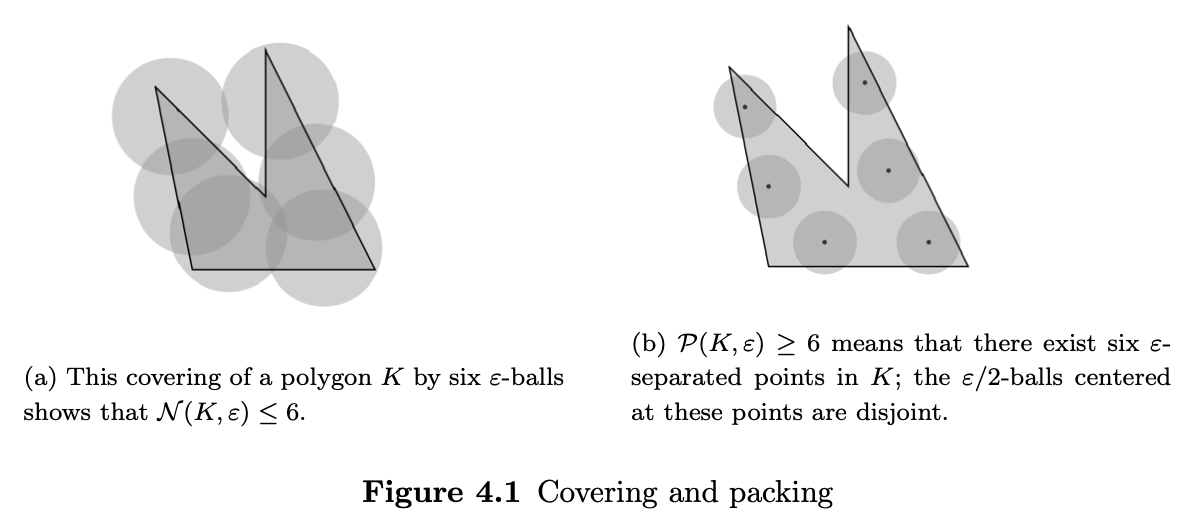
\includegraphics[width=0.8\textwidth]{Chapter 4/fig4-1.png}
\end{center}
\end{definition}

\begin{definition}[]
\label{def:4.2.2}
The smallest cardinality of an $\varepsilon$-net of $K$ is called the \underline{covering number} of 
$K$, and is denoted $\mathcal{N}(K, d, \varepsilon)$.
\end{definition}

\begin{remark}[Compactness]
\label{rmk:4.2.3}
An important result in real analysis says that a subset $K$ of a complete metric space $(T, d)$ is 
\underline{precompact} (i.e. the closure of $K$ is compact) if and only if
\[ N(K, d, \varepsilon) < \infty \text{ for every } \varepsilon > 0. \]
We can think about the covering numbers as a quantitative measure of how compact $K$ is.
\end{remark}

\begin{definition}[]
\label{def:4.2.4}
A subset $\mathcal{N}$ of a metric space $(T, d)$ is \underline{$\varepsilon$-seperated} if 
\[ d(x, y) > \varepsilon \text{ for any distinct points } x, y \in \mathcal{N}. \]
The largest possible cardinality of an $\varepsilon$-seperated subset of a given $K \subset T$ is called 
the \underline{packing number} of $K$ and is denoted $\mathcal{P}(K, d, \varepsilon)$.
\end{definition}

\begin{remark}[Packing balls into $K$]
\label{rmk:4.2.5}
If $\mathcal{N}$ is $\varepsilon$-seperated, the closed $\varepsilon / 2$-balls centered at points in 
$\mathcal{N}$ are disjoint by the triangle inequality, hence we can always pack into $K$ at least 
$\mathcal{P}(K, d, \varepsilon)$ disjoint $\varepsilon / 2$-balls.
\end{remark}

\begin{lemma}[Nets from seperated sets]
\label{lem:4.2.6}
Let $\mathcal{N}$ be a maximal $\varepsilon$-seperated subset of $K$, i.e. adding any new point to $\mathcal{N}$ 
destroys the seperation property. Then $\mathcal{N}$ is an $\varepsilon$-net of $K$.
\end{lemma}

\begin{proof}
Let $x \in K$. We want to show that there exists $x_0 \in \mathcal{N}$ such that $d(x, x_0) \leq \varepsilon$. 
If $x \in \mathcal{N}$, the conclusion is trivial by choosing $x_0 = x$. Suppose $x \notin \mathcal{N}$. 
The maximality assumption implies that $\mathcal{N} \cup \{x\}$ is not $\varepsilon$-seperated, meaning 
$d(x, x_0) \leq \varepsilon$ for some $\varepsilon \in \mathcal{N}$.
\end{proof}

\begin{remark}[Constructing a net]
\label{rmk:4.2.7}
The lemma above (\cref{lem:4.2.6}) gives an iterative algorithm to construct an $\varepsilon$-net for a 
given set $K$. Pick $x_1 \in K$ arbitrarily, then pick $x_2 \in K$ that is farther than $\varepsilon$ from 
$x_1$, then pick $x_3$ that it is farther than $\varepsilon$ from both $x_1$ and $x_2$, and so on. If $K$ 
is compact, then the process will stop in a finite number of iterations!
\end{remark}

\begin{lemma}[Equivalence of covering and packing numbers]
\label{lem:4.2.8}
For any set $K \subset T$ and $\varepsilon > 0$, 
\[ \mathcal{P}(K, d, 2 \varepsilon) \leq \mathcal{N}(K, d, \varepsilon) 
\leq \mathcal{P}(K, d, \varepsilon). \]
\end{lemma}

\begin{proof}
The upper bound follows from \cref{lem:4.2.6} because the packing number is exactly the number that makes 
$\mathcal{N}$ a maximal $\varepsilon$-seperated set.

For the lower bound, take any $2 \varepsilon$-seperated subset $\mathcal{P} = \{x_i\}$ in $K$ and any 
$\varepsilon$-net $\mathcal{N} = \{y_j\}$ of $K$. By definition, each point $x_i$ is in the $\varepsilon$-ball 
centered at some point $y_j$. Since any closed $\varepsilon$ ball cannot contain two $2 \varepsilon$-seperated 
points, each $\varepsilon$-ball centered at $y_j$ can contain at most one $x_i$. The pigeonhole principle 
gives $|\mathcal{P}| \leq |\mathcal{N}|$. Since $\mathcal{P}$ and $\mathcal{N}$ are arbitrary, the bound follows.
\end{proof}

\subsubsection{Covering Numbers and Volume}
This sections is about covers with $T = \mathbb{R}^n$ with the Eudlidean metric 
\[ d(x, y) = \lVert x - y \rVert_{2}. \]
Therefore, we can omit the metric when denoting the covering and packing numbers: 
\[ \mathcal{N}(K, \varepsilon) = \mathcal{N}(K, d, \varepsilon). \]
How do the covering numbers relate to the most classical measure, the volume of $K$ in $\mathbb{R}^n$? 

\begin{definition}[Minkowski sum]
\label{def:4.2.9}
Let $A, B \subseteq \mathbb{R}^n$. The \underline{Minkowski sum} is defined as 
\[ A + B := \{ A + B: \ a \in A, b \in B \}. \]
Below is an example of the Minkowski sum of two sets on the plane:

\begin{center}
	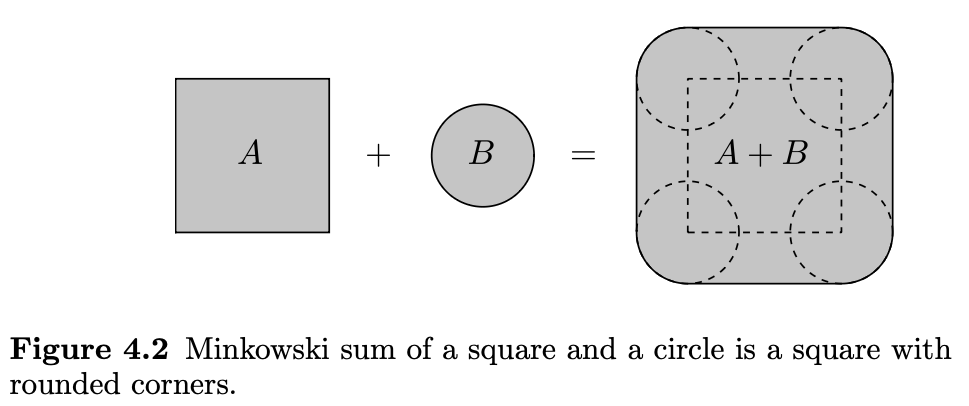
\includegraphics[width=0.8\textwidth]{Chapter 4/fig4-2.png}
\end{center}
\end{definition}

\begin{proposition}[Covering numbers and Volume]
\label{prop:4.2.10}
Let $K \subset \mathbb{R}^n$ and $\varepsilon > 0$. Then
\[ \frac{\mathrm{Vol}(K)}{\mathrm{Vol}(\varepsilon B_2^n)} \leq \mathcal{N}(K, \varepsilon) 
\leq \mathcal{P}(K, \varepsilon) \leq 
\frac{\mathrm{Vol}(K + (\varepsilon / 2)B_2^n)}{\mathrm{Vol}((\varepsilon / 2)B_2^n)}, \]
where $B_2^n$ denotes the unit ball in $\mathbb{R}^n$. 
\end{proposition}

\begin{proof}
The middle inequality was already proven in \cref{lem:4.2.8}, hence we focus on the left and right bounds.

(\textbf{Lower bound}) Let $N := \mathcal{N}(K, \varepsilon)$. Then $K$ can be covered by $N$ balls with radii 
$\varepsilon$. Comparing the volumes,
\[ \mathrm{Vol}(K) \leq N \cdot \mathrm{Vol}(\varepsilon B_2^n), \]
which gives the lower bound.

(\textbf{Upper bound}) Let $N := \mathcal{P}(K, \varepsilon)$. Then we can find $N$ disjoint closed 
$\varepsilon / 2$-balls with centers $x_i \in K$. While these balls may not fit entirely in $K$ (Figure 4-1), 
they do fit in a slightly inflated set, namely $K + (\varepsilon / 2)B_2^n$ (Basically putting balls at the 
boundary of $K$). Comparing the volume gives 
\[ N \cdot \mathrm{Vol}((\varepsilon / 2)B_2^n) \leq \mathrm{Vol}(K + (\varepsilon / 2)B_2^n), \]
which completes the upper bound.
\end{proof}

An important consequence of the volumetric bound is that the covering (hence packing) numbers are typically 
\textit{exponential} in the dimension $n$: 
\begin{corollary}[Covering numbers of the Euclidean ball]
\label{cor:4.2.11}
The covering numbers of the unit Euclidean ball $B_2^n$ satisfy the following for any $\varepsilon > 0$: 
\[ \left( \frac{1}{\varepsilon} \right)^n \leq \mathcal{N}(B_2^n, \varepsilon) 
\leq \left( \frac{2}{\varepsilon} + 1 \right)^n. \]
\end{corollary}

\begin{proof}
The lower bound immediately follows from \cref{prop:4.2.10}, since the volumd in $\mathbb{R}^n$ scale as 
$\mathrm{Vol}(\varepsilon B_2^n) = \varepsilon^n \mathrm{Vol}(B_2^n)$.

The upper bound follows from \cref{prop:4.2.10} as well:
\[ \mathcal{N}(B_2^n, \varepsilon) \leq 
\frac{\mathrm{Vol}((1 + \varepsilon / 2)B_2^n)}{\mathrm{Vol}((\varepsilon / 2)B_2^n)} 
= \frac{(1 + \varepsilon / 2)^n}{(\varepsilon / 2)^n} 
= \left( \frac{2}{\varepsilon} + 1 \right)^n. \]
\end{proof}

To simplify \cref{cor:4.2.11}, we can divide this into two cases for $\varepsilon$:

For $\varepsilon \in (0, 1]$, we have 
\[ \left( \frac{1}{\varepsilon} \right)^n \leq \mathcal{N}(B_2^n, \varepsilon) 
\leq \left( \frac{3}{\varepsilon} \right)^n. \]
In the other case where $\varepsilon > 1$, one $\varepsilon$-ball covers the unit ball hence 
$\mathcal{N}(B_2^n, \varepsilon) = 1$.

\begin{remark}[Volume of the ball]
\label{rmk:4.2.12}
The proof of \cref{cor:4.2.11} works with the volume of the Euclidean ball but never actually calculates it!
We can compute the volume geometrically, probabilistically, and analytically (Exercises 4.27-4.29), and 
also extend this notion of volume to $\ell^p$ balls (Exercise 4.30).
\end{remark}

\begin{remark}[How to construct a net?]
\label{rmk:4.2.13}
We have an algorithm to construct nets already (\cref{rmk:4.2.7}), but for the Euclidean ball, we can also 
use a scaled integer lattice (Exercise 4.31), or just use random points (Exercise 4.39).
\end{remark}

We can also use covering/packing notions for other objects via volumetric arguments, here is another example:

\begin{definition}[]
\label{def:4.2.14} 
The Hamming cube $\{0, 1\}^n$ consists of all binary strings of length $n$. To turn it into a metric space, 
we define the \underline{hamming distance} as the number of bits where the strings $x$ and $y$ differ:
\[ d_H(x, y) := |\{i: \ x(i) \neq y(i) \}|, \ x, y \in \{0, 1\}^n. \]
\end{definition}

\begin{proposition}[Covering and packing numbers of the Hamming cube]
The covering and packing numbers of the Hamming cube $K = \{0, 1\}^n$ satisfy the following for any integer 
$m \in \{0, \dots, n\}$: 
\[ \frac{2^n}{\sum_{k = 0}^{m} \binom{n}{k}} \leq \mathcal{N}(K, d_H, m) 
\leq \mathcal{P}(K, d_H, m) \leq \frac{2^n}{\sum_{k = 0}^{\left\lfloor m/2 \right\rfloor} \binom{n}{k}}. \]
\end{proposition}

\begin{proof}
Use the volumetric argument from above using cardinality instead of the volume (Exercise 4.32).
\end{proof}



% ----------4.3----------
\subsection{Application: Error Correcting Codes}



% ----------4.4----------
\subsection{Upper Bounds on Subgaussian Random Matrices}
This section is mostly concerned with non-asymptotic theory of random matrices. Most of the questions here 
will be about the distributions of singular values, eigenvalues, and eigenvectors.

But before that, we need to know how $\varepsilon$-nets can help compute the operator norm of a matrix.

\subsubsection{Computing the Norm on an \texorpdfstring{$\varepsilon$} -net}
To evaluate $\lVert A \rVert_{}$, we need to control $\lVert Ax \rVert_{2}$ uniformly over the sphere 
$S^{n - 1}$. However, we'll show that instead of the entire sphere, it is enough to control just an 
$\varepsilon$-net of the sphere (in Euclidean metric).

\begin{lemma}[Operator norm on a net]
\label{lem:4.4.1}
Let $A \in \mathbb{R}^{m \times n}$ and $\varepsilon \in (0, 1]$. Then for any $\varepsilon$-net $\mathcal{N}$ 
of the sphere $S^{n - 1}$m we have 
\[ \sup_{x \in \mathcal{N}} \lVert Ax \rVert_{2} \leq \lVert A \rVert_{} 
\leq \frac{1}{1 - \varepsilon} \sup_{x \in \mathcal{N}} \lVert Ax \rVert_{2}. \]
\end{lemma}

\begin{proof}
The lower bound is true since $\mathcal{N} \subset S^{n - 1}$. 

To prove the upper bound, fix a vector $x \in S^{n - 1}$ for which $\lVert A \rVert_{} = \lVert Ax \rVert_{2}$ 
and choose $x_0 \in \mathcal{N}$ such that $\lVert x - x_0 \rVert_{2} \leq \varepsilon$. By the definition 
of the operator norm, this implies 
\[ \lVert Ax - Ax_0 \rVert_{2} \leq \lVert A(x - x_0) \rVert_{2} 
\leq \lVert A \rVert_{} \lVert x - x_0 \rVert_{2} \leq \varepsilon \lVert A \rVert_{}. \]
By the triangle inequality, 
\[ \lVert Ax_0 \rVert_{2} \geq \lVert Ax \rVert_{2} - \lVert Ax - Ax_0 \rVert_{2} 
\geq \lVert A \rVert_{} 0 \varepsilon \lVert A \rVert_{} = (1 - \varepsilon)\lVert A \rVert_{}. \]
Dividing by $1 - \varepsilon$ gives the result.
\end{proof}

There is alsoa version for quadratic forms from the way the operator norm is characterized. Since 
\[ \lVert A \rVert_{} = \max_{x \in S^{n - 1}, y \in S^{m - 1}} 
|\left\langle Ax, y \right\rangle|, \]
we can take $x = y$ and use the spheres' corresponding nets:

\begin{lemma}[Maximizing quadratic forms on a net]
\label{lem:4.4.2}
Let $A \in \mathbb{R}^{m \times n}$ and $\varepsilon \in [0, 1)$. Then for any $\varepsilon$-net $\mathcal{N}$ 
of the sphere $S^{n - 1}$ and any $\varepsilon$ $\varepsilon$-net $\mathcal{M}$ of the sphere $S^{m - 1}$, 
\[ \sup_{x \in \mathcal{N}, y \in \mathcal{M}} |\left\langle Ax, y \right\rangle| 
\leq \lVert A \rVert_{} \leq \frac{1}{1 - 2 \varepsilon} \sup_{x \in \mathcal{N}, y \in \mathcal{M}} 
|\left\langle Ax, y \right\rangle|. \]
Moreover, if $m = n$, $A$ is symmetric, and $\mathcal{N} = \mathcal{M}$, we can take $x = y$.
\end{lemma}

\begin{proof}
There are two methods - one by modifying the proof of \cref{lem:4.4.1} (Exercise 4.36), and a different method 
using $\varepsilon$-net expansions (Exercise 4.34).
\end{proof}

\subsubsection{The Norms of Subgaussian Random Matrices}
\begin{theorem}[Name]
\label{thm:4.4.3}
Let $A \in \mathbb{R}^{m \times n}$ be a random matrix with independent, mean zero, subgaussian entries 
$A_{ij}$. Then for any $t > 0$, 
\[ \lVert A \rVert_{} \leq CK(\sqrt{m} + \sqrt{n} + t) \]
with probability at least $1 - 2\exp{(-t^2)}$. Here $K = \max_{i, j} \lVert A_{ij} \rVert_{\psi_2}$.
\end{theorem}

\begin{proof}
The proof is an example of an \textit{$\varepsilon$-net argument}. We need to control 
$\left\langle Ax, y \right\rangle$ for all $x, y$ in the unit sphere. To this end, we will discretize the sphere 
using a net (Approximation), establish a tight control of $\left\langle Ax, y \right\rangle$ for fixed vectors 
$x, y$ from the net (Concentration), and finish by taking a union bound over all $x, y$ in the net.

(\textbf{Approximation}). Choose $\varepsilon = 1/4$. Using the result from \cref{cor:4.2.11}, we can find 
respective $\varepsilon$-nets $\mathcal{N}, \mathcal{M}$ of $S^{n - 1}, S^{m - 1}$ with cardinalities 
\[ |\mathcal{N}| \leq 9^n \text{ and } |\mathcal{M}| \leq 9^m. \]
By \cref{lem:4.4.2}, the norm of $A$ can be bounded using these nets as 
\[ \lVert A \rVert_{} \leq 2 \sup_{x \in \mathcal{N}, y \in \mathcal{M}} |\left\langle Ax, y \right\rangle|. \]

(\textbf{Concentration}). Fix $x \in \mathcal{N}, y \in \mathcal{M}$. The quadratic form 
\[ \left\langle Ax, y \right\rangle = \sum_{i = 1}^{n} \sum_{j = 1}^{m} A_{ij}x_iy_j \]
is a sum of independent, subgaussian random variables. 
\end{proof}


\section{Concentration Without Independence}
This chapter mainly explores other approaches to concentration that do not rely on independence.



% ----------5.1----------
\subsection{Cencentration of Lipschitz Functions on the Sphere}
For a random vector $X$ in $\mathbb{R}^n$ and a function $f: \mathbb{R}^n \to \mathbb{R}$. When does the 
random variable $f(X)$ concentrate, i.e.
\[ f(X) \approx \mathbb{E}[f(X)] \text{ with high probability? } \]
If $X$ is normal and $f$ is linear, this is easy: $f(X)$ is normal (\cref{cor:3.3.2}) and concentrates well 
(\cref{prop:2.1.2}).

What about for general \textit{nonlinear} functions $f$? We can't expect good concentration for any $f$, 
but if $f$ does not oscillate too wildly, we might get good concentration. Namely, we'll use Lipschitz 
functions to rule out these oscillations:


\subsubsection{Lipschitz Functions}
\begin{definition}[]
\label{def:5.1.1}
Let $(X, d_X)$ and $(Y, d_Y)$ be metric spaces. A function $f:X \to Y$ is called \underline{Lipschitz} if 
there exists $L \in \mathbb{R}$ such that 
\[ d_Y(f(u), f(v)) \leq L \cdot d_X(u, v) \text{ for every } u, v \in X. \]

The infimum of all $L$ in this definition is called the \underline{Lipschitz norm} because of $f$ and is denoted 
$\lVert f \rVert_{\mathrm{Lip}}$.

If $\lVert f \rVert_{\mathrm{Lip}} \leq 1$, $f$ is called a \underline{contraction}.
\end{definition}

(\textbf{Important}) Technically the Lipschits norm is only a seminorm, since it vanishes on nonzero constant 
functions. It's called a norm in the book for brevity.

The class of Lipschitz functions sits between differentiable and uniformly continuous: 
\[ f \text{ is differentiable } \implies f \text{ is Lipschitz } \implies f \text{ if uniformly continuous.} \]

Moreover, from Exercise 5.1,
\[ \lVert F \rVert_{\mathrm{Lip}} \leq \sup_{x \in \mathbb{R}^n} \lVert \nabla f(x) \rVert_{2}. \]

\begin{example}[]
\label{ex:5.1.2}
Vectors, matries, and norms define natural Lipschitz functions:
\begin{enumerate}
	\item For a fixed vector $\theta \in \mathbb{R}^n$, the linear functional 
	\[ f(x) = \left\langle x, \theta \right\rangle \text{ has Lipschitz norm } 
	\lVert f \rVert_{\mathrm{Lip}} = \lVert \theta \rVert_{2}. \]
	\item More generally, any $m \times n$ matrix $A$, the linear operator 
	\[ f(x) = Ax \text{ has Lipschitz norm } \lVert F \rVert_{\mathrm{Lip}} = \lVert A \rVert_{}. \]
	\item For any norm $\lVert \cdot \rVert_{}$ on $\mathbb{R}^n$, the function 
	\[ f(x) = \lVert x \rVert_{} \]
	has Lipschitz norm equal to the smallest $L$ such that 
	\[ \lVert x \rVert_{} \leq L \lVert x \rVert_{2} \text{ for all } x \in \mathbb{R}^n. \]
\end{enumerate}
\end{example}

\begin{proof}
Exercise 5.2.
\end{proof}


\subsubsection{Concentration via Isoperimetric Inequalities}
Any Lipschitz function on the Euclidean sphere $S^{n - 1} = \{x \in \mathbb{R}^n: \ \lVert x \rVert_{2} = 1\}$ 
concentrates:

\begin{theorem}[]
\label{thm:5.1.3}
Let $X \sim \mathrm{Unif}(\sqrt{n}S^{n - 1})$. Then for any Lipschitz function $f: \sqrt{n}S^{n - 1} \to 
\mathbb{R}$ we have 
\[ \lVert f(X) - \mathbb{E}[f(X)] \rVert_{\psi_2} \leq C \lVert f \rVert_{\mathrm{Lip}}. \]
\end{theorem}

The theorem above works for the geodesic distance metric as well (Exercise 5.4).

\cref{thm:5.1.3} has been proved already for linear functions $f$. \cref{thm:3.4.5} tells us that $X$ is a 
subgaussian random vectos, and this by definition means that any lienar function of $X$ is a subgaussian 
random variable. 

To fully prove \cref{thm:5.1.3}, we need to argue that any Lipschitz function concentrates at least as well 
as a linear function. We'll use the aread of their \underline{sublevel sets} - regions of the sphere where 
$f(x) \leq a$ for a given level $a$. To do this, we'll use the \textit{isoperimetric inequality}, namely 
the one for subsets on $\mathbb{R}^n$: 

\begin{theorem}[Isoperimetric inequality on $\mathbb{R}^n$]
\label{thm:5.1.4}
Among all subsets $A \subset \mathbb{R}^n$ with given volume, the Euclidean balls have minimal area. Moreover, 
for any $\varepsilon > 0$, the Euclidean balls minimize the volume of the $\varepsilon$-neighborhood of $A$, 
defined as 
\[ A_{\varepsilon} = \{ x \in \mathbb{R}^n: \ \exists y \in A \text{ such that } \lVert x - y \rVert_{2} 
\leq \varepsilon \} = A + \varepsilon B_2^n. \] 
The figure below illustrates the isoperimetric inequality:
\begin{center}
	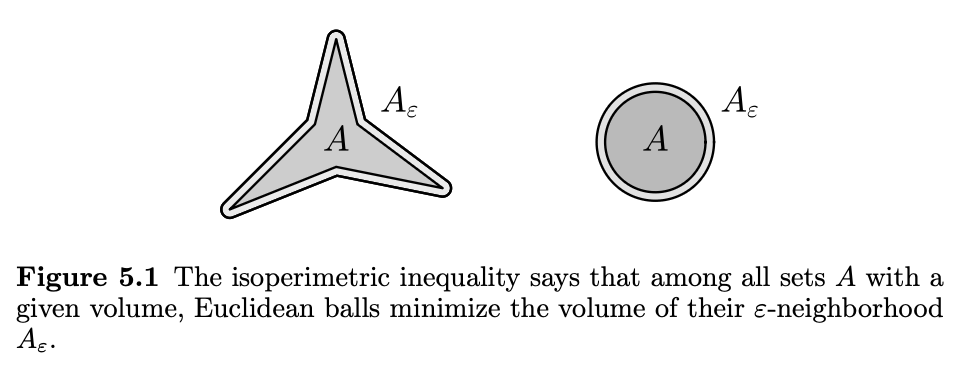
\includegraphics[width=0.8\textwidth]{Chapter 5/fig5-1.png}
\end{center}
\end{theorem}

A similar isoperimetric inequality holds for subsets on $S^{n - 1}$, and in this case the minimizers are the 
\underline{spherical caps} - neighborhoods of a single point. To state this principle, let $\sigma_{n - 1}$ 
denote the normalized are on the sphere $S^{n - 1}$ (The $n - 1$-dimensional Lebesgue measure).

\begin{theorem}[Isoperimetric inequality on the sphere]
\label{thm:5.1.5}
Let $\varepsilon > 0$. Then among all subsets $A \subset S^{n - 1}$ with given area $\sigma_{n - 1}(A)$, the 
spherical caps minimizer the area of the neighborhood $\sigma_{n - 1}(A_{\varepsilon})$, where 
\[ A_{\varepsilon} := \{ x \in \mathbb{R}^n: \ \exists y \in S^{n - 1} \text{ such that } 
\lVert x - y \rVert_{2} \leq \varepsilon \}. \]
\end{theorem}


\subsubsection{Blow-up of Sets on the Sphere}
The isoperimetric inequality leads to a remarkable and counterintuitive result: if a set $A$ covers at least 
half of the sphere in area, its $\varepsilon$-neighborhood $A_{\varepsilon}$ will cover most of the sphere. 
To simplify things in view of \cref{thm:5.1.3}, we'll operate on the sphere with radius $\sqrt{n}$.

\begin{lemma}[Blow-up]
\label{lem:5.1.6}
Let $A \subset \sqrt{n}S^{n - 1}$, and let $\sigma$ denote the normalized are on that sphere. If 
$\sigma(A) \geq 1/2$, then for every $t \geq 0$, 
\[ \sigma(A_t) \geq 1 - 2 \exp{(-ct^2)}. \]
\end{lemma}

\begin{proof}
Consider the hemisphere defined by the first coordinate:
\[ H := \{x \in \sqrt{n}S^{n - 1}: \ x_1 \leq 0 \}. \]
By assumption, $\sigma(A) \geq 1/2 = \sigma(H)$, hence the isoperimetric inequality (\cref{thm:5.1.5}) implies 
that 
\[ \sigma(A_t) \geq \sigma(H_t). \]
The neighborhood $H_t$ of the hemisphere $H$ is a spherical cap (a portion of a sphere cut off by a plane), 
and we could compute its area directly, but 
it is easier to use \cref{thm:3.4.5} instead, which states that a random vector $X \sim \mathrm{Unif}
(\sqrt{n}S^{n - 1})$ is subgaussian, and $\lVert X \rVert_{\psi_2} \leq C$. Since $\sigma$ is the uniform 
probability measure on the sphere, it follows that 
\[ \sigma(H_t) = P(X \in H_t). \]
Now, the definition of the neighborhood implies that 
\[ \{ x \in \sqrt{n}S^{n - 1}: \ x_1 \leq t / \sqrt{2} \} \subset H_t. \]
Thus
\[ \sigma(H_t) \geq P(X_1 \leq t / \sqrt{2}) \geq 1 - 2 \exp{(-ct^2)}. \]
The last inequality holds because $\lVert X_1 \rVert_{\psi_2} \leq \lVert X \rVert_{\psi_2} \leq C$. Then the 
lemma is proved because $\sigma(A_t) \geq \sigma(H_t)$.
\end{proof}

\begin{remark}[A more dramatic blow-up]
\label{rmk:5.1.7}
The $1/2$ value for the area in \cref{lem:5.1.6} was arbitrary, and can be replaced with any constant, or even 
an exponentially small quantity (Exercise 5.3)!
\end{remark}

\begin{remark}[A zero-one law]
\label{rmk:5.1.8}
The blow-up phenomenen we just saw can be quite counterintuitive at first. However, this is a typical p
phenomenon in high dimensions. It is similar to \textit{zero-one laws} in probability theory, which basically 
say that events influenced by many random variables tend to have probabilities zero or one.
\end{remark}


\subsubsection{Proof of Theorem 5.1.3}
WLOG, we can assume that $\lVert f \rVert_{\mathrm{Lip}} = 1$. Let $M$ denote the median of $f(X)$, which 
by definition satisfies 
\[ P(f(X) \leq M) \geq \frac{1}{2} \text{ and } P(f(X) \geq M) \geq \frac{1}{2}. \]
Consider the sublevel set 
\[ A := \{x \in \sqrt{n}S^{n - 1}: \ f(x) \leq M \}. \]
Since $P(X \in A) \geq \frac{1}{2}$, \cref{lem:5.1.6} implies that 
\[ P(X \in A_t) \geq 1 - 2 \exp{(-ct^2)}. \]
On the other hand, we claim that 
\[ P(X \in A_t) \leq P(f(X) \leq M + t). \]
Indeed, if $X \in A_t$ then $\lVert X - y \rVert_{2} \leq t$ for some point $y \in A$. By definition, 
$f(y) \leq M$. Since $f$ is Lipschitz with $\lVert f \rVert_{\mathrm{Lip}} = 1$, it follows that 
\[ f(X) \leq f(y) + \lVert X - y \rVert_{2} \leq M + t. \]
Combining the two bounds above, we conclude that 
\[ P(f(X) \leq M + t) \geq 1 - 2 \exp{(-ct^2)}. \]
Repeating the argument for $-f$, we obtain a similar bound for the probability that $f(x) \geq M - t$ (do). 
Combining the two, we get a similar bound for the probability that $|f(X) - M| \leq t$, and conclude that 
\[ \lVert f(X) - M \rVert_{\psi_2} \leq C. \]
Then we can replace the median by the mean, which follows by centering (\cref{lem:2.7.8}). Therefore the proof 
is complete. $\square$



% ----------5.2----------
\subsection{Concentration on Other Metric Measure Spaces}
We can extend concentration from the sphere to other spaces as well. The proof of \cref{thm:5.1.3} relied 
on two ingredients: 
\begin{enumerate}
	\item an isoperimetric inequality,
	\item a blow-up of its minimizers.
\end{enumerate}
There are not unique to the sphere - many spaces satusfy them hence we can derive similar concentration results.

\begin{remark}[]
\label{rmk:5.2.1}
Concentration keeps the mean, median, and $L^p$ norms close. Therefore, we can always replace the mean 
$\mathbb{E}[f(X)]$ with the median (Exercise 5.6), or, if the mean is nonnegative, with the $L^p$ norm for any 
$p \geq 1$, though the constant may depend on $p$ (Exercise 5.10).
\end{remark}


\subsubsection{Gaussian Concentration}
The \underline{Gaussian measure} of a Borel set $A \subset \mathbb{R}^n$ is defined as 
\[ \gamma_n(A) := P(X \in A) = \frac{1}{(2 \pi)^{n / 2}} \int_{A}^{} e^{-\lVert x \rVert_{2}^2 / 2} \ dx \]
where $X \sim N(0, I_n)$ is the standard normal random vector in $\mathbb{R}^n$.

\begin{theorem}[Gaussian isoperimetric inequality]
\label{thm:5.2.2}
Let $\varepsilon > 0$. Then among all sets $A \subset \mathbb{R}^n$ with given gaussian measure $\gamma_n(A)$, 
the half-spaces minimize the Gaussian measure of the neighborhood $\gamma_n(A_{\varepsilon})$.
\end{theorem}

\begin{theorem}[Gaussian concentration]
\label{thm:5.2.3}
Consider a random vector $X \sim N(0, I_n)$ and a Lipschitz function $f: \mathbb{R}^n \to \mathbb{R}$ (with 
respect to the Euclidean metric). Then 
\[ \lVert f(X) - \mathbb{E}[f(X)] \rVert_{\psi_2} \leq C \lVert f \rVert_{\mathrm{Lip}}. \]
\end{theorem}

\begin{example}[]
\label{ex:5.2.4}
Two special cases of \cref{thm:5.2.3} should already be familiar: 
\begin{enumerate}
	\item For linear functions $f$, it follows since $X \sim N(0, I_n)$ is subgaussian.
	\item For the Euclidean norm $f(x) = \lVert x \rVert_{2}$, it follows from norm concentration 
	(\cref{thm:3.1.1}).
\end{enumerate}
\end{example}


\subsubsection{Hamming Cube}
The method based on isoperimetry also works on the Hamming cube $(\{0, 1\}^n, d, \mathbb{P})$ 
(\cref{def:4.2.14}), where $d(x, y)$ is the normalized Hamming distance:
\[ d(x, y) = \frac{1}{n}|\{i: x_i \neq y_i\}|. \]
The measure $\mathbb{P}$ is the uniform probability measure on the cube: 
\[ \mathbb{P}(A) = \frac{|A|}{2^n} \text{ for any } A \subset \{0, 1\}^n. \]

\begin{theorem}[Concentration on the Hamming cube]
\label{ex:5.2.5}
Consider a random vector $X \sim \{0, 1\}^n$. Then for any function $f: \{0, 1\}^n \to \mathbb{R}$ we have 
\[ \lVert f(X) - \mathbb{E}[f(X)] \rVert_{\psi_2} \leq \frac{C \lVert f \rVert_{\mathrm{Lip}}}{\sqrt{n}}. \]
\end{theorem}


\subsubsection{Symmetric Group}
A similar result holds for the symmetric group $S_n$, a set of all $n!$ permutations of $\{1, \dots, n\}$. 
We can view the symmetric group as a metric measure space $(S_n, d, \mathbb{P})$, where $d(\pi, \rho)$ is the 
normalized Hamming distance - the fraction of the symbols on which permutations $\pi$ and $\rho$ differ:
\[ d(\pi, \rho) = \frac{1}{n} |\{i: \pi(i) \neq \rho(i)\}|. \]
The measure $\mathbb{P}$ is the uniform probability measure on $S_n$:
\[ \mathbb{P}(A) = \frac{|A|}{n!} \text{ for any } A \subset S_n. \]

\begin{theorem}[Concentration on the symmetric group]
\label{thm:5.2.6}
Consider a random permutation $X \sim \mathrm{Unif}(S_n)$ and a function $f: S_n \to \mathbb{R}$. Then 
\[ \lVert f(X) - \mathbb{E}[f(X)] \rVert_{\psi_2} \leq \frac{C \lVert f \rVert_{\mathrm{Lip}}}{\sqrt{n}}. \]
\end{theorem}


\subsubsection{Riemannian Manifolds with Strictly Positive Curvature}
(Feel free to skip this if not familiar with differential geometry)

A compact connected Riemannian manifold $(M, g)$ comes with the geodesic distance $d(x, y)$, which is the 
shortest length of a curve connecting the points. Then we can define a metric measure space $(M, d, \mathbb{P})$ 
where $\mathbb{P}$ is the uniform probability measure derived by normalizing the Riemannian volume. 

Let $c(M)$ denote the infimum of the Ricci curvature tensor over all tangent vectors. Assuming $c(M) > 0$, then 
it can be proved that 
\[ \lVert f(X) - \mathbb{E}[f(X)] \rVert_{\psi_2} \leq \frac{C \lVert f \rVert_{\mathrm{Lip}}}{\sqrt{c(M)}} \]
for any Lipschitz function $f: M \to \mathbb{R}$.

To give an example, $c(S^{n - 1}) = n - 1$. Then the above gives another approach for the concentration 
inequality of the sphere.


\subsubsection{Special Orthogonal Group}
The special orthogonal group $\mathrm{SO}(n)$ consists of all $n \times n$ orthogonal matrices with determinant 
1. We can treat it as a metric measure space $(\mathrm{SO}(n), \lVert \cdot \rVert_{F}, \mathbb{P})$, with 
distance given by the Frobenius norm $\lVert A - B \rVert_{F}$ and $\mathbb{P}$ as the uniform probability 
measure.

\begin{theorem}[Concentration on the special orthogonal group]
\label{thm:5.2.7}
Consider a random orthogonal matrix $X \sim \mathrm{Unif}(\mathrm{SO}(n))$ and a function $f: \mathrm{SO}(n) 
\to \mathbb{R}$. Then 
\[ \lVert f(X) - \mathbb{E}[f(X)] \rVert_{\psi_2} \leq \frac{C \lVert f \rVert_{\mathrm{Lip}}}{\sqrt{n}}. \]
\end{theorem}

The result above can be deduced from the concentration on general Riemannian manifolds.

\begin{remark}[Haar measure]
\label{rmk:5.2.8}
To generate a random orthogonal matrix $X \sim \mathrm{Unif}(\mathrm{SO}(n))$, one way is to start with an 
$n \times n$ Gaussian random matrix $G$ with $N(0, 1)$ independent entries, and compute its SVD 
$G = U \Omega V^T$. Then the matrix of left singular vectors is uniformly distributed in $\mathrm{SO}(n)$.

The uniform probability distribution on $\mathrm{SO}(n)$ is given by 
\[ \mu(A) := P(X \in A) \text{ for } A \subset \mathrm{SO}(n). \]
This is the unique rotation-invariant probaility measure on $\mathrm{SO}(n)$, called the 
\underline{Haar measure}.
\end{remark}


\subsubsection{Grassmannian}
The Grassmannian manifold $G_{n, m}$ consists of all $m$-dimensional subspaces of $\mathbb{R}^n$. When $m = 1$, 
it can be identified with the sphere $S^{n - 1}$. Therefore the concentration on the Grassmannian includes the 
concentration on the sphere. 

We can treat $G_{n, m}$ as a metric space $(G_{n, m}, d, \mathbb{P})$, where the distance between subspaces is 
given by the operator norm
\[ d(E, F) = \lVert P_E - P_F \rVert_{} \]
where $P_E$ and $P_F$ are the orthogonal projections onto the subspaces. The probability measure is the Haar 
measure (\cref{rmk:5.2.8}). A random subspace $E$ can hence be computed by computing the image of the random 
$n \times m$ Gaussian random matric with i.i.d. $N(0, 1)$ entries.

\begin{theorem}[Concentration on the Grassmannian]
\label{thm:5.2.9}
Consider a random subspace $X \sim \mathrm{Unif}(G_{n, m})$ and a function $f: G_{n, m} \to \mathbb{R}$. Then 
\[ \lVert f(X) - \mathbb{E}[f(X)] \rVert_{\psi_2} \leq \frac{C \lVert f \rVert_{\mathrm{Lip}}}{\sqrt{n}}. \]
\end{theorem}

\begin{proof}
The proof is a bit involved: Express the Grassmannian as the quotient via the special orthogonal group:
\[ G_{n, m} = \mathrm{SO}(n) / (\mathrm{SO}(m) \times \mathrm{SO}(n - m)) \]
and use the fact that concentration carries over to quotients.
\end{proof}


\subsubsection{Continuous Cube and Euclidean Ball}
\begin{theorem}[Concentration on the continuous cube and ball]
\label{thm:5.2.10}
Let $T$ be either the cube $[0, 1]^n$ or the ball $\sqrt{n}B_2^n$. Consider a random vector $X \sim 
\mathrm{Unif}(T)$ and a Lipschitz function $f; T \to \mathbb{R}$, where the Lipschitz norm is with respect 
to the Euclidean distance. Then 
\[ \lVert f(X) - \mathbb{E}[f(X)] \rVert_{\psi_2} \leq C \lVert f \rVert_{\mathrm{Lip}}. \]
\end{theorem}

\begin{proof}
Exercises 5.12 \& 5.13.
\end{proof}


\subsubsection{Densities of the Form \texorpdfstring{$e^{-U(x)}$}{}}
The push forward method from the previous section can be applied to many other distributions in $\mathbb{R}^n$. 
For example, suppose a random vector $X$ has a density of the form
\[ f(x) = e^{-U(x)} \]
for some function $U: \mathbb{R}^n \to \mathbb{R}$. For example, $X \sim N(0, I_n)$, the normal density gives 
$U(x) = \lVert x \rVert_{2}^2 + c$ where $c$ is constant (dependent on $n$ but not on $x$), and Gaussian 
concentration holds for $X$.

In general, we would expect that if $U$ has curvature at least like $\lVert x \rVert_{2}^2$, then there would be 
at least Gaussian concentration. As the theorem below shows, this depends on the Hessian of $U$:

\begin{theorem}[]
\label{thm:5.2.11}
Consider a random vector $X$ in $\mathbb{R}^n$ whose density has the form $e^{-U(x)}$ for some function 
$U: \mathbb{R}^n \to \mathbb{R}$. Assume there exists $\kappa > 0$ such that 
\[ \nabla^2 U(x) \succcurlyeq \kappa I_n \text{ for all } x \in \mathbb{R}^n. \]
Then any Lipschitz function $f: \mathbb{R}^n \to \mathbb{R}$ satisfies
\[ \lVert f(X) - \mathbb{E}[f(X)] \rVert_{\psi_2} \leq \frac{C \lVert f \rVert_{\mathrm{Lip}}}{\sqrt{\kappa}}. \]
\end{theorem}

\begin{proof}
THe proof uses semigroup methods, which are not covered in the text.
\end{proof}


\subsubsection{Random Vectors with Independent Bounded Coordinates}
There is a remarkable partial generalization of \cref{thm:5.2.10} for random vectors $X$ with independent 
coordinates that have arbitrary bounded distributions (not just uniform). By scaling, we can assume WLOG that 
$|X_i| \leq 1$.

\begin{theorem}[Talagrand concentration inequality]
\label{thm:5.2.12}
Consider a random vector in $\mathbb{R}^n$, 
$X = (X_1, \dots, X_n)$ whose coordinates are independent and satisfy $|X_i| \leq 1$ 
almost surely. Then for any Lipschitz function $f: [-1, 1]^n \to \mathbb{R}$, 
\[ \lVert f(X) - \mathbb{E}[f(X)] \rVert_{\psi_2} \leq C \lVert f \rVert_{\mathrm{Lip}}. \]
\end{theorem}



% ----------5.3----------
\subsection{Application: Johnson-Lindenstrauss Lemma}
Suppose we have $N$ data points in $\mathbb{R}^n$ where the dimension $n$ is very large. Can we reduce the 
dimension without losing the geometry of the data? The simplest way is to project onto a low-dimensional 
subspace 
\[ E \subset \mathbb{R}^n, \ \dim{(E)} := m \ll n, \]
see Figure 5.2 below. How shall we choose the subspace $E$, and how small should its dimension $m$ be?

\begin{center}
	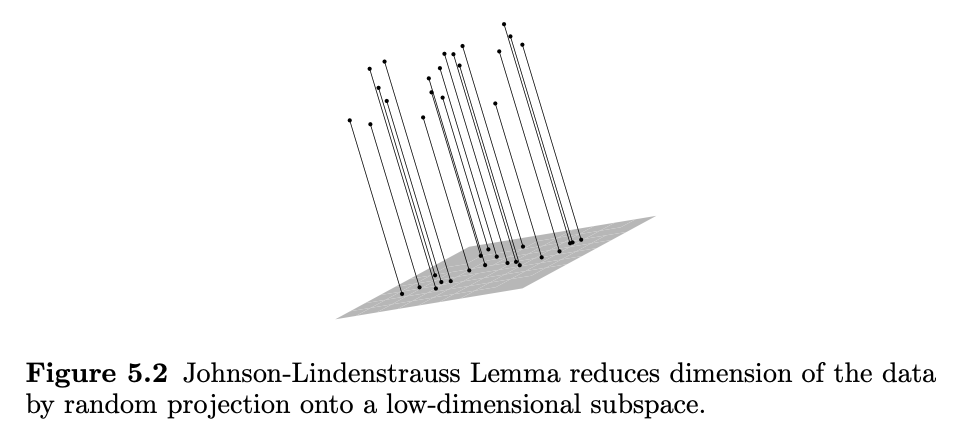
\includegraphics[width=0.8\textwidth]{Chapter 5/fig5-2.png}
\end{center}

The Johnson-Lindenstrauss Lemma states that the geometry of data is well preserved if we choose $E$ to be a 
\textit{random subspace} of dimension 
\[ m \asymp \log_{}{N}. \]
Here we say that $E$ is a random $m$-dimensional subspace in $\mathbb{R}^n$ uniformly distributed in $G_{n, m}$, 
i.e. 
\[ E \sim \mathrm{Unif}(G_{n,m}), \]
if $E$ is a random $m$-dimensional subspace of $\mathbb{R}^n$ whose distribution is rotation invariant, i.e. 
\[ P(E \in \mathcal{E}) = P(U(E) \in \mathcal{E}) \]
for any fixed subset $\mathcal{E} \in G_{n,m}$ and $n \times n$ orthogonal matrix $U$.

\begin{theorem}[Johnson-Lindenstrauss Lemma]
\label{thm:5.3.1}
Let $\mathcal{X}$ be a set of $N$ points in $\mathbb{R}^n$ and $\varepsilon > 0$. Assume that 
\[ m \geq C \varepsilon^{-2}\log_{}{N}. \]
Let $P$ be the orthogonal projection in $\mathbb{R}^n$ onto a random $m$-dimensional subspace $E \sim 
\mathrm{Unif}(G_{n, m})$. Then, with probability at least $1 - 2 \exp{(-c \varepsilon^2 m)}$, the scaled 
projection $Q = \sqrt{n/m}P$ is an approximate isometry on $\mathcal{X}$:
\[ (1 - \varepsilon)\lVert x - y \rVert_{2} \leq \lVert Qx - Qy \rVert_{2} 
\leq (1 + \varepsilon)\lVert x - y \rVert_{2} \texxt{ for all } x, y \in \mathcal{X}. \]
\end{theorem}
The proof will be based on concentration of Lipschitz functions on the sphere in Section 5.1 We 
use it to examine how the random projection $P$ acts on the fixed vector $x - y$, then take the union bound over 
all $N^2$ differences $x - y$.

\begin{lemma}[Random Projection]
\label{lem:5.3.2}
Let $P$ be a projection in $\mathbb{R}^n$ onto a random $m$-dimensional subspace $E \sim 
\mathrm{Unif}(G_{n,m})$. Fix any $z \in \mathbb{R}^n$ and $\varepsilon > 0$. Then,
\begin{enumerate}
	\item $(\mathbb{E}\left[ \lVert Pz \rVert_{2}^2 \right])^{1/2} = \sqrt{\frac{m}{n}} \lVert z \rVert_{2}$.
	\item With probability at least $1 - 2 \exp{(-c \varepsilon^2 m)}$, we have 
	\[ (1 - \varepsilon)\sqrt{\frac{m}{n}}\lVert z \rVert_{2} \leq \lVert Pz \rVert_{2} 
	\leq (1 + \varepsilon)\sqrt{\frac{m}{n}}\lVert z \rVert_{2}. \]
\end{enumerate}
\end{lemma}

\begin{proof}
Without loss of generality, we may assume that $\lVert z \rVert_{2} = 1$. Now switch the view. A random 
$m$-dimensional subspace $E$ can be obtained by randomly rotating some fixed subspace, such as the coordinate 
subspace $\mathbb{R}^m$. But instead of fixing $z$ and randomly rotate $\mathbb{R}^m$, we cna fix the the 
subspace $E = \mathbb{R}^m$ and randomly rotate $z$, which makes $z$ uniformly distributed on the sphere:
\[ z \sim \mathrm{Unif}(S^{n - 1}). \]
By rotation invariance, $Pz$ has the same distribution!

(a) Since $P$ is the projection onto the first $m$ coordinates in $\mathbb{R}^n$, 
\[ \mathbb{E}\left[ \lVert Pz \rVert_{2}^2 \right] = \mathbb{E}\left[ \sum_{i = 1}^{m} z_i^2 \right] 
= \sum_{i = 1}^{m}\mathbb{E}\left[ z_i^2 \right] = m \mathbb{E}\left[ z_1^2 \right], \]
because the coordinates $z_i$ of the random vector $z \sim \mathrm{Unif}(S^{n - 1})$ are identically 
distributed. To compute $\mathbb{E}\left[ z_1^2 \right]$, note that $\sum_{i = 1}^{n}z_i^2 = 1$. Taking 
expectations on both sides, we obtain 
\[ \sum_{i = 1}^{n}\mathbb{E}\left[ z_i^2 \right] = 1 \implies \mathbb{E}\left[ z_1^2 \right] = \frac{1}{n}. \]
Then, putting this into the equation above, we have 
\[ \mathbb{E}\left[ \lVert Pz \rVert_{2}^2 \right] = \frac{m}{n}. \]

(b) $x \mapsto \lVert Px \rVert_{2}$ is a Lipschitz function on $S^{n - 1}$ with Lipschitz norm bounded by 1. 
Then from Exercise 5.5, the concentration inequality gives 
\[ P \left( \left| \lVert Px \rVert_{2} - \sqrt{\frac{m}{n}} \right| \geq t \right) 
\leq 2 \exp{(-cnt^2)}. \]
(We replaced $\mathbb{E}\left[ \lVert x \rVert_{2} \right]$ by $(\mathbb{E}\left[ \lVert x \rVert_{2}^2 \right]^
{1/2})$ in the concentration inequality using \cref{rmk:5.2.1}). Choosing $t := \varepsilon \sqrt{m/n}$, we 
complete the proof.
\end{proof}

\begin{proof}[Proof of Johnson-Lindenstrauss Lemma]
Consider the difference set 
\[ \mathcal{X} - \mathcal{X} := \{ x - y: \ x, y \in \mathcal{X} \}. \]
We would like to show that, with required probability, the inequality
\[ (1 - \varepsilon)\lVert z \rVert_{2} \leq \lVert Qz \rVert_{2} \leq (1 + \varepsilon)\lVert z \rVert_{2} \]
holds for all $z \in \mathcal{X} - \mathcal{X}$. Since $Q = \sqrt{n/m}P$, this inequality is equivalent to 
\[ (1 - \varepsilon)\sqrt{\frac{m}{n}}\lVert z \rVert_{2} \leq \lVert Pz \rVert_{2} 
\leq (1 + \varepsilon)\sqrt{\frac{m}{n}}\lVert z \rVert_{2}. \]
For any fixed $z$, \cref{lem:5.3.2} states that the above holds with probability at least $1 - 2 \exp{(-c 
\varepsilon^2 m)}$. It remains to take a union bound over $z \in \mathcal{X} - \mathcal{X}$. It follows that 
the bound above holds simultaneously for all $z \in \mathcal{X} - \mathcal{X}$, with probability at least 
\[ 1 - |\mathcal{X} - \mathcal{X}| \cdot 2 \exp{(-c \varepsilon^2 m)} \geq 1 - N^2 \cdot 
2 \exp{(-c \varepsilon^2 m)}. \]
If $m \geq C \varepsilon^{-2} \log_{}{N}$ then this probability is at least $1 - 2 
\exp{(-c \varepsilon^2 m/2)}$, as claimed. Hence the proof is done.
\end{proof}

\begin{remark}[Non-adaptive, dimension-free]
\label{rmk:5.3.3}
A remarkable feature of the JL lemma is that the dimension reduction map $A$ is \textit{non-adaptive}, 
meaning it does not depend on the data. Note also that the ambient dimension $n$ of the data plays no role. With 
more toold, we will develop more advanced versions of the JH lemma (Exercise 9,37-9.39).
\end{remark}

\begin{remark}[Optimality]
The JL lemma makes such a striking dimension reduction from $N$ to $n = O(\log_{}{N})$. Can we go even smaller, 
say $n = o(\log_{}{N})$? Exercise 5.15 shows that we can't - the log dimension is the best we can do, even with 
nonlinear maps.
\end{remark}



% ----------5.4----------
\subsection{Matrix Bernstein Inequality}
We extend generalized concentration inequalities from sums of independent random variables to sums of 
independent random matrices. We'll make a matrix version of Bernstein inequality (\cref{thm:2.9.5}) by 
replacing random variables by random matrices, and absolute value by the operator norm. No need for 
independence of entries, rows, or columns within each random matrix!

\begin{theorem}[Matrix Bernstein inequality]
\label{thm:5.4.1}
Let $X_1, \dots, X_N$ be independent, mean zero, $n \times n$ symmetric random matrices, such that 
$\lVert X_i \rVert_{} \leq K$ almost surely for all $i$. Then for every $t \geq 0$, 
\[ P \left( \lVert \sum_{i = 1}^{N}X_i \rVert_{} \geq t \right) \leq 
2n \exp{\left( -\frac{t^2 / 2}{\sigma^2 + Kt / 3} \right)} \]
where $\sigma^2 = \lVert \sum_{i = 1}^{N} \mathbb{E}[X_i^2] \rVert_{}$ is the operator norm of the matrix 
variance of the sum.
\end{theorem}
We can rewrite the RHS of the inequality as the mixture of subgaussian and subexponential tail, like in the 
scalar Bernstein inequality:
\[ P \left( \lVert \sum_{i = 1}^{N}X_i \rVert_{} \geq t \right) \leq 
2n \exp{\left[ -c \cdot \min_{}\left( \frac{t^2}{\sigma^2}, \frac{t}{K} \right) \right]}. \]
The proof is similar to that of the scalar version: Repeat the MGF argument, swapping scalars with matrices. 
However, there is a big problem: Matrix multiplication is not commutative! Therefore we need some matrix 
calculus knowledge first.


\subsubsection{Matrix Calculus}
For an $n \times n$ symmetric matrix $X$, operations such as inversion or squaring only affect eigenvalues. 
For example, if the spectral decomposition of $X$ is $X = \sum_{i = 1}^{n} \lambda_i u_iu_i^T$, then
\[ X^{-1} = \sum_{i = 1}^{n} \frac{1}{\lambda_i}u_iu_i^T, \ 
X^2 = \sum_{i = 1}^{n} \lambda_i^2 u_iu_i^T, \ 
2I_n - 5X^3 = \sum_{i = 1}^{n} (2 - 5 \lambda_i^3)u_iu_i^T. \]
This suggest that for symmetric matrices, applying arbitrary functions on the matrices is equivalent to 
applying them to the eigenvalues:

\begin{definition}[Functions of matrices]
\label{def:5.4.2}
For a function $f: \mathbb{R} \to \mathbb{R}$ and an $n \times n$ symmetric matrix $X$ with spectral 
decomposition as above, define 
\[ f(X) := \sum_{i = 1}^{n} f(\lambda_i)u_iu_i^T. \]
\end{definition}
This definition agrees with matrix addition and multiplication, and with Taylor series (Exercise 5.16).

Of course, matrices can be compared with each other via a \underline{partial ordering}:
\begin{definition}[Loewner order]
\label{def:5.4.3}
We write $X \succcurlyeq 0$ if $X$ is a symmetric positive semidefinite matrix. We write $X \succeq Y$ and 
$Y \preceq X$ if $X - y \succeq 0$.
\end{definition}
This is a partial ordering because there are matrices for which neither $X \succeq Y$ nor $Y \succeq X$ holds.

\begin{proposition}[Simple properties of Loewner order]
\label{prop:5.4.4}
We have
\begin{enumerate}
	\item (Eigenvalue monotonicity) $X \preceq Y$ implies $\lambda_i(X) \leq \lambda_i(Y)$ for all $i$.
	\item (Trace monotonicity) For a (weakly) increasing function $f: \mathbb{R} \to \mathbb{R}$, 
	\[ X \preceq Y \implies \mathrm{tr}(f(X)) \leq \mathrm{tr}(f(Y)). \]
	\item (Operator norm) For any $a \geq 0$, 
	\[ \lVert X \rVert_{} \leq a \iff -aI_n \preceq X \preceq aI_n. \]
	\item (Upgrading scalar to matrix inequalities) For functions $f, g: \mathbb{R} \to \mathbb{R}$, 
	\[ f(x) \leq g(x) \forall x \text{ with } |x|\leq a \implies 
	f(X) \preceq g(X) \forall X \text{ with } \lVert X \rVert_{} \leq a. \]
\end{enumerate}
\end{proposition}

\begin{proof}
(a) If $X \preceq Y$, then $Y - X \succeq 0$ hence all eigenvalues of $Y - X$ are greater than equal to 0, 
and the result follows.

(b) The eigenvalues of $f(X)$ are $f(\lambda_i(X))$. The same can be said for $f(Y)$. By part (a) and the 
assumption, $f(\lambda_i(X)) \leq f(\lambda_i(Y))$. Summing these gives the result since the trace is the sum 
of the eigenvalues.

(c) From \cref{rmk:4.1.12}, $\lVert X \rVert_{} \leq a$ implies $u^T Xu \leq a$ for all unit vectors $u$. 
Therefore $u^T(aI_n - X)u \geq 0$ for all $u$, meaning $aI_n - X \succeq 0$, thus $X \preceq aI_n$. For the 
other inequality, again from \cref{rmk:4.1.12}, $u^T Xu \geq -a$ for all unit vectors $u$. Following the 
exact procedure above gives $X \succeq -aI_n$.

(d) By considering $g - f$, we can assume that $f = 0$. If $\lVert X \rVert_{} \leq a$, then all eigenvalues 
of $X$ satisfy $|\lambda_i| \leq a$, which implies $g(\lambda_i) \geq 0$ by assumption. So, by definition, 
$g(X)$ has nonnegative eigenvalues $g(\lambda_i)$ and so $g(X) \succeq 0$.
\end{proof}

\begin{remark}[Operator norm as matric absolute value]
\label{rmk:5.4.5}
(c) of \cref{prop:5.4.4} looks quite familiar... It is a matrix version of the basic fact about absolute 
values: for $x \in \mathbb{R}$, 
\[ |x| \leq a \iff -a \leq x \leq a. \]
This makes the operator norm $\lVert \cdot \rVert_{}$ a natural matrix version of the absolute value $|\cdot|$, 
and that's why it appeares in the matrix Bernstein inequality (\cref{thm:5.4.1}).
\end{remark}

\begin{remark}[Matrix monotonicity]
\label{rmk:5.4.6}
Can we strenghten trace monotonicity (\cref{prop:5.4.4} (b)) to matrix monotonicity, i.e.
\[ X \preceq Y \implies f(X) \preceq f(Y) \text{ for any weakly increasing } f: \mathbb{R} \to \mathbb{R}? \]
If $X$ and $Y$ commute, yes - but in general, no (Exercise 5.17). 

However, some functions, like $1/x$ and $\log_{}{x}$ on $[0, \infty)$, are \underline{matrix monotone}, meaning 
that the above holds even for non-commuting matrices:
\[ 0 \preceq X \preceq Y \implies X^{-1} \succeq Y^{-1} \succeq 0 \text{ and } \log_{}{X} \preceq \log_{}{Y} \]
whenever $X$ is invertible (Exercise 5.18).
\end{remark}


\subsubsection{Trace Inequalities}
Here is another identity that works for real numbers but not for matrices in general: $e^{x + y} = e^x e^y$ for 
scalars, but in Exercise 5.19, there are $n \times n$ symmetric matrices $X, Y$ such that 
\[ e^{X + Y} \neq e^X e^Y. \]
This is unfortunate, because when using the exponential moment method, we relied on this property to split 
the MGF via independence. 

Nevertheless, there are useful substitutes for the missing identity. In particular, this subsection covers two 
of them, both belonging to the rich family of \textit{trace inequalities}.

\begin{theorem}[Golden-Thompson inequality]
\label{thm:5.4.7}
For any $n \times n$ symmetric matrcies $A$ and $B$, 
\[ \mathrm{tr}(e^{A + B}) \leq \mathrm{tr}(e^A e^B). \]
\end{theorem}
Note that this does not hold for three or more matrices (we can find counterexamples)!

\begin{theorem}[Lieb inequality]
\label{thm:5.4.8}
Let $H$ be an $n \times n$ symmetric matrix. Define the function on matrices 
\[ f(X) := \mathrm{tr}(\exp{(H + \log_{}{X})}). \]
Then $f$ is concave on the space on PSD $n \times n$ symmetric matrices.
\end{theorem}

If $X$ is a random matrix, then Lieb and Jensen inequalities imply that 
\[ \mathbb{E}[f(X)] \leq f(\mathbb{E}[X]). \]
Applying this with $X = e^Z$, we obtain the following:

\begin{lemma}[Lieb inequality for random matrices]
\label{lem:5.4.9}
Let $H$ be a fixed $n \times n$ symmetric matrix and $Z$ be a random $n \times n$ symmetric matrix. Then 
\[ \mathbb{E}[\mathrm{tr}(\exp{(H + Z)})] \leq \mathrm{tr}(\exp{(H + \log_{}{\mathbb{E}[e^Z]})}). \]
\end{lemma}


\subsubsection{Proof of Matrix Bernstein Inequality}
(\textbf{Step 1: Reduction of MGF}) To bound the norm of the sum 
\[ S := \sum_{i = 1}^{N} X_i, \]
we need to control the largest and smallest eigenvalues of $S$. Consider the largest eigenvalue 
\[ \lambda_{\mathrm{max}}(S) := \max_{i} \lambda_i(S) \]
and note that 
\[ \lVert S \rVert_{} = \max_{i}|\lambda_i(S)| 
= \max_{}(\lambda_{\mathrm{max}}(S), \lambda_{\mathrm{max}}(-S)). \]
To bound $\lambda_{\mathrm{max}}(S)$, we'll use the exponential moment method again. Fix $\lambda > 0$. Via 
the typical procedure, 
\[ P(\lambda_{\mathrm{max}}(S) \geq t) 
= P(e^{\lambda \cdot \lambda_{\mathrm{max}}} \geq e^{\lambda t}) 
\leq e^{-\lambda t} \mathbb{E}[e^{\lambda \cdot \lambda_{\mathrm{max}}}]. \]
Then by \cref{def:5.4.2}, the eigenvalues of $e^{\lambda S}$ are $e^{\lambda \cdot \lambda_i(S)}$ so 
\[ E := \mathbb{E}[e^{\lambda \cdot \lambda_{\mathrm{max}}(S)}] 
= \mathbb{E}[\lambda_{\mathrm{max}}(e^{\lambda S})]. \]
Since the the eigenvalues of $e^{\lambda S}$ are all positive, the maximal eigenvalue is bounded by the sum of 
all eigenvalues, which is the trace. Therefore 
\[ E \leq \mathbb{E}[\mathrm{tr}(e^{\lambda S})]. \]

(\textbf{Step 2: Application of Lieb Inequality}) To use the Lieb inequality (\cref{lem:5.4.9}), we seperate 
the last term from the sum $S$:
\[ E \leq \mathbb{E}\left[ \mathrm{tr}\left( \exp{\left( \sum_{i = 1}^{N - 1} \lambda X_i 
+ \lambda X_N \right)} \right) \right]. \]
Condition on $(X_i)_{i = 1}^{N - 1}$ and apply \cref{lem:5.4.9} for the fixed matrix $H := \sum_{i = 1}^{N - 1} 
\lambda X_i$ and the random matrix $Z := \lambda X_N$. We get 
\[ E \leq \mathbb{E}[\mathrm{tr}(\exp{\left( \sum_{i = 1}^{N - 1} \lambda X_i 
+ \log_{}{\mathbb{E}[e^{\lambda X_N}]} \right)})]. \]
Then we continue the same procedure above: seperate $\lambda X_{N - 1}$ and apply \cref{lem:5.4.9}, and do the 
same thing for $N$ times to get 
\[ E \leq \mathrm{tr}\left( \exp{\left[ \sum_{i = 1}^{N} \log_{}{\mathbb{E}[e^{\lambda X_i}]} 
\right]} \right). \]

(\textbf{Step 3: MGF of the individual terms}) We'll bound the matrix-values MGF via the following lemma:
\begin{lemma}[Matrix MGF]
\label{lem:5.4.10}
Let $X$ be an $n \times n$ symmetric mean zero random matrix such that $\lVert X \rVert_{} \leq K$ almost 
surely. Then 
\[ \mathbb{E}[\exp{(\lambda X)}] \preceq \exp{(g(\lambda)\mathbb{E}[X^2]} 
\text{ where } g(\lambda) = \frac{\lambda^2 / 2}{1 - |\lambda|K / 3} \]
provided that $|\lambda| < 3 / K$.
\end{lemma}

\begin{proof}
First, we can bound the (scalar) exponential function by the first few terms via Taylor expansion:
\[ e^z \leq 1 + z + \frac{1}{1 - |z| / 3} \cdot \frac{z^2}{2}, \ |z| < 3. \]
(To get this inequality, write $e^Z = 1 + z + z^2 \sum_{p = 2}^{\infty} z^{p - 2} / p!$ and use the bound 
$p! \geq 2 \cdot 3^{p - 2}$). Next, apply this inequality to $z = \lambda x$. If $|x| \leq K$ and 
$|\lambda| < 3/K$ then we obtain 
\[ e^{\lambda x} \leq 1 + \lambda x + g(\lambda)x^2, \]
where $g(\lambda)$ is the same as how we defined in the statement.

Then we can upgrade this to a matrix inequality using \cref{prop:5.4.4} (d). If $\lVert X \rVert_{} \leq K$ and 
$|\lambda| < 3 / K$, then 
\[ e^{\lambda X} \preceq I + \lambda X + g(\lambda) X^2. \]
Taking expectations on both sides, since $\mathbb{E}[X] = 0$, 
\[ \mathbb{E}[e^{\lambda X}] \preceq I + g(\lambda) \mathbb{E}[X^2]. \]
To complete the proof of the lemma, let's use the inequality $1 + z \leq e^z$. We can transform this into a 
matrix inequality via \cref{prop:5.4.4} (d) and get $I + Z \preceq e^Z$ holds for all matrices $Z$, and in 
particular for $Z = g(\lambda)\mathbb{E}[X^2]$.
\end{proof}

(\textbf{Step 4: Completion of the proof}) Using \cref{lem:5.4.10}, we obtain 
\[ E \leq \mathrm{tr}\left( \exp{\left( \sum_{i = 1}^{N} \log_{}{\mathbb{E}[e^{\lambda X_i}]} 
\right)} \right) \leq \mathrm{tr}(\exp{(g(\lambda)Z)}), \text{ where } Z := \sum_{i = 1}^{N} \mathbb{E}[X_i^2]. \]where we used matric monotonicity of $\ln{x}$ (\cref{rmk:5.4.6}) to take logarithms on both sides, summed up 
the results, and used trace monotonicity (\cref{prop:5.4.4} (b)) to take traces of the exponential of both sides.

Since the trace of $\exp{(g(\lambda)Z)}$ is a sum of $n$ positive eigenvalues, it is bounded by $n$ times the 
maximum eigenvalue, hence 
\begin{align*}
	E 
	&\leq n \lambda_{\mathrm{max}}(\exp{(g(\lambda)Z)}) \\
	&= m \exp{(g(\lambda) \lambda_{\mathrm{max}}(Z))} \\
	&= n \exp{(g(\lambda) \lVert Z \rVert_{})} \quad (\text{Since } Z \succeq 0) \\
	&= n \exp{(g(\lambda)\sigma^2)} \quad (\text{By definition of } \sigma).
\end{align*}
Plugging in this bounde for $E = \mathbb{E}[e^{\lambda \cdot \lambda_{\mathrm{max}}(S)}]$ into the original 
equation gives
\[ P(\lambda_{\mathrm{max}}(S) \geq t) \leq n \exp{(-\lambda t + g(\lambda)\sigma^2)}. \]
The above is a bound that holds for any $\lambda > 0$ as long as $|\lambda| < 3/K$, so we can minimize it in 
$\lambda$. Better yet, instead of compuiting the exact minimum (which can be quite ugly), we can choose the 
following value: $\lambda = t / (\sigma^2 + Kt / 3)$, and substituting this value back gives 
\[ P(\lambda_{\mathrm{max}}(S) \geq t) \leq n \exp{\left( -\frac{t^2 / 2}{\sigma^2 + Kt / 3} \right)}. \]
Repeating the argument for $-S$, we will get the same bound as the above, and summing up the two bounds 
completes the proof. $\square$

\begin{remark}[Matrix Bernstein Inequality: expectation]
\label{rmk:5.4.11}
Matrix Bernstein inequality gives a high-probability bound. It can be turned into a simpler (but less 
informative) expectation bound in a standard way. Using \cref{thm:5.4.1} and the integrated tail formula 
(\cref{lem:1.6.1}), we can deduce that (Exercise 5.20)
\[ \mathbb{E}\left[ \lVert \sum_{i = 1}^{N} X_i \rVert_{} \right] 
\lesssim \lVert \sum_{i = 1}^{N} \mathbb{E}[X_i^2] \rVert_{}^{1/2} \sqrt{\log_{}{(2n)}} + K \log_{}{(2n)} \]
where the $\lesssim$ symbol hides an absolute constant factor. In the scalar case $(n = 1)$, an expectation 
bound is trivial: the variance of sum formula gives 
\[ \mathbb{E}\left[ \left| \sum_{i = 1}^{N} X_i \right| \right] 
\leq \left( \mathbb{E}\left[ \left| \sum_{i = 1}^{N} X_i \right|^2 \right] \right)^{1/2} 
= \left( \sum_{i = 1}^{N} \mathbb{E}[X_i^2] \right)^{1/2}. \]
\end{remark}

\begin{remark}[The logarithmic price]
For the equation in \cref{rmk:5.4.11}, the high-dimensional version differs the 1-dimensional one by just 
a logarithmic factor. This is a surprisingly small price for high dimensions! Moreover, this price is in 
essentially optimal - Exercise 5.28 gives an example of why we can't get rid of it.
\end{remark}


\subsubsection{Matrix Hoeffding and Khintchine Inequalities}
\begin{theorem}[Matrix Hoeffding inequality]
\label{thm:5.4.13}
Let $\varepsilon_1, \dots, \varepsilon_N$ be independent Rademacher random variables and $A_1, \dots A_N$ be 
any (fixed) symmetric $n \times n$ matrices. Then for any $t > 0$, 
\[ P \left( \lVert \sum_{i = 1}^{N} \varepsilon_i A_i \rVert_{} \geq t \right) 
\leq 2n \exp{\left( -\frac{t^2}{2 \sigma^2} \right)} \]
where $\sigma^2 = \lVert \sum_{i = 1}^{N} A_i^2 \rVert_{}$.
\end{theorem}

\begin{proof}
Exercise 5.21.
\end{proof}

\begin{theorem}[Matric Khintchine inequality]
\label{thm:5.4.14}
Let $\varepsilon_1, \dots, \varepsilon_N$ be independent Rademacher random variables and $A_1, \dots A_N$ be 
any (fixed) symmetric $n \times n$ matrices. Then for every $p \in [1, \infty)$, we have 
\[ \left( \mathbb{E}\left[ \lVert \sum_{i = 1}^{N} \varepsilon_i A_i \rVert_{}^p \right] \right)^{1/p} 
\leq C \sqrt{p + \log_{}{n}} \lVert \sum_{i = 1}^{N} A_i^2 \rVert_{}^{1/2}. \]
\end{theorem}

\begin{proof}
Exercise 5.22. Use the matrix Hoeffding inequality.
\end{proof}

\begin{remark}[Non-symmetric, rectangular matrices]
\label{rmk:5.4.15}
Matrix concentration inequalities easily extend to rectangular matrices using the \textit{Hermitian dilation} 
introduced in Exercise 4.14. Replace each matrix $X_i$ with the symmetric block matrix 
\[ \begin{bmatrix}
0 & X_i \\
X_i^T & 0 \\
\end{bmatrix} \]
and apply usual matrix concentration. We can get the matrix Bernstein (Exercise 5.23) and Khintchine (Exercise 
5.24) inequalities for rectangular matrices this way.
\end{remark}



% ----------5.5----------
\subsection{Application: Community Detection in Sparse Networks}
In section 4.5, the method of \textit{spectral clustering} was introduced, which is a basic method for 
community detection in networks. We showed that it works for relatively dense networks, where the expected 
average degree is $\gtrsim \sqrt{n}$. Now, using the matrix Bernstein inequality, we will show that spectral 
clustering actually works for much sparser networks, with an expected average degree as low as $O(\log_{}{n})$.

\begin{theorem}[Spectral clustering for sparse stochastic block model]
\label{thm:5.5.1}
Let $G \sim G(n, p, q)$ where $p = a/n, q = b/n$ and $b < a < 3b$. Assume that 
\[ (a - b)^2 \geq Ca \log_{}{n}. \]
Then, with probability at least 0.99, the spectral clustering algorithm identifies the communities of $G$ 
with 99\% accuracy, i.e. misclassifying at most $0.01n$ vertices.
\end{theorem}

\begin{proof}
We'll follow that same proof as that from Section 4.5, but with a sharper error bound.

\textbf{Step 1: Decomposition.} Again, let's split $A$ into the deterministic and random parts:
\[ A = D + R \text{ where } D = \mathbb{E}\left[ A \right]. \]
Before, the analysis is mostly on the deterministic matrix $D$, where the second largest eigenvector has $\pm 1$ 
coefficients representing community membership. Now we have to analyze the random part 
\[ R = A - \mathbb{E}\left[ A \right]. \]
Let's decompose it entry by entry, keeping symmetry in mind. We can write $R$ as a sum of independent, mean-zero 
random matrices $Z_{ij}$ that isolate entries $(i, j)$ and $(j, i)$:
\[ R = \sum_{i \leq j}^{}Z_{ij}, \text{ where } Z_{ij} = \begin{cases}
	R_{ij}(e_ie_j^T + e_je_i^T) $\text{ if } i < j, \\
	R_{ii}e_ie_i^T &\text{ if } i = j
\end{cases}. \]

\textbf{Step 2: Bounding the error}. Since $A_{ij} \in \{ 0, 1 \}$, 
\[ |R_{ij}| \leq 1 \implies \lVert Z_{ij} \rVert_{} = \lVert R_{ij} \rVert_{} \leq 1 \implies 
\lVert R_{ij}Z_{ij} \rVert_{} \leq 1. \]
Then by applying the matrix Bernstein inequality (\cref{rmk:5.4.11}) combined with Markov's inequality, we 
obtain with probability at least 0.99:
\[ \lVert R \rVert_{} \lesssim \sigma \sqrt{\log_{}{n}} + \log_{}{n} \text{ where } 
\sigma^2 = \lVert \mathbb{E}\left[ \sum_{i \leq j}^{} Z_{ij}^2 \right] \rVert_{}. \]
Let's compute $\sigma^2$. A quick check shows thaaht $Z_{ij}^2$ is a diagonal matrix:
\[ Z_{ij}^2 = \begin{cases}
	R_{ij}^2 (e_ie_i^T + e_je_j^T) &\text{ if } i < j, \\
	R_{ii}^2 e_ie_i^T &\text{ if } i = j
\end{cases}. \]
Then, by symmetry, 
\[ \sum_{i \leq j}^{}Z_{ij}^2 = \sum_{i \leq j}^{}R_{ij}^2 (e_ie_i^T + e_je_j^T) + 
\sum_{i}^{} R_{ii}^2 e_ie_i^T = \sum_{i = 1}^{n} \left( \sum_{j = 1}^{n} R_{ij}^2 \right) e_ie_i^T. \]
This is a diagonal matrix, and so is its expectation. Thus 
\[ \sigma^2 = \lVert \mathbb{E}\left[ \sum_{i \leq j}^{}Z_{ij}^2 \right] \rVert_{} = 
\max_{i = 1, \dots, n} \sum_{j = 1}^{n} \mathbb{E}\left[ R_{ij}^2 \right] \]
since the operator norm of a diagonal matrix is the maximal absolue value of its entries (Exercise 4.3 (b)). 
Recall that $R_{ij} = A_{ij} - \mathbb{E}\left[ A_{ij} \right]$. In the stochastic block model, $A_{ij}$ is 
either $\mathrm{Ber}(p)$ or $\mathrm{Ber}(q)$. So $\mathbb{E}\left[ R_{ij}^2 \right] = \mathrm{Var}(A_{ij}) 
\leq p$ since $p > q$. Thus 
\[ \sigma^2 \leq np = a, \]
and substituting this into the initial bound for $\lVert R \rVert_{}$, we get 
\[ \lVert R \rVert_{} \lesssim \sqrt{a \log_{}{n}} + \log_{}{n} \lesssim \sqrt{a \log_{}{n}} \]
because the assumption implies that $a \gtrsim \log_{}{n}$. 

\textbf{Step 3: Applying Davis-Kahan.} Let's apply \cref{thm:4.1.15} (see Exercise 4.16) to $D$ and $A$, 
focusing on the second largest eigenvalue. As we noted in Section 4.5.4, the seperation between $\lambda_2(D)$ 
of $D$ and the rest of the spectrum is
\[ \delta = \min_{}(\lambda_2(D), \lambda_1(D) - \lambda_2(D)) = \min_{}\left( \frac{p - q}{2}, q \right)n 
= \frac{a - b}{2} \]
since $a \leq 3b$ by assumption. Using the bound on $R$ from the end of Step 2, the Davis-Kahan inequality 
guarantees that for some $\theta \in \{ -1, 1 \}$, the distance between the \textit{unit} eigenvectors of $D$ 
and $A$ (denoted with bars) satisfies 
\[ \lVert \bar{u}_2(D) - \theta \bar{u}_2(A) \rVert_{2} \leq \frac{2 \lVert R \rVert_{}}{\delta} 
\leq \frac{C_1 \sqrt{a \log_{}{n}}}{a - b} < \frac{1}{10} \]
if we choose the constant $C$ in the assumption of the theorem to be large enough. Multiply both sides by 
$\sqrt{n}$ to get 
\[ \lVert u_2(D) - \theta u_2(A) \rVert_{2} \lesssim \frac{\sqrt{n}}{10}. \]
Since all coefficients of $u_2(D)$ are $\pm 1$ and correctly identify community membership, it follows that at 
least $99\%$ of the coefficients in $\theta u_2(A)_j$ have the same sign as $u_2(D)_j$, and thus correctly 
identify the community membership.
\end{proof}

\begin{remark}[Sparsity]
\label{rmk:5.5.2}
The sparsest graphs for which \cref{thm:5.5.1} is nontrivial have expected average degree
\[ \frac{n(p + q)}{2} = \frac{a + b}{2} \asymp \log_{}{n}, \]
That's way sparser than the bound of $O(\sqrt{n})$ that we have acheived previously (\cref{rmk:4.5.3})! 
\end{remark}



% ----------5.6----------
\subsection{Application: Covariance Estimation for General Distributions}
In Section 4.7, we learned how to estimate the covariance metrix of a subgaussian distribution in $\mathbb{R}^n$ 
from a sample of size $O(n)$. Now, we drop the subgaussian assumption, making this work for much broader 
distributions, even discrete ones. The trade-odd is just a logarithmic oversampling factor!

For noration, we denote the sample covariance matrix as 
\[ \Sigma_m = \frac{1}{m}\sum_{i = 1}^{m}X_i X_i^T. \]
If $X$ has zero mean, then $\Sigma$ is the covariance matrix of $X$, and $\Sigma_m$ is the sample covariance 
matrix.

\begin{theorem}[General covariance estimation]
\label{thm:5.6.1} 
Let $X$ be a random vector in $\mathbb{R}^n \ (n \geq 2)$. Assume that for some $K \geq 1$, 
\[ \lVert X \rVert_{2} \leq K (\mathbb{E}\left[ \lVert X \rVert_{2}^2 \right])^{1/2} \text{ almost surely.} \]
Then for every positive integer $m$, we have 
\[ \mathbb{E}\left[ \lVert \Sigma_m - \Sigma \rVert_{} \right] \leq C \left( 
\sqrt{\frac{K^2 n \log_{}{n}}{m}} + \frac{K^2 n \log_{}{n}}{m} \right) \lVert \Sigma \rVert_{}. \]
\end{theorem}

\begin{proof}
By \cref{prop:3.2.1} (b), we have $\mathbb{E}\left[ \lVert X \rVert_{2}^2 \right] = \mathrm{tr}(\Sigma)$, hence 
the condition in the theorem becomes 
\[ \lVert X \rVert_{2}^2 \leq K^2 \mathrm{tr}(\Sigma) \text{ almost surely. } \]
Apply the expected version of the matrix Bernstein inequality (\cref{rmk:5.4.11}) for the sum of i.i.d. mean 
zero random matrices $X_iX_i^T - \Sigma$ and get 
\[ \mathbb{E}\left[ \lVert \Sigma_m - \Sigma \rVert_{} \right] = 
\frac{1}{m} \mathbb{E}\left[ \lVert \sum_{i = 1}^{m} (X_iX_i^T - \Sigma) \rVert_{} \right] 
\lesssim \frac{1}{m} (\sigma \sqrt{\log_{}{n}} + M \log_{}{n}) \]
where 
\[ \sigma^2 = \lVert \sum_{i = 1}^{m} \mathbb{E}\left[ (X_iX_i^t - \Sigma)^2 \right] \rVert_{} 
= m \lVert \mathbb{E}\left[ (XX^T - \Sigma)^2 \right] \rVert_{} \]
and $M$ is any number chosen so that 
\[ \lVert XX^T - \Sigma \rVert_{} \leq M \text{ almost surely. } \]
To complete the proof, it remains to bound $\sigma^2$ and $M$.

Let's start with $\sigma^2$. By expanding the square, 
\[ \mathbb{E}\left[ (XX^T - \sigma)^2 \right] = \mathbb{E}\left[ (XX^T)^2 \right] - \Sigma^2 
\lesssim \mathbb{E}\left[ (XX^T)^2 \right]. \quad (*) \]
Furthermore, the assumption at the beginning of the proof gives 
\[ (XX^T)^2 = \lVert X \rVert_{}^2 XX^T \lesssim K^2 \mathrm{tr}(\Sigma) XX^T. \]
Taking expectations on both sides, we get 
\[ \mathbb{E}\left[ (XX^T)^2 \right] \lesssim K^2 \mathrm{tr}(\Sigma) \Sigma. \]
Substituting this bound into $(*)$, we get a bound for $\sigma^2$:
\[ \sigma^2 \leq K^2 m \mathrm{tr}(\Sigma) \lVert \Sigma \rVert_{}. \]


On the other hand, bounding $M$ is easier:
\begin{align*}
	\lVert XX^T - \Sigma \rVert_{} 
	&\leq \lVert X \rVert_{2}^2 + \lVert \Sigma \rVert_{} \quad \text{(By triangle inequality)} \\
	&\leq K^2 \mathrm{tr}(\Sigma) + \lVert \Sigma \rVert_{} \quad \text{(By assumption)} \\
	&\leq 2K^2 \mathrm{tr}(\Sigma) =: M. \quad (\lVert \Sigma \rVert_{} \leq \mathrm{tr}(\Sigma) \text{ and } 
	K \geq 1).
\end{align*}
Substitute the bounds for $\sigma$ and $M$ into the overall bound, we get 
\[ \mathbb{E}\left[ \lVert \Sigma_m - \Sigma \rVert_{} \right] \leq 
\frac{1}{m} \left( \sqrt{K^2m \mathrm{tr}(\Sigma) \lVert \Sigma \rVert_{}} \cdot \log_{}{n} 
+ 2K^2 \mathrm{tr}(\Sigma) \cdot \log_{}{n} \right). \]
Finally, plugging in the bound $\mathrm{tr}(\Sigma) \leq n \lVert \Sigma \rVert_{}$ completes the proof.
\end{proof}

\begin{remark}[Sample complexity]
\label{rmk:5.6.2}
\cref{thm:5.6.1} shows that for any $\varepsilon \in (0, 1)$, we can estimate the covariance matrix with a 
small relative error: 
\[ \mathbb{E}\left[ \lVert \Sigma_m - \Sigma \rVert_{} \right] \leq \varepsilon \lVert \Sigma \rVert_{}, \]
as long as the sample size is 
\[ m \asymp \varepsilon^{-2} n \log_{}{n}. \]
Compared to the sample complexity $m \asymp \varepsilon^{-2}n$ for subgaussan distributions (\cref{rmk:4.7.2}), 
dropping the subgaussian assumption costs just a small logarithmic oversampling factor! In general, this factor 
cannot be dropped (Exercise 5.28).
\end{remark}

\begin{remark}[Low-dimensional distributions]
\label{rmk:5.6.3}
At the end of proof of \cref{thm:5.6.1}, we used a rough bound $\mathrm{tr}(\Sigma) \leq n \lVert \Sigma 
\rVert_{}$. But instead, we can express the conclusion via the \textit{effective rank} of $\Sigma$:
\[ r = r(\Sigma) = \frac{\mathrm{tr}(\Sigma)}{\lVert \Sigma \rVert_{}} \]
and get a sharper bound 
\[ \mathbb{E}\left[ \lVert \Sigma_m - \Sigma \rVert_{} \right] \leq C \left( 
\sqrt{\frac{K^2 r \log_{}{n}}{m}} + \frac{K^2 r \log_{}{n}}{m} \right) \lVert \Sigma \rVert_{}. \]
It shows that a sample of size 
\[ m \asymp \varepsilon^{-2} r \log_{}{n} \]
is enough to estimate the covaraince matrix. Since $r \leq n$, this sample size is at least as small as the 
value that we had estimated above. It is even much smaller for \textit{approximately low-dimensional} 
distributions that concentrate near lower-dimensional subspaces.
\end{remark}

\begin{remark}[Effective and stable rank of a matrix]
\label{rmk:5.6.4}
What does the effective rank from \cref{rmk:5.6.3} really tell us about a PSD matrix $\Sigma$? TO get an idea, 
write it as the sum of eigenvalues divided by the largest one:
\[ r(\Sigma) = \frac{\sum_{i = 1}^{n} \lambda_i(\Sigma)}{\max_{i} \lambda_i(\Sigma)}. \]
This is always bounded by the actual rank (number of nonzero eigenvalues) and can be much smaller for 
``approximately" low-rank matrices - ones having only a few large eigenvalues. A related idea is the 
\textit{stable rank}, defined for any matrix $A$
\[ s(A) = \frac{\lVert A \rVert_{F}^2}{\lVert A \rVert_{}^2} 
= \frac{\sum_{i = 1}^{n} \sigma_i^2(A)}{\max_{i} \lambda_i(\sigma)} = r(A^T A) = r(AA^T) \]
where $\sigma_i$ denotes the singular values. Both are ``soft" versions of rank that are stable under small 
changes. For some more intuition, see Exercise 5.26.
\end{remark}

\begin{remark}[High-probability guarantees]
\label{rmk:5.6.5}
We covered expectation bounds, but our argument actually gives a more informative high-probability guarantee:
\[ \lVert \Sigma_m - \Sigma \rVert_{} \leq C \left( 
\sqrt{\frac{K^2 r (\log_{}{n} + u)}{m}} + \frac{K^2 r (\log_{}{n} + u)}{m}\right) \lVert \Sigma \rVert_{} \]
with probability at least $1 - 2e^{-u}$. Here $r = \mathrm{tr}(\Sigma) / \lVert \Sigma \rVert_{} \leq n$ is 
the effective rank (Exercise 5.26).
\end{remark}

\begin{remark}[Boundedness assumption]
\label{rmk:5.6.6}
The boundedness assumption in \cref{thm:5.6.1} might seem strong, but it cannot be dropped in general: if $X$ 
is isotropic but zero with high probability, the sample is likely to consist entirely of zeros, making 
covariance estimation impossible (Exercise 5.27). However, this assumption can still be relaxed (Exercise 6.34). 
In practice, it is usually enforced by truncation - dropping a small percentage of samples with the largest norm.
\end{remark}



% ----------5.7----------
\subsection{Extra notes}
There are lots of other concentration theorems not went over in the text. A very useful one is the McDiarmid 
inequality, which generalizes the Hoeffding inequality:

\begin{theorem}[McDiarmid inequality]
\label{thm:5.7.1}
Let $X = (X_1, \dots, X_N)$ be a random vector with independent entries. Let $f: \mathbb{R}^n \to \mathbb{R}$ 
be a measurable function. Assume that the value of $f(x)$ can change by at most $c_i > 0$ under an arbitrary 
change of a single coordinate of $x \in \mathbb{R}^n$. Then for any $t > 0$, 
\[ P(f(X) - \mathbb{E}[f(X)] \geq t) \leq \exp{\left( -\frac{2t^2}{\sum_{i = 1}^{N}c_i^2} \right)}. \]
\end{theorem}

\section{Quadratic Forms, Symmetrization, and Contraction}
This section concerns mostly with decoupling, concentration of quadratic forms, symmetrization, and contraction, 
which are a number of basic toold of high-dimensional probability.



% ----------6.1----------
\subsection{Decoupling}
We'll look at \underline{quadratic forms} of the form
\[ \sum_{i, j = 1}^{n} a_{ij} X_i X_j = X^T AX = \left\langle X, AX \right\rangle \]
where $A = (a_{ij})$ is an $n \times n$ coefficient matrix and $X = (X_1, \dots, X_n)$ is a random vector 
with independent coordinates. Such quadratic forms are known as \underline{chaos}.

We can compute the expectation of a chaos. If $X_i$ have zero means and unit variances, then 
\[ \mathbb{E}[X^T AX] = \sum_{i, j = 1}^{n} a_{ij} \mathbb{E}[X_i X_j] 
= \sum_{i = 1}^{n} a_{ii} = \mathrm{tr}(A). \]

However, establishing concentration on a chaos is harder, because the terms of the sum above are not 
independent. However, we can overcome this difficulty via \underline{decoupling}. We'll replace the quadratic 
form above with the bilinear form 
\[ \sum_{i, j = 1}^{n} a_{ij}  X_iX_j' = X^T AX' = \left\langle X, AX' \right\rangle,  \]
where $X' = (X_1', \dots, X_n')$ is an independent copy of $X$. Bilinear forms are easier to analyze than 
quadratic forms as they are linear in $X$. Therefore if we condition on $X'$, we may treat the bilinear form 
as a sum of independent random variables
\[ \sum_{i = 1}^{n} \left( \sum_{j = 1}^{n} a_{ij} X_j' \right) X_i = \sum_{i = 1}^{n} b_i X_i \]
with fixed coefficients $b_i$.

\begin{theorem}[Decoupling]
Let $A$ be an $n \times n$ diagonal free matrix, i.e. all diagonal entries are zero. Let $X$ be a random vector 
in $\mathbb{R}^n$ with independent mean zero coordinates, and let $X'$ be an independent copy. Then for every 
convex function $F: \mathbb{R} \to \mathbb{R}$, 
\[ \mathbb{E}[F(X^T AX)] \leq \mathbb{E}[F(4X^T AX')]. \]
\end{theorem}

\begin{proof}
We'll replace the chaos by a partial chaos, which we extend back to the original chaos later via Jensen's 
inequality.

(\textbf{Step 1: Randomly selecting a partial sum}) To specify a random subset of indices $I$, we'll use 
\underline{selectors} - independent Bernoulli random variables $\delta_1, \dots, \delta_n \sim_{iid} 
\mathrm{Ber}(1/2)$. We define the index set 
\[ I := \{ i: \delta_i = 1 \}. \]
Condition on $X$. Since by assumption $a_{ii} = 0$ and 
\[ \mathbb{E}[\delta_i(1 - \delta_j)] = \frac{1}{2} \cdot \frac{1}{2} = \frac{1}{4} \text{ for all } i \neq j \]
we may express the chaos as 
\[ X^T AX = \sum_{i \neq j}^{} a_{ij} X_iX_j 
= 4 \mathbb{E}_{\delta}\left[ \sum_{i \neq j}^{} \delta_i(1 - \delta_j) a_{ij} X_iX_j \right] 
= 4 \mathbb{E}_I \left[ \sum_{(i, j_ \in I \times I^C)}^{} a_{ij}X_iX_j \right]. \]
(In the expression above, the subscripts $\delta$ and $I$ indicate the source of randomness in the conditional 
expectations. Since $X$ is fixed, the expectations are taken over the random selection of $\delta$, or 
equivalently, the random index set $I$).

(\textbf{Step 2: Applying $F$}) 
\end{proof}


\section{Random Processes}

\section{Chaining}
This chapter concerns some of the central methods for bounding random processes $(X_t)$. We'll go over concepts 
such as chaining, VC theory, generic chaining methods, and bounds such as Talagrand's inequality and Chevet's 
inequality. We'll apply these to concepts such as Monto Carlo integration, empirical processes, and statistical 
learning theory.



% ----------8.1----------
\subsection{Dudley Inequality}
For a general Gaussian process $(X_t)_{t \in T}$, Sudakove inequality (\cref{thm:7.4.1}) gives a \textit{lower} 
bound on 
\[ \mathbb{E}\left[ \sup_{t \in T}X_t \right] \]
in terms of the metric entropy pf $T$. Now we'll go for an upper bound. Moreover, we generalize from Gaussian 
processes to subgaussian processes as well.

\begin{definition}[]
\label{def:8.1.1}
A random process $(X_t)_{t \in T}$ on a metric space $(T, d)$ has \underline{subgaussian increments} if there 
exists $K > 0$ such that 
\[ \lVert X_t - X_s \rVert_{\psi_2} \leq Kd(t, s) \text{ for all } t, s \in T. \]
\end{definition}

\begin{example}[Gaussian processes]
\label{ex:8.1.2}
Let $(X_t)_{t \in T}$ be a Gaussian process on some set $T$. It naturally defines a \textit{canonical metric} 
on $T$: 
\[ d(t, s) := \lVert X_t - X_s \rVert_{L^2}, \ t, s \in T, \]
as we explained earlier. With respect to this metric, $(X_t)_{t \in T}$ clearly has subgaussian increments, 
with some absolute constant $K$.
\end{example}

Here is another (trivial) example: Any random process can be made to have subgaussian increments by defining 
the metric as $d(t, s) := \lVert X_t - X_s \rVert_{\psi_2}$.

Now we give a bound on a general subgaussian random process in terms of the metric entropy:

\begin{theorem}[Dudley's integral inequality]
\label{thm:8.1.3}
Let $(X_t){t \in T}$ be a mean-zero random process on a metric space $(T, d)$ with subgaussian increments as in 
\cref{def:8.1.1}. Then 
\[ \mathbb{E}\left[ \sup_{t \in T}X_t \right] \leq CK \int_{0}^{\infty} 
\sqrt{\log_{}{\mathcal{N}(T, d, \varepsilon)}} \ d \varepsilon. \]
\end{theorem}

Before going to the proof's let's compare Dudley's inequality with Sudakov's inequality (\cref{thm:7.4.1}), 
which for Gaussian processes, says:
\[ \mathbb{E}\left[ \sup_{t \in T}X_t \right] \geq c \sup_{\varepsilon > 0}\varepsilon 
\sqrt{\log_{}{\mathcal{N}(T, d, \varepsilon)}}. \]
Figure 8.1 below shows both bounds: 
\begin{center}
	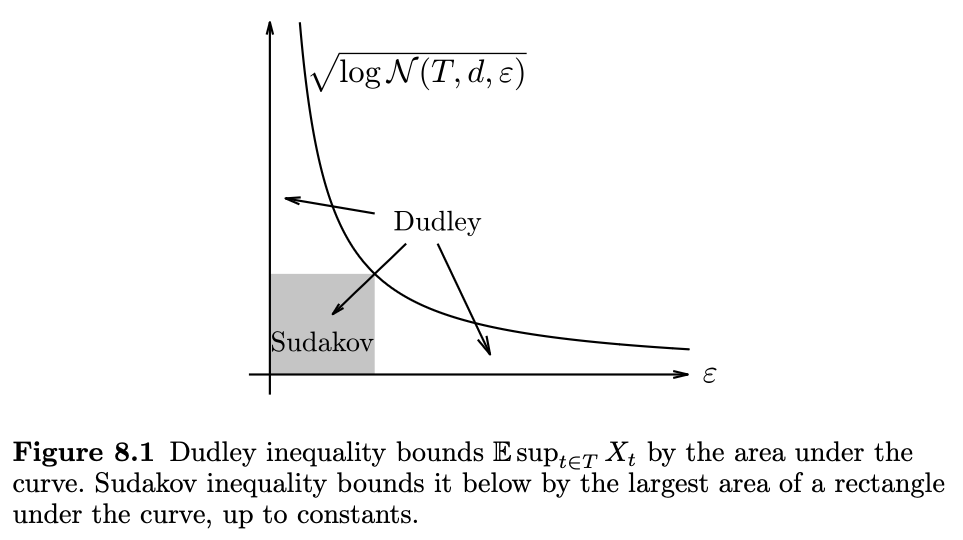
\includegraphics[width=0.8\textwidth]{Chapter 8/fig8-1.png}
\end{center}
There is a clear gap between the two bounds, and it turns out that metric entropy alone cannot close it - we 
will explore this later.

Dudley's inequality hints that $\mathbb{E}\left[ \sup_{t \in T}X_t \right]$ is a \textit{multiscale} quantity 
- to bound it, we need to look at $T$ across all scales $\varepsilon$. That's exactly how the proof works! But 
let's prove a discrete version using syadic scaled $\varepsilon = 2^{-k}$ like a Riemann sum, then move to the 
continuous version later.

\begin{theorem}[Discrete Dudley's inequality]
\label{thm:8.1.4}
Let $(X_t)_{t \in T}$ be a mean-zero random process on a metric space $(T, d)$ with subgaussian increments as 
from earlier. Then 
\[ \mathbb{E}\left[ \sup_{t \in T}X_t \right] \leq CK \sum_{k \in \mathbb{Z}}^{}2^{-k} 
\sqrt{\log_{}{\mathcal{N}(T, d, \varepsilon)}}. \]
\end{theorem}

The proof uses a technique called \textit{chaining}. It is a multi-scaled version of the $\varepsilon$-net 
argument that we did in \cref{thm:4.4.3} and \cref{thm:7.6.1}. In the $\varepsilon$-net argument, we approximate 
$T$ by an $\varepsilon$-net $\mathcal{N}$ so every point $t \in T$ is close to some $\pi(t) \in \mathcal{N}$, 
with $d(t, \pi(t)) \leq \varepsilon$. Then the increment condition gives 
\[ \lVert X_t - X_{\pi(t)} \rVert_{\psi_2} \leq K \varepsilon. \]
This leads to 
\[ \mathbb{E}\left[ \sup_{t \in T}X_t \right] \leq \mathbb{E}\left[ \sup_{t \in T}X_{\pi(t)} \right] 
+ \mathbb{E}\left[ \sup_{t \in T}(X_t - X_{\pi(t)}) \right]. \]
We can handle the first term via union bound over $|\mathcal{N}| = \mathcal{N}(T, d, \varepsilon)$ points 
$\pi(t)$. However, the second term is unclear (if we were to use union bound) since there is both $t$ and 
$\pi(t)$ in the supremum. To fix this, we don't stop at one net, but choose smaller and smaller $\varepsilon$ 
to get better approximations $\pi_1(t), \pi_2(t), \dots$ to $t$ with finer nets. This is the idea behind 
\textit{chaining}.

\begin{proof}[Proof of \cref{thm:8.1.4}]
\textbf{Step 1: Chaining setup.} Without loss of generality, we may assume that $K = 1$ (because of $C$) and 
$T$ is finite (\cref{rmk:7.2.1}). Define the dyadic scale 
\[ \varepsilon_k = 2^{-k}, \ k \in \mathbb{Z} \]
and choose $\varepsilon_k$-nets $T_k$ of $T$ so that 
\[ |T_k| = \mathcal{N}(T, d, \varepsilon_k). \]
Only a part of the dyadic scale will be needed. Since $T$ is finite, there exists a small enough number 
$\kappa \in \mathbb{Z}$ (defining the coarsest net) and a large enough number $K \in \mathbb{Z}$ (defining the 
finest net), such that 
\[ T_{\kappa} = \{t_0\} \text{ for some } t_0 \in T, \ T_K = T. \]
For a point $t \in T$, let $\pi_l(t)$ denote a closest point in $T_k$, so we have 
\[ d(t, \pi_k(t)) \leq \varepsilon_k. \]
Since $\mathbb{E}\left[ X_{t_0} \right] = 0$ by assumption, 
\[ \mathbb{E}\left[ \sup_{x \in T}X_t \right] = \mathbb{E}\left[ \sup_{x \in T}(X_t - X_{t_0}) \right]. \]
Let's write $X_t - X_{t_0}$ as a telescoping sum, walking from $t_0$ to $t$ along a chain (aha!) of points 
$\pi_k(t)$ that mark progressively finer approximations of $t$:
\[ X_t - X_{t_0} = (X_{\pi_{\kappa}(t)} - X_{t_0}) + (X_{\pi_{\kappa + 1}(t)} - X_{\pi_{\kappa}(t)}) 
+ \cdots + (X_t - X_{\pi_{K}(t)}), \]
see Figure 8.2 below for an illustration.
\begin{center}
    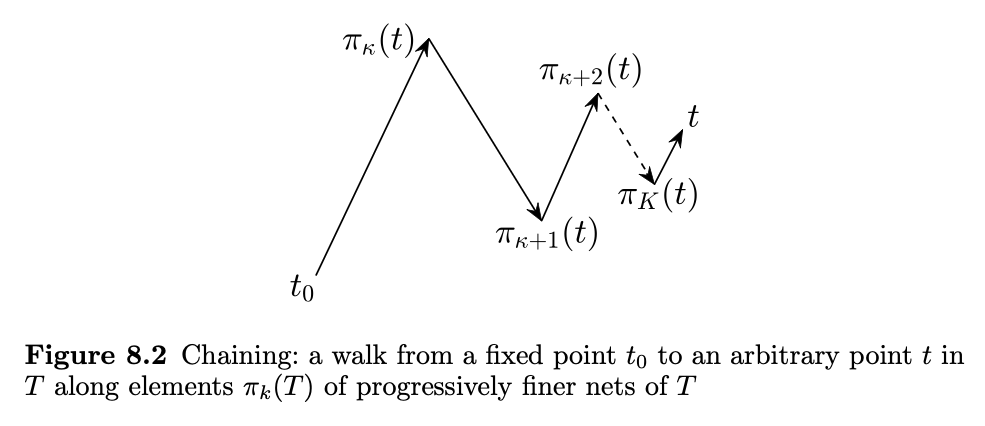
\includegraphics[width=0.8\textwidth]{Chapter 8/fig8-2.png}
\end{center}
The first and last terms of this sum are zero by our definition earlier, so we have 
\[ X_t - X_{t_0} = \sum_{k = \kappa + 1}^{K} (X_{\pi_k(t)} - X_{\pi_{k - 1}(t)}). \]
Since the supremum of the sum is bounded by the sum of the suprema, we get 
\[ \mathbb{E}\left[ \sup_{t \in T}(X_t - X_{t_0}) \right] \leq 
\sum_{k = \kappa + 1}^{K} \mathbb{E}\left[ \sup_{t \in T}(X_{\pi_k(t)} - X_{\pi_{k - 1}(t)}) \right]. \]

\textbf{Step 2: Controlling the increments.} In the equation above, it looks like we are taking the supremum 
over all of $T$ in each summand, but really it is over the smaller set of pairs $(\pi_k(t), \pi_{k - 1}(t))$. 
The number of such pairs is 
\[ |T_k| \cdot |T_{k - 1}| = |T_k|^2, \]
A number that we can control via covering numbers from above. Moreover, for a fixed $t$, we can bound the 
increments in step 1 like this: 
\begin{align*}
	\lVert X_{\pi_k(t)} - X_{\pi_{k - 1}(t)} \rVert_{\psi_2} 
	&\leq d(\pi_k(t), \pi_{k - 1}(t)) \quad \text{(By \cref{def:8.1.1})} \\ 
	&\leq d(\pi_k(t), t) + d(t, \pi_{k - 1}(t)) \quad \text{(By triangle inequality)} \\
	&\leq \varepsilon_k + \varepsilon_{k - 1} \quad \text{(By definition of )} \pi_k(t) \\
	&\leq 2 \varepsilon_{k - 1}.
\end{align*}
Recall from \cref{prop:2.7.6} that the expected maximum of $N$ subgaussian random variables is at most 
$CL \sqrt{\log_{}{N}}$, where $L$ is the largest $\psi_2$ norm. We can use this to bound each term: 
\[ \mathbb{E}\left[ \sup_{t \in T}(X_{\pi_k(t)} - X_{\pi_{k - 1}(t)}) \right] 
\leq C \varepsilon_{k - 1} \sqrt{\log_{}{|T_k|}}. \]

\textbf{Step 3: Summing up the increments.} We have shown that 
\[ \mathbb{E}\left[ \sup_{t \in T}(X_t - X_{t_0}) \right] 
\leq C \sum_{k = \kappa + 1}^{K} \varepsilon_{k - 1} \sqrt{\log_{}{|T_k|}}. \]
Now plug in the values $\varepsilon_k = 2^{-k}$ and the bounds on $|T_k|$, we get 
\[ \mathbb{E}\left[ \sup_{t \in T}(X_t - X_{t_0}) \right] 
\leq C_1 \sum_{k = \kappa + 1}^{K} 2^{-k} \sqrt{\log_{}{\mathcal{N}(T, d, 2^{-k})}}. \]
Hence the theorem is proved.
\end{proof}

Let's now go for the proof for the integral form of Dudley's inequality.

\begin{proof}[Proof of Dudley's integral inequality (\cref{thm:8.1.3})]
To convert the sum from the discrete form into an integral, we express $2^{-k}$ as 
$2 \int_{2^{-k-1}}^{2^{-k}}  \ d \varepsilon$. Then 
\[ \sum_{k \in \mathbb{Z}}^{} 2^{-k} \sqrt{\log_{}{\mathcal{N}(T, d, 2^{-k})}} = 
2 \sum_{k \in \mathbb{Z}}^{} \int_{2^{-k-1}}^{2^{-k}} \sqrt{\log_{}{\mathcal{N}(T, d, 2^{-k})}} \ 
d \varepsilon. \]
Within the limits of the integral, $2^{-k} \geq \varepsilon$, hence $\log_{}{\mathcal{N}(T, d, 2^{-k})} 
< \log_{}{\mathcal{N}(T, d, 2^{-k})}$ and the sum is bounded by 
\[ 2 \sum_{k \in \mathbb{Z}}^{} \int_{2^{-k-1}}^{2^{-k}} \sqrt{\log_{}{\mathcal{N}(T, d, \varepsilon)}} \ 
d \varepsilon = 2 \int_{0}^{\infty} \sqrt{\log_{}{\mathcal{N}(T, d, \varepsilon)}} \ d \varepsilon, \]
and the proof is complete.
\end{proof}

Actually, the discrete and integral Dudley inequalities are equivalent (Exercise 8.3).


\subsubsection{Variations and Examples}
\begin{remark}[Dudley's inequality: supremum of increments]
\label{rmk:8.1.5}
A quick look at the proof shows that chaining actually gives 
\[ \mathbb{E}\left[ \sup_{t \in T}|X_t - X_{t_0}| \right] \leq CK 
\int_{0}^{\infty} \sqrt{\log_{}{\mathcal{N}(T, d, \varepsilon)}} \ d \varepsilon \]
for any fixed $t \in T$. We can combine with the same bound for $X_s - X_{t_0}$, then use the triangle 
inequality to get 
\[ \mathbb{E}\left[ \sup_{t, s \in T}|X_t - X_s| \right] \leq CK 
\int_{0}^{\infty} \sqrt{\log_{}{\mathcal{N}(T, d, \varepsilon)}} \ d \varepsilon. \]
\end{remark}

\begin{remark}[Dudley's inequality: a high-probability bound]
\label{rmk:8.1.6}
Dudley's inequality gives only an expectation bound, but chaining actually gives a high-probability bouind. 
Assuming $T$ is finite (avoid measurability issues), for every $u \geq 0$, the bound 
\[ \sup_{t, s \in T} |X_t - X_s| \leq CK \left[ \int_{0}^{\infty} \sqrt{\log_{}{\mathcal{N}(T, d, \varepsilon)}} 
\ d \varepsilon + u \cdot \mathrm{diam}(T) \right] \]
holds with probability at least $1 - 2 \exp{(-u^2)}$ (Exercise 8.1). For Gaussian processes, this also follows 
directly from Gaussian concentration (Exercise 8.2).
\end{remark}

\begin{remark}[Limits of Dudley integral]
\label{rmk:8.1.7}
Even though the Dudley integral goes over $[0, \infty]$, we can cap it at the diameter of $T$, since for 
$\varepsilon > \mathrm{diam}(T)$, a single $\varepsilon$-ball covers $T$ and so 
\[ \mathcal{N}(T, d, \varepsilon) = 1 \implies \log_{}{\mathcal{N}(T, d, \varepsilon)} = 0. \]
Thus 
\[ \mathbb{E}\left[ \sup_{t \in T}X_t \right] \leq CK \int_{0}^{\mathrm{diam}(T)} 
\sqrt{\log_{}{\mathcal{N}(T, d, \varepsilon)}} \ d \varepsilon. \]
\end{remark}

If we apply Dudley's inequality for the canonical Gaussian process $\left\langle g, t \right\rangle$, just 
like we did with Sudakov's inequality in \cref{cor:7.4.2}, we get the following:

\begin{theorem}[Dudley's inequality in \texorpdfstring{$\mathbb{R}^n$}{}]
\label{thm:8.1.8}
The Gaussian width of any bounded set $Y \subset \mathbb{R}^n$ satisfies 
\[ w(T) \leq C \int_{0}^{\infty} \sqrt{\log_{}{\mathcal{N}(T, \varepsilon)}} \ d \varepsilon, \]
where $\mathcal{N}(T, \varepsilon)$ is the smallest number of Euclidean balls with radius $\varepsilon$ and 
centers in $T$ that cover $T$.
\end{theorem}

\begin{example}[Dudley's inequality is sharp for the Euclidean ball]
\label{ex:8.1.9}
Let's test Dudley's inequality for the unit Euclidean ball $T = B_2^n$. From \cref{cor:4.2.11}, 
\[ \mathcal{N}(B_2^n, \varepsilon) \begin{cases}
	\leq (3 / \varepsilon)^n &\text{ for } \varepsilon \in (0, 1], \\
	= 1 &\text{ for } \varepsilon > 1
\end{cases}. \]
Then 
\[ w(B_2^n) \lesssim \int_{0}^{1} \sqrt{n \log_{}{(3 / \varepsilon)}} \ d \varepsilon \lesssim \sqrt{n}. \]
This is in fact optimal: as we know from \cref{ex:7.5.6}, $w(B_2^n) \asymp \sqrt{n}$.
\end{example}

\begin{remark}[Dudley's inequality can be loose - but not too loose]
\label{rmk:8.1.10}
In general, Dudley integral can overestimate the Gaussian width. Here is a bad example: 
\[ T = \left\{ \frac{e_k}{\sqrt{1 + \log_{}{k}}}, \ k = 1, \dots, n \right\} \]
with $e_k$ being the standard basis in $\mathbb{R}^n$. From exercise 8.4, we can see that 
\[ w(T) = O(1) \text{ while } \int_{0}^{\infty} \sqrt{\log_{}{\mathcal{N}(T, d, \varepsilon)}} \ d \varepsilon 
\to \infty \]
as $n \to \infty$. However, the good news:
\begin{enumerate}
	\item Dudley equality is tight up to a logarithmic factor (Exercise 8.5);
	\item We will use chaining to remove that logarithmic factor in Section 8.5.
\end{enumerate}
\end{remark}


% ----------8.2----------
\subsection{Application: Empirical Processes}



% ----------8.3----------
\subsection{VC Dimension}
VC dimensions measures how complex a class of Boolean functions is, where a Boolean function is a map 
$f: \omega \to \{0, 1\}$ on some set $\omega$, and we are looking at some collection $\mathcal{F}$ of these.

\begin{definition}[]
\label{def:8.3.1}
A subset $\Lambda \subseteq \Omega$ is \underline{shattered} by a class of boolean functions $\mathcal{F}$ if, 
for any possible binary labeling $g: \Lambda \to \{0, 1\}$, there is some function $f \in \mathcal{F}$ that 
matches it on $\Lambda$. Formally, this means the restriction of $f$ onto $\Lambda$ is $g$, i.e. 
$f(x) = g(x) \text{ for all } x \in \Lambda$.

The \underline{Vapnik-Chervonenkis dimension (VC dimension)} of $\mathcal{F}$, denoted 
$\mathrm{vc}(\mathcal{F})$, is the largest cardinality of a subset $\Lambda \subseteq \Omega$ that is shattered. 
If there is no largest one, then $\mathrm{vc}(\mathcal{F}) = \infty$.
\end{definition}

Let's go through a few examples to make the definition clearer:

\begin{example}[Intervals]
\label{ex:8.3.2}
Let $\mathcal{F}$ consist of the indicators of all closed intervals in $\mathbb{R}$:
\[ \mathcal{F} = \left\{ \mathbf{1}_{[a, b]}: \ a, b \in \mathbb{R}, \ a \leq b \right\}. \]
We claim that 
\[ \mathrm{vc}(F) = 2. \]

We first show that $\mathrm{vc}(\mathcal{F}) \geq 2$ by finding a two-point set $\Lambda \subset \mathbb{R}$ 
that is shattered by $\mathcal{F}$. Take, for example, $\Lambda = 3, 5$. There are four possible binary 
labelings $g: \Lambda \to \{0, 1\}$ on this set, and each one can be obtained by restricting some interval 
indicator $f = \mathbf{1}_{[a, b]}$ ontp $\Lambda$. For example, $g(3) = 1, g(5) = 0$ comes from 
$f = \mathbf{1}_{[2, 4]}$. The other three cases are shown in Figure 8.5, so $\Lambda$ is indeed shattered by 
$\mathcal{F}$.

\begin{center}
    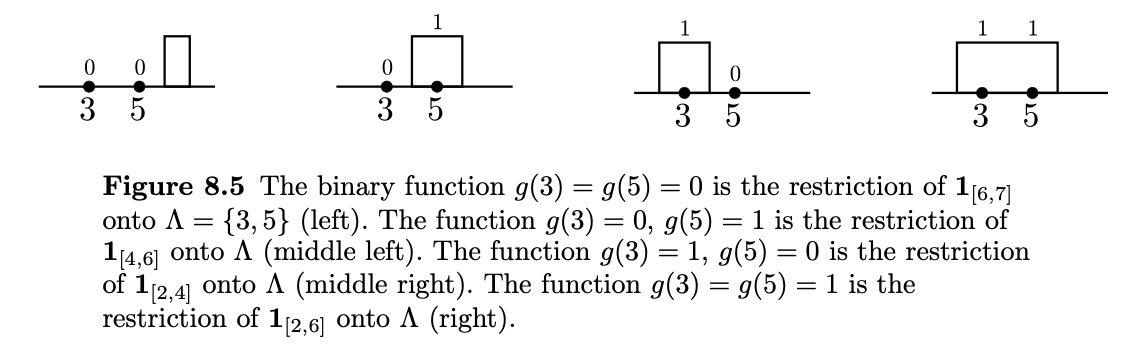
\includegraphics[width=0.8\textwidth]{Chapter 8/fig8-5.png}
\end{center}

To prove $\mathrm{vc}(\mathcal{F}) < 3$, we need to show that no three-point set $\Lambda = \{p, q, r\}$ can 
be shattered by $\mathcal{F}$. To see this, assume $p < q < r$ and consider the labeling $g(p) = 1, g(q) = 0, 
g(r) = 1$. Then $g$ cannot be a restriction of any indicator interval onto $\Lambda$ (it is not linearly 
seperable).
\end{example}



% ----------8.4----------
\subsection{Application: Statistical Learning Theory}



% ----------8.5----------
\subsection{Generic Chaining}



% ----------8.6----------
\subsection{Chevet Inequality}




\section{Deviations of Random Matrices on Sets}
The main question in this chapter is: How does an $m \times n$ matrix act on a general set $t \subset 
\mathbb{R}^n$? 



% ----------9.1----------
\subsection{Matrix Deviation Inequality}
Take an $m \times n$ random matrix $X$ with independent, isotropic, and subgaussian rows. The concentration of 
the norm (\cref{thm:3.1.1}) tells us that for any fixed vector $x \in \mathbb{R}^n$, the approximation 
\[ \lVert Ax \rVert_{2} \approx \sqrt{m}\lVert x \rVert_{2} \]
holds with high probability.

Let's ask something more general: Is it true that with high probability, the equation above holds 
\textit{simultaneously} for many vectors $x \in \mathbb{R}^n$? To quantify how many, pick some bounded set 
$T \subset \mathbb{R}^n$ and ask if the approximation holds simultaneously for all $x \in T$. It turns out that 
the maximal error is about $\gamma(T)$, the Gaussian complexity of $T$.

\begin{theorem}[Matrix deviation inequality]
\label{thm:9.1.1}
Let $A$ be an $m \times n$ random matrix with independent, isotropic and subgaussian rows $A_i$. Then for any 
subset $T \subset \mathbb{R}^n$, 
\[ \mathbb{E}\left[ \sup_{x \in T}\left| \lVert Ax \rVert_{2} - \sqrt{m}\lVert x \rVert_{2} \right| \right] 
\leq CK^2 \gamma(T), \]
where $\gamma(T)$ is the Gaussian complexity from Section 7.5.3, defined as 
\[ \gamma(T) = \mathbb{E}\left[ \sup_{x \in T}|\left\langle g, x \right\rangle| \right], \ g \sim N(0, I_n), \]
and $K = \max_{i} \lVert A_i \rVert_{\psi_2}$.
\end{theorem}

The plan is to deduce this from Talagrand's comparison inequality (\cref{cor:8.5.8}). To do that, we just have 
to check the random process 
\[ Z_x := \lVert Ax \rVert_{2} - \sqrt{m}\lVert x \rVert_{2} \]
indexed by vectors $x \in \mathbb{R}^n$ has subgaussian increments. Here is the claim:

\begin{theorem}[Subgaussian increments]
\label{thm:9.1.2}
Let $A$ be an $m \times n$ random matrix with independent, isotropic and subgaussian rows $A_i$. Then the random 
process $Z_x$ defined above has subgaussian increments: 
\[ \lVert Z_x - Z_y \rVert_{\psi_2} \leq CK^2 \lVert x - y \rVert_{2} \text{ for all } x, y \in \mathbb{R}^n, \]
here $K = \max_{i} \lVert A_i \rVert_{\psi_2}$.
\end{theorem}

Once we have proved this theorem, we plug it into Talagrand's comparison inequality (Exercise 8.37 (a)) and get 
\[ \mathbb{E}\left[ \sup_{x \in T} |Z_x| \right] \leq CK^2 \gamma(T) \]
which directly gives \cref{thm:9.1.1}. So, all we have to do is prove \cref{thm:9.1.2} - and it is in fact 
easier since it's for fixed $x$ and $y$.

\begin{proof}[Proof of \cref{thm:9.1.2}]
This argument will be a bit longer than usual, so we'll (hopefully) make it easier by starting with simpler 
cases and building up from there.

\textbf{Step 1: Unit vector $x$ and zero vector $y$.} If $\lVert x \rVert_{2} = 1$ and $y = 0$, the inequality 
in the theorem statement becomes 
\[ \left\lVert \lVert Ax \rVert_{2} - \sqrt{m} \right\rVert_{\psi_2} \leq CK^2. \]
The random vector $Ax \in \mathbb{R}^m$ has independent, subgaussian coordinates $\left\langle A_i, x
\right\rangle$, which satisfy 
\[ \mathbb{E}\left[ \left\langle A_i, x \right\rangle^2 \right] = 1 \] 
by isotropy. So, the equation above follows from the concentration of the norm (\cref{thm:3.1.1}).

\textbf{Step 2: Unit vectors $x, y$ and the squared process.} Assume now that 
\[ \lVert x \rVert_{2} = \lVert y \rVert_{2} = 1. \]
In this case, the inequality in the theorem statement becomes 
\[ \left\lVert \lVert Ax \rVert_{2} - \lVert Ay \rVert_{2} \right\rVert_{\psi_2} \leq 
CK^2 \lVert x - y \rVert_{2}. \quad (*) \]
Since the \textit{squared} $\ell^2$ norm would be simpler to work with (no square roots), let's prove a version 
of the equation above with squared norms. Here's a good guess to what it should look like: with high probability,
\begin{align*}
	\lVert Ax \rVert_{2}^2 - \lVert Ay \rVert_{2}^2 
	&= (\lVert Ax \rVert_{2} + \lVert Ay \rVert_{2}) \cdot (\lVert Ax \rVert_{2} - \lVert Ay \rVert_{2}) \\
	&\lesssim \sqrt{m} \cdot \lVert x - y \rVert_{2}.
\end{align*}
This seems reasonable because $\lVert Ax \rVert_{2}$ and $\lVert Ay \rVert_{2}$ are roughly $\sqrt{m}$ by step 
1, and hence we expect $(*)$ to hold.

Let's go ahead and prove this. Expand the matrix-vector product:
\[ \lVert Ax \rVert_{2}^2 - \lVert Ay \rVert_{2}^2 
= \sum_{i = 1}^{m} (\left\langle A_i, x \right\rangle^2 - \left\langle A_i, y \right\rangle^2) 
= \sum_{i = 1}^{m} \left\langle A_i, x + y \right\rangle \left\langle A_i, x - y \right\rangle, \]
then dividing both sides by $\lVert x - y \rVert_{2}$, getting 
\[ \Delta := \frac{\lVert Ax \rVert_{2}^2 - \lVert Ay \rVert_{2}^2}{\lVert x - y \rVert_{2}^2} 
= \sum_{i = 1}^{m} \left\langle A_i, u \right\rangle \left\langle A_i, v \right\rangle, \]
where 
\[ u := x + y \text{ and } v := \frac{x - y}{\lVert x - y \rVert_{2}}. \]
Our goal is to show that $|\Delta| \lesssim \sqrt{m}$ with high probability.

What do we see in $\Delta$? A sum of \textit{independent} random variables $\left\langle A_i, u \right\rangle 
\left\langle A_i, v \right\rangle$! They are mean-zero, because by construction we have 
\[ \left\langle A_i, u \right\rangle \left\langle A_i, v \right\rangle = 
\frac{\left\langle A_i, x \right\rangle^2 - \left\langle A_i, y \right\rangle^2}{\lVert x - y \rVert_{2}}, \]
and by isotropy, 
\[ \mathbb{E}\left[ \left\langle A_i, x \right\rangle^2 - \left\langle A_i, y \right\rangle^2 \right] 
= 1 - 1 = 0. \]
Moreover, these are \textit{subexponential}. \cref{lem:2.8.6} and the subgaussian assumption on $A_i$ give 
\begin{align*}
	\lVert \left\langle A_i, u \right\rangle \left\langle A_i, v \right\rangle \rVert_{\psi_1} 
	&\leq \lVert \left\langle A_i, u \right\rangle \rVert_{\psi_2} \cdot 
	\lVert \left\langle A_i, v \right\rangle \rVert_{\psi_2} \\
	&\leq K \lVert u \rVert_{2} \cdot K \lVert v \rVert_{2} \\
	&\leq 2K^2
\end{align*}
where in the last step, we used that $\lVert u \rVert_{2} \leq \lVert x \rVert_{2} + \lVert y \rVert_{2} \leq 2$ 
and $\lVert v \rVert_{2} = 1$. So we can apply Bernstein's inequality (\cref{thm:2.9.1}) and get 
\[ P(|\Delta| \geq t \sqrt{m}) \leq 2 \exp{\left[ -c \min_{}\left( \frac{t^2}{K^4}, \frac{t \sqrt{m}}{K^2} 
\right) \right]} \leq 2 \exp{\left( -\frac{c_1 t^2}{K^4} \right)} \]
for any $0 \leq t \leq \sqrt{m}$.

\textbf{Step 3: Unit vector $x, y$ and the original process.} Now let's get rid of the squares and prove the 
original inequality $(*)$ for all unit vectors $x$ and $y$.

Using the definition of the subgaussian norm (\cref{prop:2.6.6} (i) and \cref{rmk:2.6.3}), $(*)$ becomes 
\[ p(s) := P \left( \frac{|\lVert Ax \rVert_{2} - \lVert Ay \rVert_{2}|}{\lVert x - y \rVert_{2}^2} \right) 
\leq 4 \exp{\left( -\frac{cs^2}{K^2} \right)} \text{ for all } s > 0. \]
(Here the constant 4 instead of 2 will give us a little more room to maneuver.)

Now we have two cases:
\textit{Case 1:} $s \leq 2 \sqrt{m}$. Let's use the result from step 2. To use it, multiply both sides of the 
inequality that defines $p(s)$ by $\lVert Ax \rVert_{2} + \lVert Ay \rVert_{2}$, and recall the definition of 
$\Delta$ to get 
\[ p(s) = P(|\Delta| \geq s(\lVert Ax \rVert_{2} + \lVert Ay \rVert_{2})) 
\leq P(|\Delta| \geq s \lVert Ax \rVert_{2}). \]
We know from step 2 that $\lVert Ax \rVert_{2} \approx \sqrt{m}$ with high probability. So it makes sense to 
consider two cases: THe likely case where $\lVert Ax \rVert_{2} \geq \sqrt{m}/2$ and thus $|\Delta| \geq 
s \sqrt{m}/2$, and the unlikely case where $\lVert Ax \rVert_{2} < \sqrt{m}/2$ (and we deop the clause about 
$\Delta$, only increasing the probability). This leads to 
\[ p(s) \leq P \left( |\Delta| \geq \frac{s \sqrt{m}}{2} \right) + P \left( \lVert Ax \rVert_{2} 
< \frac{\sqrt{m}}{2} \right) = p_1(s) + p_2(s). \]
The result from Step 2 handles the likely case:
\[ p_1(s) \leq 2 \exp{\left( -\frac{cs^2}{K^4} \right)}, \]
while the result of Step 1 together with the triangle inequality handle the unlikely case: 
\[ p_2(s) \leq P \left( |\lVert Ax \rVert_{2} - \sqrt{m}| > \frac{\sqrt{m}}{2} \right) 
\leq 2 \exp{\left( -\frac{cs^2}{K^4} \right)}.\]
Adding up the two, we get the desired bound:
\[ p(s) \leq 4 \exp{\left( -\frac{cs^2}{K^4} \right)}. \]

\textit{Case 2:} $s > 2 \sqrt{m}$. By the triangle inequality, $|\lVert Ax \rVert_{2} - \lVert Ay \rVert_{2}| 
\leq \lVert A(x - y) \rVert_{2}$, so 
\begin{align*}
	p(s) \leq P(\lVert Au \rVert_{2} \geq s) \quad (u = \frac{x - y}{\lVert x - y \rVert_{2}} 
	\text{ as before}) \\
	&\leq P(\lVert Au \rVert_{2} - \sqrt{m} \geq s/2) \quad (\text{Since } s > 2 \sqrt{m}) \\
	&\leq 2 \exp{\left( -\frac{cs^2}{K^4} \right)} \quad \text{(By step 1)}.
\end{align*}
Therefore in either case, we get the desired bound.

\textbf{Step 4: Full generality.} Finally, let's show the result for arbitrary $x, y \in \mathbb{R}^n$. By 
scaling, we can assume without loss of generality that 
\[ \lVert x \rVert_{2} = 1 \text{ and } \lVert y \rVert_{2} \geq 1. \]
Project $Y$ onto the unit sphere, i.e. consider $\bar{y} := y / \lVert y \rVert_{2}$ (See figure 9.1):
\begin{center}
	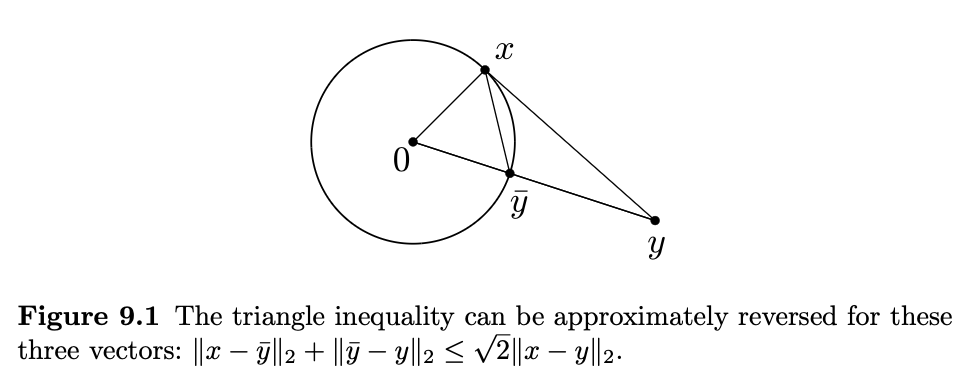
\includegraphics[width=0.8\textwidth]{Chapter 9/fig9-1.png}
\end{center}
Then by triangle inequality:
\[ \lVert Z_x - Z_y \rVert_{\psi_2} \leq \lVert Z_x - Z_{\bar{y}} \rVert_{\psi_2} 
+ \lVert Z_{\bar{y}} - Z_y \rVert_{\psi_2}. \]
Since both $x, \bar{y}$ are unit vectors, the result of Step 3 handles the first term:
\[ \lVert Z_x - Z_{\bar{y}} \rVert_{\psi_2} \leq CK^2 \lVert x - \bar{y} \rVert_{2}. \]
To handle the second term, note that $\bar{y}$ and $y$ are colinear vectors. So by homogeneity, 
\[ \lVert Z_{\bar{y}} - Z_y \rVert_{\psi_2} = \lVert \bar{y} - y \rVert_{2} \cdot \lVert Z_{\bar{y}} 
\rVert_{\psi_2}. \]
Now, since $\bar{y}$ is a unit vector, the result of Step 1 gives $\lVert Z_{\bar{y}} \rVert_{\psi_2} 
\leq CK^2$. Conbining the two terms, we conclude that 
\[ \lVert Z_x - Z_y \rVert_{\psi_2} \leq CK^2 (\lVert x - \bar{y} \rVert_{2} + \lVert \bar{y} - y \rVert_{2}). \]
At first this looks bad - we wnat to bound right hand side by $\lVert x - y \rVert_{2}$, but the triangle 
inequality goes the other way! Luckily, in our case (via the projection of $y$), the triangle inequality can be 
approximately reversed (Exercise 9.1):
\[ \lVert x - \bar{y} \rVert_{2} + \lVert \bar{y} - y \rVert_{2} \leq \sqrt{2}\lVert x - y \rVert_{2}. \]
Plugging this into the bound above, we get the desired bound:
\[ \lVert Z_x - Z_y \rVert_{\psi_2} \leq \sqrt{2}CK^2 \lVert x - y \rVert_{2}, \]
which proves the theorem.
\end{proof}

\begin{remark}[Matrix deviations from the mean]
\label{rmk:9.1.3}
A quick centering trick turns \cref{thm:9.1.1} into a deviation inequality around the mean 
$\mathbb{E}\left[ \lVert Ax \rVert_{2} \right]$ (Exercise 9.2).
\end{remark}

\begin{remark}[Matrix deviations: a high-probability bound]
\label{rmk:9.1.4}
We only stated \cref{thm:9.1.1} as an expectation bound, but we can upgrade it to a high-probability bound via 
the high-probability version of Talagrand's inequality (Exercise 8.37(b)). For any $u \geq 0$, the event 
\[ \sup_{x \in T} \left| \lVert Ax \rVert_{2} - \sqrt{m}\lVert x \rVert_{2} \right| 
\leq CK^2 [w(T) + u \cdot \mathrm{rad}(T)] \]
holds with probability at least $1 - 2 \exp{(-u^2)}$. Can you see why the above implies the expectation bound?
\end{remark}

\begin{remark}[Matrix deviations of squares]
\label{rmk:9.1.5}
If you are interested in deviations of the quadratic process $\lVert Ax \rVert_{2}^2$, we can also deduce this 
from \cref{thm:9.1.1} (Exercise 9.3):
\[ \mathbb{E}\left[ \sup_{x \in T} \left| \lVert Ax \rVert_{2}^2 - m \lVert x \rVert_{2}^2 \right| \right] 
\leq CK^4 \gamma(T)^2 + CK^2 \sqrt{m} \mathrm{rad}(T) \gamma(T). \]
\end{remark}



% ----------9.2----------
\subsection{Random Matrices, Covariance Estimation, and Johnson-Lindenstrauss}
The matrix deviation inequality has lots of useful consequences. We'll go over a few of them in this chapter!


\subsubsection{Singular Values of Random Matrices}
Applying the matrix deviation inequality for the unit Euclidean sphere $T = S^{n - 1}$ gives us the singular 
value bounds from Chapter 4.

Here is the quick check: since for the sphere we have 
\[ \mathrm{rad}(T) = 1 \text{ and } w(T) \leq \sqrt{n}, \]
the matrix deviation inequality shows that the event 
\[ \sqrt{m} - CK^2 (\sqrt{n} + u) \leq \lVert Ax \rVert_{2} \leq \sqrt{m} + CK^2 (\sqrt{n} + u) \text{ for 
all } x \in S^{n - 1} \]
holds with probability at least $1 - 2 \exp{(-u^2)}$. Then taking the min/max gives 
\[ \sqrt{m} - CK^2 (\sqrt{n} + u) \leq \sigma_n(A) \leq \sigma_1(A) \leq \sqrt{m} + CK^2 (\sqrt{n} + u) 
\text{ for all } x \in S^{n - 1}, \]
giving \cref{thm:4.6.1} in a different way.


\subsubsection{Random Projections of Sets}
From the matrix deviation inequality, we also get a sharper bound on the random projection bound in Section 7.6:

\begin{proposition}[Sizes of random projections of sets]
\label{prop:9.2.1}
Let $T \subset \mathbb{R}^n$ be a bounded set, and let $A$ be an $m \times n$ matrix with independent, isotropic 
and subgaussian rows $A_i$. Then the scaled matrix $P = \frac{1}{\sqrt{n}}A$ (a subgaussian projection) satisfies
\[ \mathbb{E}\left[ \mathrm{diam}(PT) \right] \leq \sqrt{\frac{m}{n}}\mathrm{diam}(T) + CK^2 w_s(T). \]
Here $K = \max_{i}\lVert A_i \rVert_{\psi_2}$ and $w_s(T)$ is the spherical width of $T$.
\end{proposition}


\begin{proof}
\cref{thm:9.1.1} implies via triangle inequality:
\[ \mathbb{E}\left[ \sup_{x \in T}\lVert Ax \rVert_{2} \right] \leq \sqrt{m}\sup_{x \in T}\lVert x \rVert_{2} 
+ CK^2 \gamma(T), \]
which we can rewrite in terms of the radii of $AT$ and $T$:
\[ \mathbb{E}\left[ \mathrm{rad}(AT) \right] \leq \sqrt{m}\mathrm{rad}(T) + CK^2 \gamma(T). \]
Applying this bound for the difference set $T - T$ instead of $T$ to get 
\[ \mathbb{E}\left[ \mathrm{diam}(AT) \right] \leq \sqrt{m}\mathrm{diam}(T) + 2CK^2w(T), \]
where we used \cref{lem:7.5.11} (a) to pass from Gaussian complexity to Gaussian width. Divide both sides by 
$\sqrt{n}$ completes the proof.
\end{proof}


\subsubsection{Covariance Estimation for Low-dimensional Distributions}
Let's visit the covariance estimation problem from Section 4.7. We want to estimate the population covariance 
via the sample covariance matrix $\Sigma_m = \sum_{i = 1}^{m}X_iX_i^T$.

In general, $O(n \log_{}{n})$ samples are enough (Section 5.6), but for subgaussian distributions, $m = O(n)$ 
is enough.

It gets even better for approximately low-dimensional distributions. If a distribution concentrates near a 
$r$-dimensional subspace, $m = O(r \log_{}{n})$ samples suffice (\cref{rmk:5.6.3}). Now we will show that for 
subgaussian distributions, $m = O(r)$ samples suffices:

\begin{theorem}[Covariance estimation for low-dimensional distributions]
\label{thm:9.2.2}
Let $X$ be a subgaussian random vector in $\mathbb{R}^n$. More spefically, assume that these exists $K \geq 1$ 
such that 
\[ \lVert \left\langle X, x \right\rangle \rVert_{\psi_2} \leq K \lVert \left\langle X, x 
\right\rangle \rVert_{L^2} \text{ for any } z \in \mathbb{R}^n. \]
Then, for every positive integer $m$, 
\[ \mathbb{E}\left[ \lVert \Sigma_m - \Sigma \rVert_{} \right] \leq CK^4 \left( 
\sqrt{\frac{r}{m}} + \frac{r}{m} \right) \lVert \Sigma \rVert_{}, \]
where $r = \mathrm{tr}(\Sigma)/\lVert \Sigma \rVert_{}$ is the effective rank of $\Sigma$.
\end{theorem}

\begin{proof}
We start as in \cref{thm:4.7.1} by bringing the distribution to the isotropic position: $X = \Sigma^{1/2}Z$ and 
$X_i = \Sigma^{1/2}Z_i$ where $Z$ and $Z_i$ are isotropic, and 
\begin{align*}
	\lVert \Sigma_m - \Sigma \rVert_{} 
	&= \lVert \Sigma^{1/2} E_m \Sigma^{1/2} \rVert_{} \quad (R_m = \frac{1}{m}\sum_{i = 1}^{m}Z_iZ_i^T - I_n) \\
	&= \max_{x \in S^{n-1}} |x^T \Sigma^{1/2} R_m \Sigma^{1/2} x| \quad \text{(\cref{rmk:4.1.12})} \\
	&= \max_{x \in T}|x^T R_m x| \quad (T := \Sigma^{1/2}S^{n-1}) \\
	&= \max_{x \in T} \left| \frac{1}{m}\sum_{i = 1}^{m}\left\langle Z_i, x \right\rangle^2 - 
	\lVert x \rVert_{2}^2 \right| \\
	&= \frac{1}{m}\max_{x \in T} \left| \lVert Ax \rVert_{2}^2 - m \lVert x \rVert_{2}^2 \right|,
\end{align*}
where $A$ is the $m \times n$ matrix with ros $Z_i$. As in the proof of \cref{thm:4.7.1}, $Z_i$ are isotropic, 
and satisfy $\lVert Z_i \rVert_{\psi_2} \lesssim 1$. This allows us to apply the matrix deviation inequality 
for $A$ (in the form given by Exercise 9.3), which gives
\[ \mathbb{E}\left[ \lVert \Sigma_m - \Sigma \rVert_{} \right] \lesssim 
\frac{1}{m}(\gamma(T)^2 + \sqrt{m}\mathrm{rad}(T)\gamma(T)). \]
The radius and Gaussian complexity of the ellipsoid $T = \Sigma^{1/2}S^{n-1}$ satisfy 
\[ \mathrm{rad}(T) = \lVert \Sigma \rVert_{}^{1/2} \text{ and } \gamma(T) \leq (\mathrm{tr}(\Sigma))^{1/2}. \]
Therefore, 
\[ \mathbb{E}\left[ \lVert \Sigma_m - \Sigma \rVert_{} \right] \lesssim 
\frac{1}{m} (\mathrm{tr}(\Sigma) + \sqrt{m \lVert \Sigma \rVert_{} \mathrm{tr}(\Sigma)}). \]
Substituting $\mathrm{tr}(\Sigma) = r \lVert \Sigma \rVert_{}$ and simplifying the bound completes the proof.
\end{proof}

\begin{remark}[Covariance estimation: a high-probability guarantee]
\label{rmk:9.2.4}
Just like the versions before (\cref{rmk:4.7.3} and \cref{rmk:5.6.5}), we can upgrade the expectation bound 
above to a high-probability one. For any $u \geq 0$ we have 
\[ \lVert \Sigma_m - \Sigma \rVert_{} \leq CK^4 \left( 
\sqrt{\frac{r + u}{m}} + \frac{r + u}{m} \right) \lVert \Sigma \rVert_{} \]
with probability at least $1 - 2e^{-u}$. 
\end{remark}

\begin{proof}
Exercise 9.9.
\end{proof}


\subsubsection{Johnson-Lindenstrauss Lemma for Infinite Sets}
The matrix deviation inequality quickly recovers the Johnson-Lindenstrauss lemma from Section 5.3 - and extends 
it to general, possibly infinite, sets.

To get a version of the JL lemma from matrix deviation, fix any $N$-point set $\mathcal{X} \in \mathbb{R}^n$ 
and consider the normalized differences: 
\[ T := \left\{ \frac{x - y}{\lVert x - y \rVert_{2}}: \ x, y \in \mathcal{X} \text{ distinct} \right\}. \]
The Gaussian complexity of $T$ satisfies 
\[ \gamma(T) \leq C \sqrt{\log_{}{N}}. \]
The matrix deviation inequality (\cref{thm:9.1.1}) shows that with high probability, 
\[ \sup_{x, y \in \mathcal{X}} \left| \frac{\lVert Ax - Ay \rVert_{2}}{\lVert x - y \rVert_{2}} - 
\sqrt{m} \right| \lesssim \sqrt{\log_{}{N}}. \]
Rearranging the terms, rewrite this as follows: the random matrix $Q := \frac{1}{\sqrt{m}}A$ is an approximate 
isometry on $\mathcal{X}$, i.e.
\[ (1 - \varepsilon)\lVert x - y \rVert_{2} \leq \lVert Qx - Qy \rVert_{2} \leq (1 + \varepsilon)\lVert x - y
\rVert_{2} \text{ for all } x, y \in \mathcal{X}, \]
for some $\varepsilon \asymp \sqrt{\log_{}{(N)} / m}$. Equivalently, if we fix $\varepsilon > 0$ and choose 
\[ m \gtrsim \varepsilon^{-2} \log_{}{N}, \]
then with high probability $Q$ is an $\varepsilon$-isometry on $\mathcal{X}$, which recovers a version of the 
classical JL lemma.

What we just not gave did not care if $\mathcal{X}$ is finite or not - all that matters is the Gaussian width. 
So we can extend JL to any set:

\begin{lemma}[Additive Johnson-Lindenstrauss lemma]
\label{lem:9.2.4}
Let $\mathcal{X} \subset \mathbb{R}^n$ be a bounded set, and let $A$ be an $m \times n$ matrix with independent, 
isotropic and subgaussian rows $A_i$. Then, with high probability (say 0.99), the scaled matrix $Q = 
\frac{1}{\sqrt{m}}A$ satisfies 
\[ |\lVert Qx - Qy \rVert_{2} - \lVert x - y \rVert_{2}| \leq \delta \text{ for all } x, y \in \mathcal{X} \]
where $\delta = CK^2w(\mathcal{X}) / \sqrt{m}$ and $K = \max_{i}\lVert A_i \rVert_{\psi_2}$.
\end{lemma}

\begin{proof}
Apply the matrix deviation inequality (\cref{thm:9.1.1}) for the set of differences $T = \mathcal{X}-
\mathcal{X}$. Then, with high probability, 
\[ \sup_{x, y \in \mathcal{X}} \left| \lVert Ax - Ay \rVert_{2} - \sqrt{m}\lVert x - y \rVert_{2} \right| 
\leq CK^2 \gamma(\mathcal{X}-\mathcal{X}) = 2CK^2 w(\mathcal{X}), \]
thanks to \cref{lem:7.5.11} (a). Divide both sides by $\sqrt{m}$ completes the proof.
\end{proof}

Unlike the classical JL lemma for finite sets (\cref{thm:5.3.1}), which gives a relative error, here we get an 
absolute error $\delta$. It is a small difference - but in general, a necessary one (Exercise 9.11).

\begin{remark}[Effective dimension]
\label{rmk:9.2.5}
To better understand the additive Johnson-Lindenstrauss lemma, let's restate it using the effective dimension of 
the data $d(\mathcal{X}) \asymp w(\mathcal{X})^2 / \mathrm{diam}(\mathcal{X})^2$. If we choose 
\[ m \gtrsim \varepsilon^{-2} d(T) \]
(ignoring the dependence on $K$ for simplicity), then we can make $\delta = \varepsilon \mathrm{diam}
(\mathcal{X})$, so $Q$ preserves distances up to a small fraction of diameter - in other words, it reduces the 
dimension of the data down to its effective dimension.
\end{remark}



% ----------9.3----------
\subsection{Random Sections: The \texorpdfstring{$M^*$}{} Bound and Escape Theorem}
Here is a surprising high-dimensional fact: if you slice a convex set $T \subset \mathbb{R}^n$ with a random 
subspace $E$ of codimension $m$, the slice $T \subset E$ is often tiny - even when $m \ll n$ and $E$ is near 
full-dimensional! Let's see how this follows from the matrix deviation inequality.


\subsubsection{The \texorpdfstring{$M^*$}{} Bound}
It is handy to model a random subspace $E$ as the kernel of an $m \times n$ random matrix: $E = \ker{A}$. We 
always have 
\[ \dim{(E)} \geq n - m, \]
and if $A$ has a continuous distribution, $\dim{(E)} \geq n - m$ almost surely.

A great example is a Gaussian matrix $A$ with i.i.d. $N(0, 1)$ entries - by rotation invariance, $E - \ker{(A)}$ 
is uniformly distributed in the Grassmannian:
\[ E \sim \mathrm{Unif}(G_{n, n - m}). \]

\begin{theorem}[$M^*$ bound]
\label{thm:9.3.1}
Let $T \subset \mathbb{R}^n$ be a bounded set, and $A$ be an $m \times n$ random matrix with independent, 
isotropic and subgaussian rows $A_i$. Then the random subspace $E = \ker{A}$ satisfies 
\[ \mathbb{E}\left[ \mathrm{diam}(T \cap E) \right] \leq \frac{CK^2 w(T)}{\sqrt{m}}, \]
where $K = \max_{i}\lVert A_i \rVert_{\psi_2}$.
\end{theorem}

\begin{proof}
Apply \cref{thm:9.1.1} for $T - T$:
\[ \mathbb{E}\left[ \sup_{x, y \in T} \left| \lVert Ax - Ay \rVert_{2} - \sqrt{m}\lVert x - y \rVert_{2} \right| 
\leq CK^2 \gamma(T - T) = 2CK^2 w(T), \right] \]
by \cref{lem:7.5.11} (a). Considering only the points $x, y$ in the kernel of $A$ makes $\lVert Ax - Ay 
\rVert_{2}$ disappear since $Ax = Ay = 0$. Divide both sides by $\sqrt{m}$ to get 
\[ \mathbb{E}\left[ \sup_{x, y \in T \cap \ker{A}} \lVert x - y \rVert_{2} \right] 
\leq \frac{CK^2 w(T)}{\sqrt{m}}, \]
which is exactly what we claimed.
\end{proof}

\begin{example}[The cross-polytope]
Let's apply the $M^*$ bound to the cross-polytope $B_1^n$ - the unit ball of the $\ell^1$ norm. Since its 
Gaussian width id roughly $\sqrt{\log_{}{n}}$ by \cref{ex:7.5.8}, we get 
\[ \mathbb{E}\left[ \mathrm{diam}(B_1^n \cap E) \right] \lesssim \sqrt{\frac{\log_{}{n}}{m}}. \]
For example, if $m = 0.01n$, then 
\[ \mathbb{E}\left[ \mathrm{diam}(T \cap E) \right] \lesssim \sqrt{\frac{\log_{}{n}}{n}}. \]
So, a random $0.99n$-dimensional slice of a cross-polytope is tiny!
\end{example}

How can this be? This relates to what we discussed in \cref{rmk:7.5.10}. The ``bulk" of $B_1^n$ is concentrated 
near the inscribed ball of radius $1/\sqrt{n}$, while the rest stretches out into long, thin ``spikes" along 
the coordinate axes. A random subspace $E$ probably misses those spikes and cuts through the bulk (Figure 9.2a). 
Therefore the slice ends up with diameter about $O(1/\sqrt{n})$, maybe with a log factor as shown above. This 
intuition can be extended to general convex sets as well.

\begin{center}
	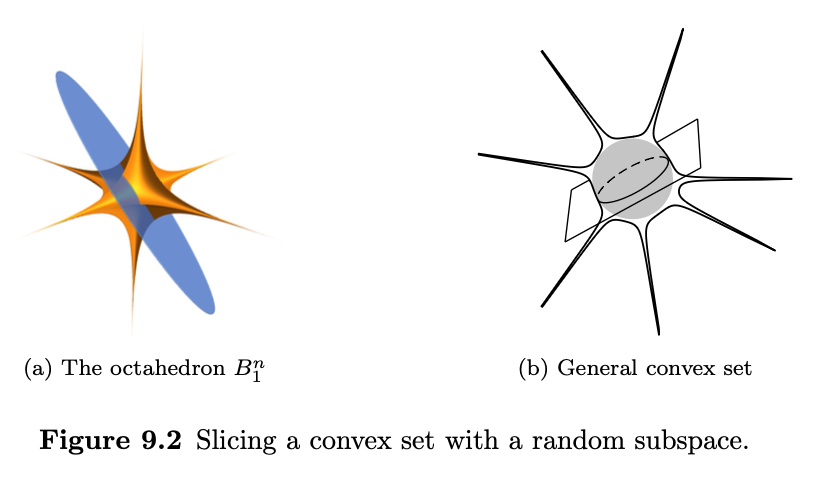
\includegraphics[width=0.8\textwidth]{Chapter 9/fig9-2.png}
\end{center}

\begin{remark}[Effective dimension]
\label{rmk:9.3.3}
To get more intuition, write the $M^*$ bound using the effective dimension (\cref{def:7.5.12}). The $M^*$ bound 
shows that slicing shrinks the dimaeter:
\[ \mathbb{E}\left[ \mathrm{diam}(T \cap E) \right] \leq 0.01 \cdot \mathrm{diam}(T) \]
as long as $m \gtrsim d(T)$. Since $\dim{(E)} = n - m$, this condition is equivalent to 
\[ \dim{(E)} + cd(T) \leq n. \]
That lines up with the linear algebra intuition: If $T$ is a cnetered Euclidean ball in some subspace 
$F \subset \mathbb{R}^n$, slicing can shrink the diameter of $T$ only when $\dim{E} + \dim{F} \leq n$.
\end{remark}


\subsubsection{The Escape Theorem}
When does a random subspace $E$ miss a given set $T$ entirely with high probability? Not if $T$ contains the 
origin - but if $T$ lies on the unit sphere (Figure 9.3), then it does as long as the codimension of $E$ is not 
too small: 

\begin{center}
	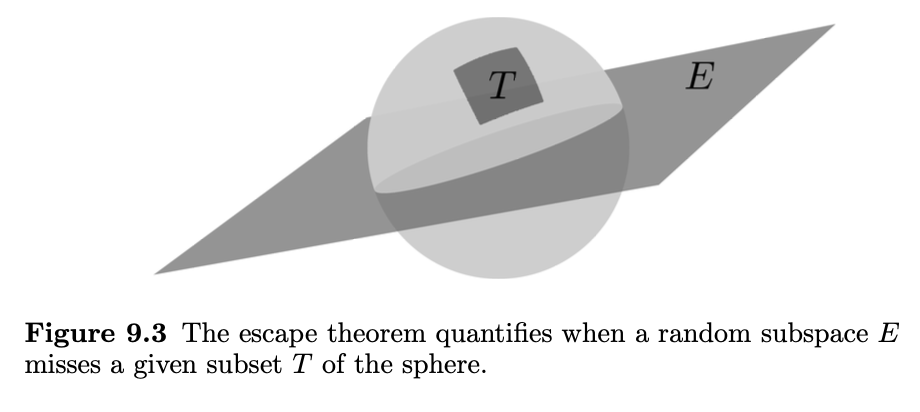
\includegraphics[width=0.8\textwidth]{Chapter 9/fig9-3.png}
\end{center}

\begin{theorem}[Escape theorem]
\label{thm:9.3.4}
Let $T \subset S^{n - 1}$ be any set, and let $A$ be an $m \times n$ matrix with independent, isotropic and 
subgaussian rows $A_i$. If 
\[ m \geq CK^4 w(T)^2, \]
then the random subspace $E = \ker{A}$ satisfies 
\[ T \cap E = \emptyset \]
with probability ar least $1 - 2 \exp{(-cm/K^4)}$. Here $K = \max_{i}\lVert A_i \rVert_{\psi_2}$.
\end{theorem}

\begin{proof}
Let us use the high-probability version of the matrix deviation inequality (\cref{rmk:9.1.4}): With probability 
at least $1 - 2 \exp{(-u^2)}$, 
\[ \sup_{x \in T}\left| \lVert Ax \rVert_{2} - \sqrt{m} \right| \leq C_1K^2(w(T) + u). \]
Suppose the above occurs. If $T \cap E \neq \emptyset$, then for any $x \in T \cap E$ we have $Ax = 0$, so 
\[ \sqrt{m} \leq C_1 K^2 (w(T) + u). \]
Set $u = \sqrt{m}/(2C_1K^2)$ and simplify this bound to get 
\[ \sqrt{m} \leq 2 C_1 K^2 w(T), \]
which contradicts the assumption if $C$ is large enough.Therefore, with that choice of $u$, the event implies 
$T \cap E = \emptyset$. Done!
\end{proof}


% ----------9.4----------
\subsection{Application: High-dimensional Linear Models}
Let's apply our tools on a classic data science problem: learning a linear model in high dimensions. Let 
\[ y_i = \left\langle A_i, x \right\rangle + w_i, \ i = 1, \dots, m. \]
Her $A_i \in \mathbb{R}^n$ are known, and $w_i$ are unknown numbers representing noise (Figure 9.4). In matrix form, we get 
\[ y = Ax + w. \]
The goal is to recover $x$ from $y$ and $A$ as accurately as possible. 

\begin{center}
	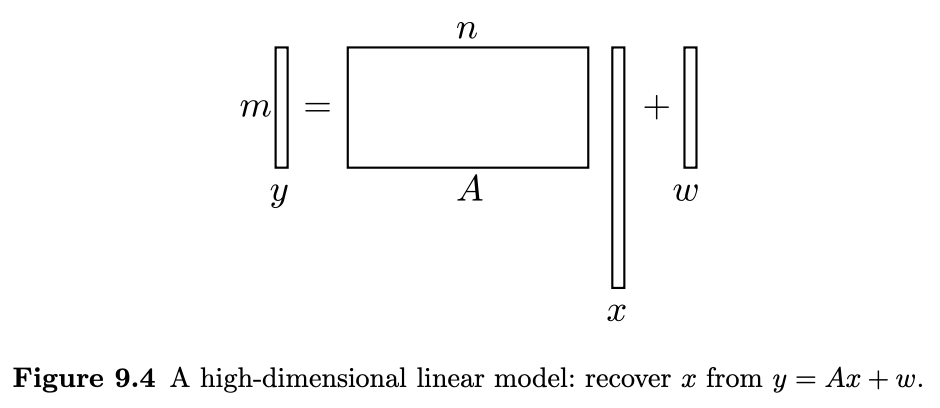
\includegraphics[width=0.8\textwidth]{Chapter 9/fig9-4.png}
\end{center}

We assume the rows $A_i$ of $A$ are random and independent - this is reasonable in many statistical settings 
(think about i.i.d. observations), and perfect for applying tools from high-dimensional probability.

\begin{example}[Audio sampling]
\label{ex:9.4.1}
In signal processing, $x$ could be a digitized audio signal, and $y$ the result of sampling it at $m$ random 
time points (Figure 9.5).

\begin{center}
    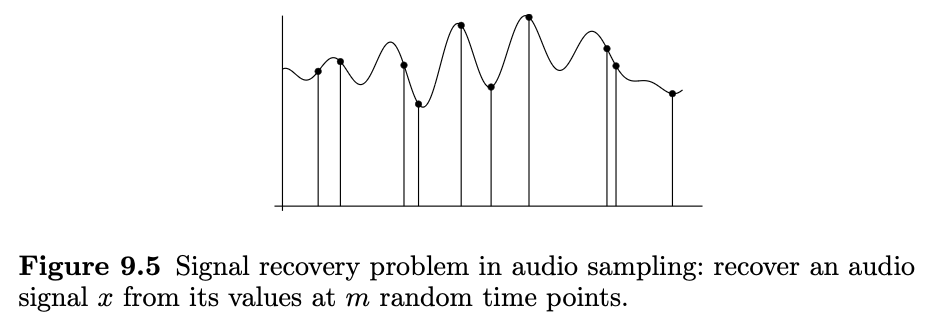
\includegraphics[width=0.8\textwidth]{Chapter 9/fig9-5.png}
\end{center}
\end{example}

\begin{example}[Linear regression]
\label{ex:9.4.2}
A core porblem in statistics is linear regression, where we want to learn a linear relationship between $n$ 
predictor variables and a response variable from $m$ samples. It is written as 
\[ Y = X \theta + w \]
where $X$ is an $m \times n$ matrix of predictors, $Y \in \mathbb{R}^m$ is the vector of responses, $\theta \in 
\mathbb{R}^n$ is the parameter vector that we are trying to learn.
\end{example}

\begin{remark}[The high-dimensional regime]
\label{rmk:9.4.3}
In modern problems, we often have less data than parameters: 
\[ m \ll n, \]
For example, in a genetic study, there might be $\sim$100 patients, but $\sim$10000 genes. In this 
high-dimensional setting, even solving $Ax  = y$ becomes impossible, as there are too many possible solutions 
as they live in a large subspace of dimension at least $m - n$.

Not all hope is lost. If we have some prior information about the structure of $x$, which we can write this as 
\[ x \in T \]
for some known set $T \subset \mathbb{R}^n$, then we might be able to recover $x$. For example, if $x$ is 
sparse, we can pick $T$ to be the set of all sparse vectors.
\end{remark}


\subsubsection{Constrained Recovery}
Let's solve the noiseless case first:
\[ y = Ax, \ x \in T. \]
How do we solve this dimensional constrained linear problem?

A simple idea is just to pick any vector $x' \in T$ that matches the observations:
\[ \text{find } x': \ y = Ax', \ x \in T. \]
If $T$ is convex, this is a convex program, and many algorithms exist to numerically solve it. Let's check 
how accurate this solution is.

\begin{theorem}[Constrained recovery]
\label{thm:9.4.4}
Suppose the rows $A_i$ of $A$ are independent, isotropic and subgaussian random vectors. Then any solution 
$\Hat{x}$ of the convex linear program satisfies 
\[ \mathbb{E}\left[ \lVert \Hat{x} - x \rVert_{2} \right] \leq \frac{CK^2 w(T)}{\sqrt{m}}, \]
where $K = \max_{i}\lVert A_i \rVert_{\psi_2}$.
\end{theorem}

\begin{proof}
Since $x, \Hat{x} \in T$ and $Ax = A \Hat{x} = y$, we have 
\[ x, \Hat{x} \in T \cap E_x, \text{ where } E_x = x + \ker{A} \]
See Figure 9.6 for an illustration.

\begin{center}
    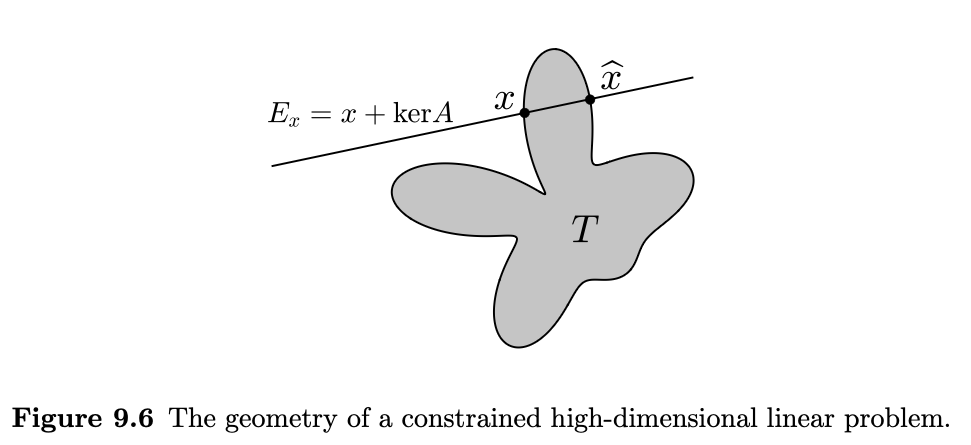
\includegraphics[width=0.8\textwidth]{Chapter 9/fig9-6.png}
\end{center}
Then the $M^*$ bound (in the form of Exercise 9.12) gives 
\[ \mathbb{E}\left[ \lVert \Hat{x} - x \rVert_{2} \right] 
\leq \mathbb{E}\left[ \mathrm{diam}(T \cap E_x) \right] \leq \frac{CK^2 w(T)}{\sqrt{m}}. \]
\end{proof}

\begin{remark}[Effective dimension]
\label{rmk:9.4.5}
To get some intuition, rewrite the accuracy guarantee in \cref{thm:9.4.4} using the effective dimension 
(\cref{def:7.5.12}). We get a nontrivial error bound 
\[ \mathbb{E}\left[ \lVert \Hat{x} - x \rVert_{2} \right] \leq 0.01 \mathrm{diam}(T) \]
as long as the number of observations satisfies (suppressing $K$ again)
\[ m \gtrsim d(T). \]
Since $d(T)$ can be much smaller than the ambient dimension $n$, recovery is often possible even in the 
high-dimensional regime.
\end{remark}

\begin{remark}[Convex relaxation]
\label{rmk:9.4.6}
If $T$ is not convex, we can just use its convex hull $\mathrm{conv}(T)$. The recovery guarantees from 
\cref{thm:9.4.4} do not change, as $w(\mathrm{conv}(T)) = w(T)$ by \cref{prop:7.5.2} (c).
\end{remark}

\begin{remark}[Unconstrained optimization]
\label{rmk:9.4.7}
Forcing strict rules on the solution like $y = Ax'$ and $x' \in T$ can be too rigid - noise or a bad choice for 
$T$ might mean no solution exists. Instead, we could aim to penalize how much they are broken by solving the 
unconstrained convex problem 
\[ \min_{}\lVert y - Ax \rVert_{2}^2 + \lambda \lVert x \rVert_{T}, \ x \in \mathbb{R}^n, \]
where $\lVert \cdot \rVert_{T}$ is any norm you like, and $\lambda > 0$ is a parameter we can adjust to see 
which summand we want to prioritize more.
\end{remark}


We also have the following guarantee from Exercise 9.20: if $A$ is an $m \times n$ random matrix, and $\lambda$ 
is chosen well, then the solution $\Hat{x}$ satisfies 
\[ \mathbb{E}\left[ \lVert \Hat{x} - x \rVert_{2} \right] \lesssim 
\frac{w(T)\lVert x \rVert_{T} + \lVert w \rVert_{2}}{\sqrt{m}}, \]
where $T$ is the unit ball of $\lVert \cdot \rVert_{T}$. 

In short, if $x$ is well structured and the noise $w$ is small, then you can recover $x$ accurately from 
$m \asymp d(T)$ observations, where $d(T)$ is the effective dimension of $T$.


\subsubsection{Example: Sparse Recovery}
Sometimes we believe that $x$ is \textit{sparse} - most of its entries are zero or nearly zero. We can 
quantify the sparsity of $x \in \mathbb{R}^n$ by the number of nonzero entries:
\[ \lVert x \rVert_{0} = |\mathrm{supp}(x)| = |\{ i: \ x_i \neq 0 \}|, \]
and we say that $x$ is sparse if $\lVert x \rVert_{0} \leq s$. The ``$\ell^0$ norm" is not really a norm, but 
is a limit of $\ell^p$ norms as $p \to 0$ (Exercise 9.23).

A quick dimension count shows that we can recover $x$ from $y = Ax$ if $A$ is in a general position and we have 
enough observations: $m \geq 2 \lVert x \rVert_{0}$ (Exercise 9.22). Sounds great, as we can recover a sparse 
vector from only a few observations. The catch? It's computationally hard unless we already know the support of 
$x$. Without that, the best way is to brute force - $\binom{n}{s} \geq 2^s$ subsets to check!

To solve this, we can pick the prior using the $\ell^1$ norm, the closest $\ell^p$ that is actually a norm 
(Exercise 9.23). Since $s$-sparse vectors with $\lVert x \rVert_{2} \leq 1$ satisfy $\lVert x \rVert_{2} \leq 
\sqrt{s}$, it makes sense to pick the convex set 
\[ T := \sqrt{s}B_1^n \]
as our prior. The recovery program becomes 
\[ \text{find } x: \ y = Ax, \ \lVert x \rVert_{1} \leq \sqrt{s}. \]

\begin{corollary}[Sparse recovery]
\label{cor:9.4.8}
Suppose the rows $A_i$ of $A$ are independent, isotropic and subgaussian random vectors. Assume an unknown 
$s$-sparse vector $x \in \mathbb{R}^n$ satisfies $\lVert x \rVert_{2} \leq 1$. Then any solution $\Hat{x}$ to 
the program above satisfies 
\[ \mathbb{E}\left[ \lVert \Hat{x} - x \rVert_{2} \right] \leq CK^2 \sqrt{\frac{s \log_{}{n}}{m}}, \]
where $K = \max_{i}\lVert A_i \rVert_{\psi_2}$.
\end{corollary}

\begin{proof}
Set $T = \sqrt{s}B_1^n$. Then the result follows from \cref{thm:9.4.4} and the bound on the Gaussian width 
of the $\ell^1$ ball: 
\[ w(T) = \sqrt{s}w(B_1^n) \leq C \sqrt{s \log_{}{n}}. \]
\end{proof}

\begin{remark}[Observations scale almost linearly with sparsity]
\label{rmk:9.4.9}
\cref{cor:9.4.8} gives a small error as long as
\[ m \gtrsim s \log_{}{n} \]
(if the hidden constant is appropriately large). That's great news - we can efficiently recover a sparse vector 
from way fewer observations $m$ than the full dimension $n$.
\end{remark}

\begin{remark}[A logarithmic improvement]
\label{rmk:9.4.10}
The set $S_{n, s}$ of unit $s$-sparse vectors in $\mathbb{R}^n$ can be convexified a bit tighter. Instead of 
using the $\ell^1$ ball, use the \textit{truncated} $\ell^1$ ball 
\[ T_{n,s} = \sqrt{s}B_1^n \cap B_2^n. \]
This relaxation is pretty tight - Exercise 9.25 gives 
\[ \mathrm{conv}(S_{n,s}) \subset T_{n,s} \subset 2\mathrm{conv}(S_{n,s}).  \]
This tightening gives a logarithmic improvement on the bound in \cref{cor:9.4.8}, showing that 
\[ m \gtrsim s \log_{}{(en/s)} \]
observations suffice for sparse recovery (Exercise 9.21).
\end{remark}


\subsubsection{Example: Low-rank Recovery}
Here is one more example of a high-dimensional linear problem: recover a $d \times d$ matrix $X$ (instead of 
a vector) from $m$ linear observations:
\[ y_i = \left\langle A_i, X \right\rangle, \ i = 1, \dots, m, \]
where $A_i$ are known, independent random matrices, adn the inner product is 
\[ \left\langle A, B \right\rangle = \mathrm{tr}(A^T B). \]

Normally, we would need $d^2$ observations - one per entry. To get away with fewer, we need some structure in 
$X$. A common one is low rank. Just like sparsity counts nonzero entries, rank counts nonzero singular values.

In section 9.4.2, we took a relaxation by replacing the $\ell^0$ norm with the $\ell^1$ norm. Here we'll use 
a convex relaxation by replacing the $\ell^0$ norm for the singular values with the $\ell^1$ norm, which 
is also known as the \textit{nuclear norm}:
\[ \lVert X \rVert_{*} := \sum_{i = 1}^{d} \sigma_i(X). \]

Since every vector $x$ with at most $s$ nonzero entries and $\lVert x \rVert_{2} \leq 1$ satisfies 
$\lVert x \rVert_{} \leq \sqrt{s}$, every matrix with rank at most $r$ and $\lVert X \rVert_{F} = 1$ satisfies 
\[ \lVert X \rVert_{*} \leq \sqrt{r}. \]
Therefore, it makes sense to consider $T = \sqrt{r}B_*$ as our prior, where 
\[ B_* = \{ X \in \mathbb{R}^{d \times d}: \ \lVert X \rVert_{*} \leq 1 \}. \]
Then, the recovery program becomes 
\[ \text{find } X: \ y_i = \left\langle A_i, X \right\rangle \forall i; \ \lVert X \rVert_{*} \leq \sqrt{r}, \]
which is convex and computationally tractable. And \cref{thm:9.4.4} gives 

\begin{corollary}[Low-rank matrix recovery]
\label{cor:9.4.11}
Suppose $A_i$ are independent Gaussian random matrices with all i.i.d. $N(0, 1)$ entries. Assume an unknown 
$d \times d$ matrix $X$ has rank at most $r$ and $\lVert X \rVert_{F} \leq 1$. Then any solution $\Hat{X}$ of 
the program satisfies 
\[ \mathbb{E}\left[ \lVert \Hat{X} - X \rVert_{F} \right] \leq C \sqrt{\frac{rd}{m}}. \]
\end{corollary}

\begin{proof}
Using the duality between the nuclear and operator norms (Exercise 7.18a), we get that for a $d \times d$ 
Gaussian matrix $G$ with i.i.d. $N(0, 1)$ entries:
\[ w(B_*) = \mathbb{E}\left[ \sup_{\lVert X \rVert_{*} \leq 1} \left\langle G, X \right\rangle \right] 
= \mathbb{E}\left[ \lVert G \rVert_{} \right] \leq 2 \sqrt{d} \]
by \cref{thm:7.3.1}. Now just apply \cref{thm:9.4.4} with $T = \sqrt{r}B_*$. 
\end{proof}

\begin{remark}[Recovering a low-rank matrix from few observations]
\label{rmk:9.4.12}
\cref{cor:9.4.8} gives a small error as long as
\[ m \gtrsim rd, \]
allowing us to recover a low-rank matrix from war fewer observations $m$ then the entirety $d^2$. This is 
similar to the matrix completion problem in Section 6.5, where we can recover a low-rank matrix from about 
$m \asymp rd \log_{}{d}$ randomly chosen entries.
\end{remark}



% ----------9.5----------
\subsection{Application: Exact Sparse Recovery}
In the noiseless case, we can do even better - we can recover a sparse vector $x$ from $y = Ax$ \textit{exactly} 
(and algorithmically effective)! We will look at two ways to get this surprising result:
\begin{enumerate}
	\item Use the escape theorem (\cref{thm:9.3.4}).
	\item Using the restricted isometry property - then show random matrices satisfy it with high probability.
\end{enumerate}


\subsubsection{Exact Recovery Based on the Escape Theorem}
Let's look at Figure 9.7 below for some intuition.

\begin{center}
	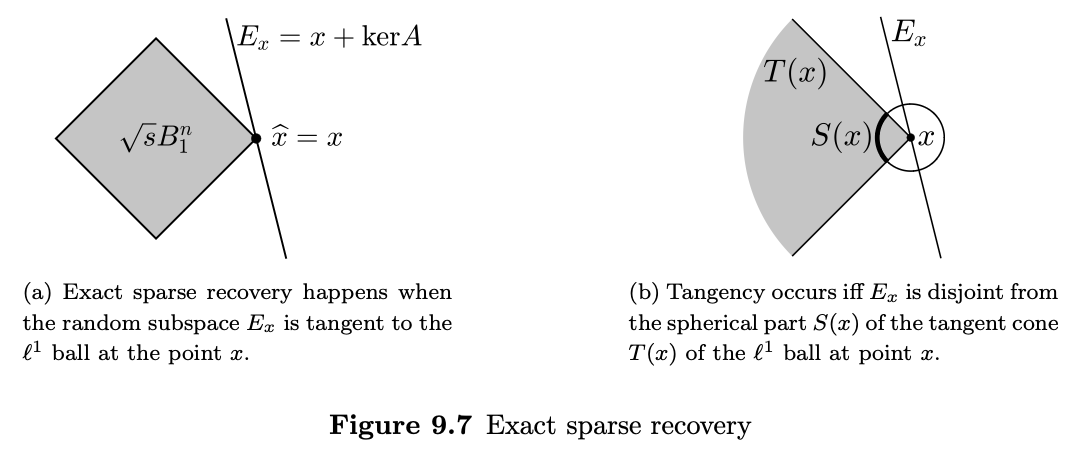
\includegraphics[width=0.8\textwidth]{Chapter 9/fig9-7.png}
\end{center}

Suppose we are trying to recover an unknown $s$-sparse unit vector $x$ from $y=Ax$ by solving the convex program 
in Section 9.4.2. A solution $\Hat{x}$ lies in the intersection of the prior set $T = \sqrt{s}B_1^n$ and the 
affine subspace $E_x = x + \ker{A}$.

$T$ is a cross-polytope, and $x$ sits on one of its $(s-1)$-dimensional edges (Figure 9.7a). With some 
probability, the random subspace $E_x$ is tangent to the polytope at $x$. If so, $x$ is the only point where 
$T$ and $E_x$ intersect, hence the solution $\Hat{x}$ must be exact:
\[ \Hat{x} = x. \]
To justify this argument, we just need to show that a random subspace $E_x$ is tangent to the $\ell^1$ ball 
with high probability. That's where the escape theorem (\cref{thm:9.3.4}) comes in. Zoom in near $x$
(Figure 9.7b): $E_x$ is tangent if and only if the \textit{tangent cone} $T(x)$ (all rays coming from x into 
the $\ell^1$ ball) intersects $E_x$ only at $x$. This happens if the \textit{spherical part} $S(x)$ of the 
cone (the intersection of $T(x)$ with a small sphere centered at $x$) is disjoint from $E_x$ – and that is 
exactly what the escape theorem can guarantee!

Let's formalize this. We want to recover $x$ from 
\[ y = Ax \]
by solving the optimization problem 
\[ \min_{}\lVert x \rVert_{1} \text{ subject to } y = Ax. \]

\begin{theorem}[Exact sparse recovery]
\label{thm:9.5.1} A $m \times n$ matrix $A$ with independent, isotropic, subgaussian rows $A_i$ satisfies the 
following with probability at least $1 - 2 \exp{(-cm/K^4)}$, where $K = \max_{i}\lVert A_i \rVert_{\psi_2}$:

If the number of observations satisfies 
\[ m \geq CK^4 s \log_{}{n}, \]
then for any $s$-sparse vector $x \in \mathbb{R}^n$, a solution $\Hat{x}$ of the convex program is exact:
\[ \Hat{x} = x. \]
\end{theorem}

To prove this, we want to show that the recovery error is 0:
\[ h := \Hat{x} - x = 0. \]
First, let's show a weaker claim: $h$ has more mass on the spport of $X$ than off it.

\begin{lemma}[The error is heavier on $x$'s support]
\label{lem:9.5.2}
Set $S := \mathrm{supp}(x)$, and let $h_S \in \mathbb{R}^S$ denote the restriction of $h$ onto $S$ (and 
similartly for $S^c$). Then 
\[ h_{S^c} \leq \lVert h_S \rVert_{1}. \]
\end{lemma}

\begin{proof}
Since $\Hat{x}$ is the minimizer in the program, we have 
\[ \lVert \Hat{x} \rVert_{1} \leq \lVert x \rVert_{1}. \]
But there is also a lower bound
\begin{align*}
	\lVert \Hat{x} \rVert_{1} 
	&= \lVert x + h \rVert_{1} \\
	&= \lVert x_S + h_S \rVert_{1} + \lVert x_{S^c} + h_{S^c} \rVert_{1} \\
	&\geq \lVert x \rVert_{1} - \lVert h_S \rVert_{1} + \lVert h_{S^c} \rVert_{1},
\end{align*}
where the last line follows by triangle inequality and using $x_S = x$ and $x_{S^c} = 0$. Substituting this 
into the first equation completes the proof.
\end{proof}

\begin{lemma}[The error is approximately sparse]
\label{lem:9.5.3}
The error vector satisfies 
\[ \lVert h \rVert_{1} \leq 2 \sqrt{s}\lVert h \rVert_{2}. \]
\end{lemma}

\begin{proof}
Using \cref{lem:9.5.2} and then the Cauchy-Schwartz inequality, we get 
\begin{align*}
	\lVert h \rVert_{1} 
	&= \lVert h_S \rVert_{1} + \lVert h_{S^\subset1} \rVert_{1} \\
	&\leq 2 \lVert h_S \rVert_{1} \\
	&\leq 2 \sqrt{s}\lVert h_S \rVert_{2} \\
	&\leq 2 \sqrt{s}\lVert h \rVert_{2}.
\end{align*}
\end{proof}

Now let's return to the proof for exact sparse recovery.
\begin{proof}[Proof of \cref{thm:9.5.1}]
Assume $h = \Hat{x} - x \neq 0$. \cref{lem:9.5.3} gives 
\[ \frac{h}{\lVert h \rVert_{2}} \in T_s := \{ z \in S^{n-1}: \ \lVert z \rVert_{1} \leq 2 \sqrt{s} \}. \]
Since also $Ah = A \Hat{x} - Ax = y - y = 0$, we have 
\[ \frac{h}{\lVert h \rVert_{2}} \in T_s \cap \ker{A}. \]
The escape theorem (\cref{thm:9.3.4}) shows that this intersection is empty with high probability as long as 
$m \geq C_1 K^4w(T_s)^2$. Now, since $T_s \subset 2 \sqrt{s}B_1^n$, we get
\[ w(T_s) \leq 2 \sqrt{s} w(B_1^n) \leq C_2 \sqrt{s \log_{}{n}}. \]
Thus, if $m \geq CK^4s \log_{}{n}$, the intersection $T_s \cap \ker{A}$ is empty with high probability, which 
means the inclusion in the first equation cannot hold. Therefore, our assumption that $h \neq 0$ is false 
with high probablity, and the proof is complete.
\end{proof}

\begin{remark}[Improving the logarithmic factor]
\label{rmk:9.5.4}
By slightly tightening the last equation from \cref{lem:9.5.3}, we can improve the number of sufficient 
observations in \cref{thm:9.5.1} to
\[ m \geq CK^4 s \log_{}{(en/s)}. \]
This follows from Exercise 9.26.
\end{remark}


\subsubsection{Restricted Isometries}
We'll now find a \textit{deterministic} condition that ensures a matrix $A$ works for sparse recovery, and 
prove that random matrices satisfy this condition. 

\begin{definition}[]
\label{def:9.5.5} 
An $m \times n$ matrix $A$ satisfies the \underline{restricted isometry property/RIP} with 
parameters $\alpha, \beta$, and $s$ if the inequality
\[ \alpha \leq \lVert v \rVert_{2} \leq \lVert Av \rVert_{2} \leq \beta \lVert v \rVert_{2} \]
holds for all vectors $v \in \mathbb{R}^n$ with at most $s$ nonzero entries.
\end{definition}

RIP just says that the singular values of all $m \times s$ submatrices $A_I$ of $A$ satisfy 
\[ \alpha \leq \sigma_s(A_I) \leq \sigma_1(A_i) \leq \beta. \]
And if $\alpha \approx \beta \approx 1$, then RIP tells us that all those submatrices are approximate 
isometries.

\begin{theorem}[RIP implies exact recovery]
\label{thm:9.5.6}
Suppose a $m \times n$ matrix $A$ satisfies TIP with some parameters $\alpha, \beta$, and $(1 + \lambda)s$, 
where $\lambda > (\beta/\alpha)^2$. Then every $s$-sparse vector $x \in \mathbb{R}^n$ can be exactly recovered 
from $y = Ax$ by solving the convex relaxation problem earlier.
\end{theorem}

\begin{proof}
As in the proof of \cref{thm:9.5.1}, we need to show that the error
\[ h = \Hat{x} - x \]
is zero. To do this, we decompose $h$ in a way ver similar to Exercise 9.25.

\textbf{Step 1: Decomposing the support.} Let $I_0$ be the support of $x$. Let $I_1$ index the $\lambda s$ 
largest entries of $h_{I_0^c}$ in magnitude, let $I_2$ index the next $\lambda s$ largest entries of 
$h_{I_0^c}$ in magnitude, and so on. Finally, set $I_{01} = I_0 \cup I_1$. Since 
\[ Ah = A \Hat{x} - Ax = y - y = 0, \]
the triangle inequality gives 
\[ 0 = \lVert Ah \rVert_{2} \geq \lVert A_{I_{01}}h_{I_{01}} \rVert_{2} - 
\lVert A_{I_{01}^c}h_{I_{01}^c} \rVert_{2}. \quad (*) \]
Next, let's look at the two terms on the right hand side.

\textbf{Step 2: Applying RIP.} Since $|I_{0,1}| \leq s + \lambda s$, RIP gives 
\[ \lVert A_{I_{01}} h_{I_{01}} \rVert_{2} \geq \alpha \lVert h_{I_{01}} \rVert_{2} \]
and the triangle inequality followed by RIP gives 
\[ \lVert A_{I_{01}^c}h_{I_{01}^c} \rVert_{2} \leq \sum_{i \geq 2}^{} \lVert A_{I_i}h_{I_i} \rVert_{2} 
\leq \beta \sum_{i \geq 2}^{} \lVert h_{I_i} \rVert_{2}. \]
Plugging into $(*)$ gives 
\[ \beta \sum_{i \geq 2}^{}\lVert h_{I_i} \rVert_{2} \geq \alpha \lVert h_{I_{0,1}} \rVert_{2}. \quad (**) \]

\textbf{Step 3: Summing up.} Nextm we bound the sum in the left like we did in Exercise 9.25. By definition 
of $I_i$, each entry of $h_{I_i}$ is bounded in magnitude by the average of the entries of $h_{I_{i - 1}}$, 
i.e. by $\frac{1}{\lambda_s}\lVert h_{I_{i-1}} \rVert_{1}$ for $i \geq 2$. Thus 
\[ \lVert h_{I_i} \rVert_{2} \leq \frac{1}{\sqrt{\lambda s}} \lVert h_{I_{i-1}} \rVert_{1}. \]
Summing up, we get 
\begin{align*}
	\sum_{i \geq 2}^{}\lVert h_{I_i} \rVert_{2} 
	&\leq \frac{1}{\sqrt{\lambda s}}\sum_{i \geq 1}^{}\lVert h_{I_i} \rVert_{1} \\
	&= \frac{1}{\sqrt{\lambda s}} \lVert h_{I_0^c} \rVert_{1} \\
	&\leq \frac{1}{\sqrt{\lambda s}} \lVert h_{I_0} \rVert_{1} \quad \text{(\cref{lem:9.5.2})} \\
	&\leq \frac{1}{\sqrt{\lambda}} \lVert h_{I_0} \rVert_{2} \\
	&\leq \frac{1}{\sqrt{\lambda}} \lVert h_{I_{0,1}} \rVert_{2}.
\end{align*}
Putting this into $(**)$, we get 
\[ \frac{\beta}{\sqrt{\lambda}}\lVert h_{I_{0,1}} \rVert_{2} \geq \alpha \lVert h_{I_{0,1}} \rVert_{2}. \]
But this implies that $h_{I_{0,1}} = 0$ since $\beta/\sqrt{\lambda} < \alpha$ by assumption. And since 
$I_{0,1}$ contains the largest entries of $h$, it must be that $h = 0$.
\end{proof}

While we do not know how to construct deterministic matries $A$ that satisfy RIP with good parameters, we can 
show that random matrices satisfy it with high probability:

\begin{theorem}[Random matrices satisfy RIP]
\label{thm:9.5.7}
Consider an $m \times n$ matrix $A$ with independent, isotropic, subgaussian rows $A_i$. Assume that 
\[ m \geq CK^4 s \log_{}{(en/s)} \]
where $K = \max_{i} \lVert A_i \rVert_{\psi_2}$. Then, with probability at least $1 - 2 \exp{(-cm/K^4)}$, 
the random matrix $A$ satisfies RIP with paremeters 
\[ \alpha = 0.9 \sqrt{m}, \beta = 1.1 \sqrt{m}, \text{ and } s. \]
\end{theorem}

\begin{proof}
We need to check that 
\[ \alpha \leq \sigma_s(A_I) \leq \sigma_1(A_i) \leq \beta. \]
for all $m \times s$ submatrices $A_I$. First, fix $I$. By \cref{thm:4.6.1}, we get 
\[ 0.9 \sqrt{m} \leq \sigma_s(A_I) \leq \sigma_1(A_I) \leq 1.1 \sqrt{m} \]
with probability at least $1 - 2 \exp{(-cm/K^4)}$ (set $t = \sqrt{2cm}/K$ and use the assumption on $m$, 
with constants $c$ and $C$ chosen appropriately).

Now take a union bound over all $\binom{n}{s}$ possible $s$-element subsets $I \subset \{ 1, \dots, n \}$. 
Then the above holds with probability at least 
\[ 1 - 2 \exp{(-cm/K^4)} \cdot \binom{n}{s} > 1 - 2 \exp{(-cm/K^4)}, \]
using the bound $\binom{n}{s} \leq \exp{(s \log_{}{(en/s)})}$ from Exercise 0.6 and the assumption on $m$. 
Hence the proof is complete.
\end{proof}

In fact, we just learned an alternative approach to exact recovery:

\begin{proof}[Second proof of \cref{thm:9.5.1}]
By \cref{thm:9.5.7}, $A$ satisfies RIP with $\alpha = 0.9 \sqrt{m}$, $\beta = 1.1 \sqrt{m}$, and $3s$. Thus, 
\cref{thm:9.5.6} for $\lambda = 2$ guarantees exact recovery. The proof is complete. We even get the 
logarithmic improvement from Exercise 9.5.4!
\end{proof}



% ----------9.6----------
\subsection{Deviations of Random Matrices for General Norms}
We can generalize the matrix deviation inequality (\cref{thm:9.1.1}) to work for any norm - not just the 
Euclidean one. Actually we don't even need the norm to be nonnegative - just homogeneity and triangle inequality 
is enough.

\begin{definition}[]
\label{def:9.6.1}
A real-valued function $f$ on a linear vector space $V$ is called:
\begin{itemize}
	\item \underline{Positive-homogeneous} if $f(\alpha x) = \alpha f(x)$ for all $\alpha \geq 0$ and $x \in V$;
	\item \underline{Subadditive} if $f(x + y) \leq f(x) + f(y)$ for all $x, y \in V$.
\end{itemize}
\end{definition}

\begin{example}[]
\label{ex:9.6.2}
These functions are positive-homogeneous and subadditive:
\begin{enumerate}
	\item Any norm;
	\item Any real-valued linear function (i.e. any \textit{linear functional});
	\item In particular, the function $f(x) = x^T y$ for any fixed vector $y \in \mathbb{R}^m$;
	\item the \textit{support function} of any bounded set $S \subset \mathbb{R}^n$, defined by 
	\[ f(x) := \sup_{y \in S}\left\langle x, y \right\rangle, \ x \in \mathbb{R}^m. \]
\end{enumerate}
\end{example}

We can make \cref{thm:9.1.1} work for all norms (even positive-homogeneous, subadditive functions), but with a 
tradeoff - it applies only to Gaussian matrices:

\begin{theorem}[General matrix deviation inequality]
\label{thm:9.6.3}
Let $A$ be an $m \times n$ random matrix with i.i.d. $N(0, 1)$ entries. Let $f: \mathbb{R}^m \to \mathbb{R}$ be 
a bounded, positive-homogeneous and subadditive function, and let $b \in \mathbb{R}$ such that 
\[ f(x) \leq b \lVert x \rVert_{2} \text{ for all } x \in \mathbb{R}^n. \]
Then for any subset $T \subset \mathbb{R}^n$, 
\[ \mathbb{E}\left[ \sup_{x \in T} \left| f(Ax) - \mathbb{E}\left[ f(Ax) \right] \right| \right] 
\leq Cb \gamma(T), \]
where $\gamma(T)$ is the Gaussian complexity.
\end{theorem}

With the same logic as in the proof for \cref{thm:9.1.1}, \cref{thm:9.6.3} would immediately follow from 
Talagrand's comparison inequality once we show that the random process
\[ Z_x := f(Ax) - \mathbb{E}\left[ f(Ax) \right] \]
has subgaussian increments. Let's do this :)

\begin{theorem}[Subgaussian increments]
\label{thm:9.6.4}
Let $A$ be an $m \times n$ Gaussian random matrix with i.i.d. $N(0, 1)$ entries, and let $f: \mathbb{R}^m \to 
\mathbb{R}$ be a positive homogeneous and subadditive function satisfying 
\[ f(x) \leq b \lVert x \rVert_{2} \text{ for all } x \in \mathbb{R}^n. \]
Then the random process 
\[ Z_x := f(Ax) - \mathbb{E}\left[ f(Ax) \right] \]
has subgaussian increments:
\[ \lVert Z_x - Z_y \rVert_{\psi_2} \leq Cb \lVert x - y \rVert_{2} \text{ for all } x, y \in \mathbb{R}^n. \]
\end{theorem}

\begin{proof}
Without loss of generality, we may assume that $b = 1$. Just like in the proof of \cref{thm:9.1.2}, first assume 
that 
\[ \lVert x \rVert_{2} = \lVert y \rVert_{2} = 1. \]
In this case, the inequality in the theorem becomes 
\[ \lVert f(Ax) - f(Ay) \rVert_{\psi_2} \leq C \lVert x - y \rVert_{2}. \]

\textbf{Step 1: Creating independence.} Consider the vectors 
\[ u := \frac{x + y}{2}, \ v := \frac{x - y}{2}. \]
Then $x = u + v$ and $y = u - v$, and thus 
\[ Ax = Au + Av, \ Ay = Au - Av \quad (\text{See Figure 9.8 below}) \]
\begin{center}
	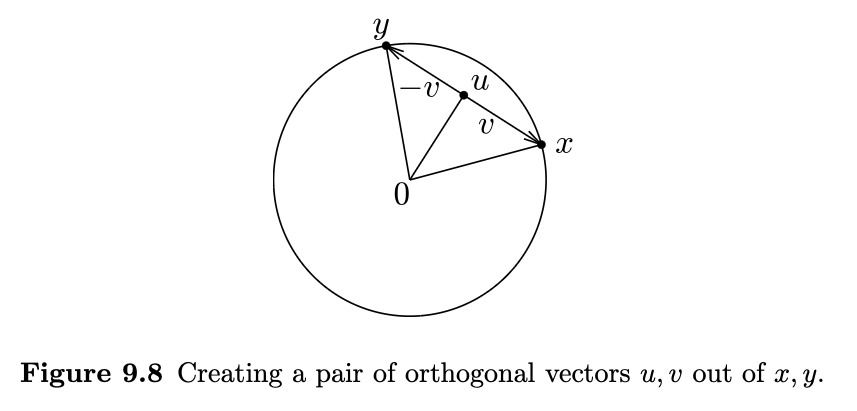
\includegraphics[width=0.8\textwidth]{Chapter 9/fig9-8.png}
\end{center}
Since $u, v$ are orthogonal, the Gaussian random vectors $Au$ and $Av$ are independent (Exercise 3.20).

\textbf{Step 2: Using Gaussian concentration.} Let's condition on $a := Au$ and study the conditional 
distribution of 
\[ f(Ax) = f(a + Av). \]
By independence, $a + Av$ is a Gaussian random vector that we can write as 
\[ a + Av = a + \lVert v \rVert_{2}g, \text{ where } g \sim N(0, I_m) \quad (\text{Exercise 3.20}) \]
We claim that the function 
\[ z \mapsto f(a + \lVert v \rVert_{2}z) \]
is Lipschitz with respect to the Euclidean norm on $\mathbb{R}^m$, with Lipschitz norm bounded by $\lVert v
\rVert_{2}$. To check this, fix any $t, s \in \mathbb{R}^m$ and use subadditivity of $f$ (in the form of 
Exercise 9.34) to get 
\begin{align*}
	f(a + \lVert v \rVert_{2}t) - f(a + \lVert v \rVert_{2}s) 
	&\leq f(\lVert v \rVert_{2}t - \lVert v \rVert_{2}s) \\
	&= \lVert v \rVert_{2} f(t - s) \quad \text{(Positive homogeneity)} \\
	&\leq \lVert v \rVert_{2} \lVert t - s \rVert_{2} \quad (b = 1),
\end{align*}
proving the claim.

Concentration in the Gauss space (\cref{thm:5.2.3}) then yields 
\[ \lVert f(a + Av) - \mathbb{E}_a\left[ f(a + Av) \right] \rVert_{\psi_2(a)}2 \leq C \lVert v \rVert_{2}, \]
where the index ``a" reminds us that these bounds are valid for the conditional distribution with $a = Au$ fixed.

\textbf{Step 3: Removing the conditioning.} Since the random vector $a - Av$ has the same distribution as that 
of $a + Av$, it satisfies the same bound:
\[ \lVert f(a - Av) - \mathbb{E}_a\left[ f(a - Av) \right] \rVert_{\psi_2(a)} \leq C \lVert v \rVert_{2}, \]
Subtract the bottom equation from the top one, use the triangle inequality and the fact that the expectations 
are the same gives 
\[ \lVert f(a + Av) - f(a - Av) \rVert_{\psi_2(a)} \leq 2 C \lVert v \rVert_{2}. \]
This bound holds conditionally for any fixed $a = Au$, Therefore, it holds for the original distribution too:
\[ \lVert f(a + Av) - f(a - Av) \rVert_{\psi_2} \leq 2 C \lVert v \rVert_{2}. \]
Passing back the the $x, y$ notation, we obtained the desired inequality.

We proved the theorem for unit vectors $x, y$. To extend it to the general case, argue exactly as step 4 in the 
proof of \cref{thm:9.1.2}.
\end{proof}

\begin{remark}[]
\label{rmk:9.6.5}
It is an open question if \cref{thm:9.6.3} holds for general subgaussian matrices $A$.
\end{remark}



% ----------9.7----------
\subsection{Two-sided Chevet Inequality and Dvoretzky-Milman Theorem}


\subsubsection{Two-sided Chevet's Inequality}
Another consequence of general matrix deviation is a sharper version of Chevet's inequality:

\begin{theorem}[Two-sided Chevet's inequality]
\label{thm:9.7.1}
Let $A$ be an $m \times n$ Gaussian random matrix with i.i.d $N(0, 1)$ entries. Let $T \subset \mathbb{R}^n$ and 
$S \subset \mathbb{R}^m$ be arbitrary bounded sets. Then 
\[ \mathbb{E}\left[ \sup_{x \in T} \left| \sup_{y \in S}\left\langle Ax, y \right\rangle - w(S) \lVert x 
\rVert_{2} \right| \right] \leq C \gamma(T) \mathrm{rad}(S), \]
where $\gamma(T)$ is the Gaussian complexity and $\mathrm{rad}(T)$ is the radius.
\end{theorem}

\begin{proof}
Let's apply \cref{thm:9.6.3} for the support function of $S$:
\[ f(x) = \sup_{y \in S}\left\langle x, y \right\rangle. \]
This is a bounded function, since the Cauchy-Schwartz inequality gives 
\[ f(x) \leq \sup_{y \in S}\lVert x \rVert_{2}\lVert y \rVert_{2} = \mathrm{rad}(S) \lVert x \rVert_{2} 
\text{ for all } x \in \mathbb{R}^n. \quad (*) \]
Since $Ax$ has the same distribution as $g \lVert x \rVert_{2}$ where $g \sim N(0, I_m)$ from Exercise 3.20, 
we have that 
\begin{align*}
	\mathbb{E}\left[ f(Ax) \right] 
	&= \lVert x \rVert_{2} \mathbb{E}\left[ f(g) \right] \quad (\text{Positive homogeneity}) \\
	&= \lVert x \rVert_{2} \mathbb{E}\left[ \sup_{y \in S}\left\langle x, y \right\rangle \right] \quad 
	\text{(By definition of )} f \\
	&= \lVert x \rVert_{2} w(S) \quad \text{(By definition of Gaussian width)}. \quad (**)
\end{align*}
Substitute $(*)$ and $(**)$ into \cref{thm:9.6.3} completes the proof.
\end{proof}


\subsubsection{Dvoretzky-Milman Theorem}
We'll now prove this amazing result: If you project any bounded set in $\mathbb{R}^n$ to a low-dimensional 
subspace, it will look \textit{approximately round} with high probability (Figure 9.9).

\begin{center}
	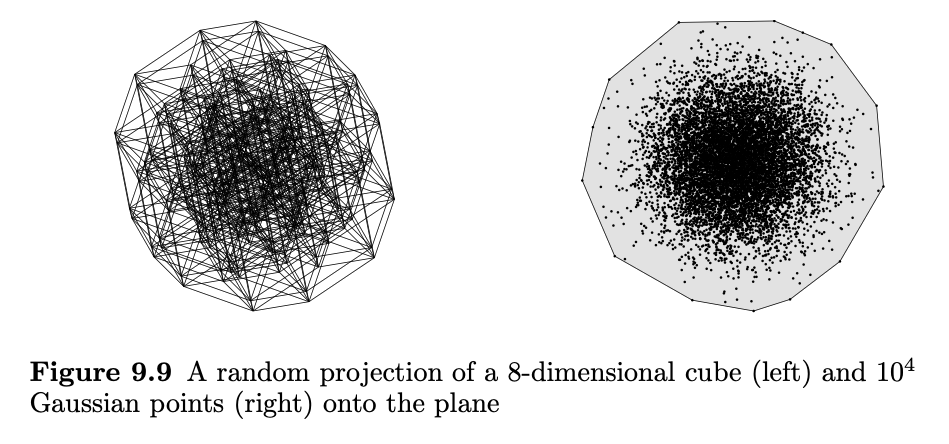
\includegraphics[width=0.8\textwidth]{Chapter 9/fig9-9.png}
\end{center}

It's easier to work with Gaussian projections, where the result says:
\begin{theorem}[Dvoretzky-Milman theorem]
\label{thm:9.7.2}
Let $A$ be an $m \times n$ Gaussian random matrix with i.i.d. $N(0, 1)$ entries, and $T \subset \mathbb{R}^n$ be 
a bounded subset. Then the following holds with probability at least 0.99:
\[ r_- B_2^m \subset \mathrm{conv}(AT) \subset r_+ B_2^m \]
where $B_2^m$ denotes the unit Euclidean ball in $\mathbb{R}^m$, and 
\[ r_{\pm} = w(T) \pm C \sqrt{m} \mathrm{rad}(T). \]
The left inclusion holds only if $r_-$ is nonnegative; the right inclusion always holds.
\end{theorem}

\begin{proof}
Let's use the two-sided Chevet's inequality (\cref{thm:9.7.1}) in the following form:
\[ \mathbb{E}\left[ \sup_{y \in S} \left| \sup_{x \in T}\left\langle Ax, y \right\rangle - w(T) \lVert y 
\rVert_{2} \right| \right] \leq C \gamma(S) \mathrm{rad}(T), \]
where $T \subset \mathbb{R}^n$ and $S \subset \mathbb{R}^m$. To get this, just apply the theorem to $A^T$ with 
$T$ and $S$ swapped.

Let $S$ be the sphere $S^{m - 1}$; its Gaussian complexity satisfies $\gamma(T) \leq \sqrt{m}$. Then, by 
Markov's inequality, the following holds with probability at least 0.99:
\[ \left| \sup_{x \in T}\left\langle Ax, y \right\rangle - w(T) \right| \leq C \sqrt{m} \mathrm{rad}(T) 
\text{ for every } y \in S^{m -1}. \]
By the triangle inequality and the definition of $r_{\pm}$, this implies 
\[ r_- \leq \sup_{x \in T}\left\langle Ax, y \right\rangle \leq r_+ \text{ for every } y \in S^{m - 1}. \]
Rewriting $\sup_{x \in T}\left\langle Ax, y \right\rangle$ as $\sup_{x \in AT}\left\langle x, y \right\rangle$ 
and using homogeneity, we get 
\[ r_- \lVert y \rVert_{2} \leq \sup_{x \in AT}\left\langle x, y \right\rangle \leq r_+ \text{ for every } 
y \in \mathbb{R}^m. \]
By duality (Exercise 9.40), this is the same as the statement of the theorem, and we're done!
\end{proof}

\begin{remark}[The effective dimension]
\label{rmk:9.7.3}
Assume that $T$ is bounded, convex, and contains the origin, and let 
\[ m \leq c d(T) \]
where $d(T) \asymp w(T)^2 / \mathrm{rad}(T)^2$ is the effective dimension (\cref{def:7.5.12}). If we pick the 
absolute constant $c$ to be small enough, we can make $C \sqrt{m} \mathrm{rad}(T) \leq 0.01 w(T)$, so that 
the Dvoretzky-Milman theorem (\cref{thm:9.7.2}) gives
\[ 0.99B \subset AT \subset 1.01B \]
with $B = w(T) B_2^n$ is the Euclidean ball of radius $w(T)$. In short: projecting \textit{any} bounded convex 
set $T$ onto a random subspace of dimension about $d(T)$ makes it look almost like a round ball!
\end{remark}

\begin{example}[Almost round projections of the cube]
\label{ex:9.7.4}
Consider the cube $T = [-1, 1]^n$. By \cref{ex:7.5.7}, 
\[ w(T) = \sqrt{2/\pi} \cdot n \text{ and } \mathrm{diam}(T) = 2 \sqrt{n} \]
So the effective dimension is $d(T) \asymp n$. So, if $m \leq cn$, then with high probability we have 
\[ 0.99B \subset A[-1, 1]^n \subset 1.01B \]
where $B$ is the Euclidean ball with radius $\sqrt{2/\pi} \cdot n$. In short: projecting an $n$-dimensional cube 
onto a subspace of dimension $m = cn$ makes it look almost like a round ball! Figure 9.9 gives an illustration.
\end{example}

\begin{remark}[Summary of random projections]
\label{rmk:9.7.5}
In sections 7.6 and 9.2.2, we found that a random projection $P$ of a set $T$ onto an $m$-dimensional subspace 
in $\mathbb{R}^n$ undergoes a phase transition. In the high-dimensional regime $(m \gtrsim d(T))$, the 
projection shrinks the diameter of $T$ by the factor of order $\sqrt{m/n}$: 
\[ \mathrm{diam}(PT) \asymp \sqrt{\frac{m}{n}} \mathrm{diam}(T)  \]
Moreover, the additive Johnson-Lindenstrauss lemma shows that in this regime, the random projection $P$ 
approximately preserves the geometry of $T$ (the distances between all points in $T$ shrink roughly by the same 
scaling factor).

In the low-dimensional regime $(m \lesssim d(T))$, shrinking stops:
\[ \mathrm{diam}(PT) \asymp w_s(T) \asymp \frac{w(T)}{\sqrt{n}} \]
regardless of how small $m$ is. The Dvoretzky-Milman theorem explains why: $PT$ is now an \textit{approximate 
round ball} of radius of order $w_s(T)$ (Exercise 9.43), which obviously does not shrink under any projection!
\end{remark}




\end{document}

